\documentclass[a4paper,twoside,11pt]{article}
\usepackage{graphicx}
\usepackage{txfonts}
\usepackage{color}
\usepackage{acronym}
\usepackage{textcomp}
\usepackage{url}
\usepackage{upquote} % verbatim apostrophes display as '
\usepackage[hidelinks,hyperfootnotes=false]{hyperref}
\NeedsTeXFormat{LaTeX2e}
\setcounter{tocdepth}{5}
\setcounter{secnumdepth}{5}
%% Include layout, additional commands and abbreviations
%%
%% Layout definitions
%%

\usepackage[english]{babel}
\usepackage{lastpage}
\usepackage{multirow}
\usepackage{longtable}
\usepackage{supertabular}
\usepackage{fancyhdr}
\usepackage{graphicx}
\usepackage{makeidx}
\usepackage[figuresright]{rotating}

\usepackage{times}
\usepackage{verbatim}
\usepackage{dmd-doc}

\renewcommand{\encodingdefault}{T1}

\makeatletter
\renewcommand\paragraph{\@startsection{paragraph}{4}{\z@}%
  {-3.25ex\@plus -1ex \@minus -.2ex}%
  {0.2ex \@plus 0.2ex}%
  {\normalfont\normalsize\bfseries}}
\makeatother

%%% Local Variables: 
%%% mode: latex
%%% TeX-master: t
%%% End: 


%% $Id: shortcut.tex,v 1.3 2003/12/12 09:13:51 cizzo Exp $
%% Abbreviations and extra command definitions
%%

%%
%% Additional commands
%%
\newcommand{\cm}[1]{\marginpar{\scriptsize #1}}

\newcommand{\tbspa}{\rule[1ex]{0pt}{1.1ex}}
\newcommand{\tbspb}{\rule[-1.0ex]{0pt}{1.0ex}}


%%
%% Abbreviations
%%

\newcommand{\eg}{{\it e.g.}}
\newcommand{\ie}{{\it i.e.}}

\newcommand{\degr}{\hbox{$^\circ$}}
\newcommand{\arcmin}{\hbox{$^\prime$}}
\newcommand{\arcsec}{\hbox{$^{\prime\prime}$}}

\newcommand{\CPL}{\textit{Common Pipeline Library}}
\newcommand{\mf}{{\tt molecfit}}

% Added to standard shortcuts:
\newcommand{\radunits}
{${\rm phot\,s}^{-1}\,{\rm m}^{-2}\,$\textmu${\rm m}^{-1}\,{\rm arcsec}^{-2}$}

\newcommand{\mum}{\textmu m}

%%% Local Variables: 
%%% mode: latex
%%% TeX-master: t
%%% End: 


\dmdTitle{SKYCORR sky correction: \\[0.2cm] User documentation and evaluation}
\dmdDocId{VLT--MAN--ESO--19550--5896}
\dmdIssue{4.4}
\dmdDate{2014--04--01}

\dmdPreparedBy{Innsbruck ESO In-Kind Team}
\dmdPreparedOn{2014--04--01}
\dmdApprovedBy{***TBD***}
\dmdApprovedOn{}
\dmdReleasedBy{***TBD***}
\dmdReleasedOn{}

\setlongtables
\makeindex                              % but currently no indexed terms...

\begin{document}
\pagenumbering{arabic}
\dmdmaketitle
\emptypage{This page was intentionally left blank}

\begin{center}
  \textbf{Change record}

  \tablehead{\hline
    \multicolumn{1}{|c|}{Issue/Rev.}\tbspa &
    \multicolumn{1}{|c|}{Date} &
    \multicolumn{1}{|c|}{Section/Parag.\ affected} &
    \multicolumn{1}{|c|}{Reason/Initiation/Documents/Remarks}\tbspb \\
    \hline}
  \tabletail{\hline}

  \begin{supertabular}{|l|l|l|l|}
    4.4\tbspa & 01/04/2014 & Sect. 3                                    &
              Update installation instructions                          \\
    4.3\tbspa & 20/09/2013 & All                                        &
              RIXes for final review considered                         \\
    4.2\tbspa & 30/07/2013 & All                                        &
              Changes related to code-testing workshop                  \\
    & & &     Sky model update                                          \\
    4.1\tbspa & 13/05/2013 & Sect. 4 and 5.2                            &
              Parameter description, routine extract1D, examples        \\
    4.0\tbspa & 30/04/2013 & All                                        &
              Focus on C code, extended I/O options                     \\
    3.4\tbspa & 03/05/2012 & Sect. 4.2 and 5                            &
              Description of conversion of FITS 1D images               \\
    & & &     Update of the Reflex workflow description                 \\
    3.3\tbspa & 16/03/2012 & Sect. 3, 4, 6                              &
              Some rephrasing, Figs. 24-29 changed                      \\
    3.2\tbspa & 09/03/2012 & Sect. 3.2, 4.6, 4.7                        &
              Updating installation and running procedure               \\
    3.1\tbspa & 18/11/2011 & Sect. 6.4 and 7                            &
              Update related to line list change                        \\
    3.0\tbspa & 08/09/2011 & All                                        &
              General update                                            \\
    2.0\tbspa & 31/07/2011 & All                                        &
              General update                                            \\
    1.0\tbspa & 01/06/2011 & All                                        &
              First version                                             \\
  \end{supertabular}
\end{center}

%Temporary list concerning already considered RIXes:
%JLI: 20, 21, 22, [23], [24], 25
%AMO: 1, 2, 3
%?: needs check, (): partly done, []: no change required

\begin{center}
\textbf{Main authors (Austrian ESO In-Kind Team Innsbruck)}
  \tablehead{
    \hline}
  \tabletail{\hline}

  \begin{supertabular}{|c|}
    \\
    Wolfgang Kausch \\
    Stefan Noll \\
    Marco Barden \\
    Cezary Szyszka \\
    Amy M. Jones \\
    Stefan Kimeswenger \\
    \\
    Institute for Astro- and Particle Physics,
    University of Innsbruck \\
    Technikerstr. 25/8 \\
    A-6020 Innsbruck / Austria \\
    \\
  \end{supertabular}
\end{center}

\emptypage{This page was intentionally left blank}

\tableofcontents
\cleardoublepage
%-------------------------------------------------------------------------------
\section{Introduction}\label{sec:introduction}
%-------------------------------------------------------------------------------
This document is intended to be a user documentation/manual of the sky
correction code SKYCORR developed within the framework of the Austrian
\acs{ESO} In-Kind SM project as described in the corresponding Statement of
Work document \cite{SM-SoW}.

The aim of the SKYCORR project is to provide an advanced instrument-independent
sky-correction tool that removes sky emission in science spectra by means of
sky spectra taken at a different time and sky location. The algorithm adapts a
reference sky spectrum to a science spectrum by correcting differences due to
temporal and spatial airglow variability and issues related with the instrument
or the data reduction\footnote{For multi-object and integral-field
spectroscopy, it could be prudent to correct with a reference sky spectrum
taken from the same exposure. In this case, SKYCORR would mainly be used to
correct for instrumental effects.}. The approach is based on a similar method
for SINFONI near-IR spectroscopic data described in Davies \cite{DAV07}.

This document is organised as follows: Section~\ref{sec:overview} gives a
brief overview on the project and the incorporated algorithms.
Section~\ref{sec:installation} provides information on the installation
procedure. Section~\ref{sec:running} contains a description of how to run the
code, the required input parameter file, and the output files.
Section~\ref{sec:method} explains the adapted sky correction method and the
airglow model in detail. Finally, the code performance is evaluated in
Section~\ref{sec:evaluation} by means of a test data set.

%-------------------------------------------------------------------------------
\section{Overview}\label{sec:overview}
%-------------------------------------------------------------------------------
%-------------------------------------------------------------------------------
\subsection{The Davies method}\label{sec:davies}
%-------------------------------------------------------------------------------
For spectroscopic instrument set-ups and observing programmes that do not
provide pure sky spectra in parallel to the desired object spectra (\eg\
two-dimensional long-slit spectra where the object does not cover the whole
slit), it is necessary to use sky spectra taken at a different time as the
science spectra for the sky correction. However, the strong variability of
airglow emission on time scales in the order of a few minutes can
cause unavoidable sky correction residua. Significant changes in the airglow
emission can also be expected for sky position differences in the order of a
few degrees or even less depending on the characteristics of possible wave
patterns. Moreover, different telescope positions and ambient conditions may
cause instrument flexures, which result in shifting of the sky with regard to
the science spectrum. Hence, the reference sky spectrum has to be adapted in
both, the flux and the wavelength regime, to allow a reasonable sky background
correction.

An illustration of this problem and a solution for SINFONI has been described
by Davies \cite{DAV07}. The airglow correction method proposed in this paper is
based on applying arbitrary sky spectra to science spectra by scaling
physically related OH line groups of the sky spectrum to the corresponding
groups in the science spectrum. Subsequently, the newly created scaled spectrum
is used for the sky correction. Specifically, the Davies method groups emission
lines from vibrational-rotational transitions resulting from non-thermal
excitation processes of the OH molecule and defines wavelength regions where
these groups dominate the airglow emission. These wavelength ranges are scaled
in the sky spectrum to match the corresponding flux in the object spectrum.
This approach only works for the line component of the sky emission. Since
object and sky continua cannot satisfyingly be separated, the sky continuum
cannot be adapted and has to be subtracted before the scaling procedure for the
line emission can start. Since the Davies method is restricted to OH airglow
lines beyond 1\,$\mu$m\footnote{The version 2.0 of Davies' code also allows
simple scaling of the strong O$_2$ band at 1.27\,$\mu$m. This feature is not
described in Davies \cite{DAV07}.}, it can only be applied in near-IR
wavelength regions where other line emission is negligible. This method has
been implemented for SINFONI (Modigliani et al. \cite{MOD07}).

%-------------------------------------------------------------------------------
\subsection{Improvements of the Davies method}
\label{sec:improvements}
%-------------------------------------------------------------------------------
In the framework of the SM subproject ``Advanced sky model'', an extended
semi-empirical model for airglow emission was developed (see \cite{SM01} User
Manual and Noll et al. \cite{NOL12}). It is based on the OH line list by
Rousselot et al. \cite{ROU00}. Also, it incorporates the empirical
--mainly optical-- line list by Hanuschik \cite{HAN03} and Cosby et al.
\cite{COS06} based on high-resolution UVES observations, and the HITRAN
database for molecular data \cite{HITRAN}. Additionally, five variability
classes were introduced for the entire line list (\ie\ green O\,I, Na\,D, red
O\,I, OH, and O$_2$, see Section~\ref{sec:airglow}) in order to take into
account intensity variations due to changes of the solar activity, the season,
and the time during the night. The variability correction recipes for the
different classes were calculated from 1189 VLT FORS sky spectra (Patat
\cite{PAT08}).

For SKYCORR, this model is extended by identifications of lines with similar
upper and lower electronic, vibrational, and/or rotational states that are
expected to vary in a very similar way (more similar than the lines belonging
to the relatively rough variability classes defined in Noll et al.
\cite{NOL12}). If the spectral resolution is given, the airglow emission
model with the improved line list (ranging from 0.3 to 2.5\,$\mu$m) allows
deriving the contributions of different line groups to the pixels of a sky
spectrum. Hence, in wavelength space overlapping groups can be handled by such
an implementation contrary to the Davies method, which uses fixed wavelength
intervals. The optimum scaling of the different line groups is then derived by
means of a fitting procedure that is not required for the simpler approach of
Davies. This fitting procedure also allows the wavelength grid to be adapted.
Similar to \cite{MOLECFIT}, the adaptation process is based on Chebyshev
polynomials and subpixel shifts instead of simple shifting by full pixels only.
In general, the new method should be applicable to all wavelength regions where
airglow emission plays an important role. Hence, apart from SINFONI, the
SKYCORR code is also appropriate for correcting spectroscopic observational
data from, \eg, ISAAC, X-Shooter, VIMOS, or FORS.

%-------------------------------------------------------------------------------
\subsection{Algorithm}\label{sec:algorithm}
%-------------------------------------------------------------------------------
The algorithm used by the SKYCORR code is sketched in
Figure~\ref{fig:skycorr_overview}. Its main purpose is the removal of sky
emission lines in a science spectrum by means of a scaled reference sky
spectrum. To this end, any continuum flux in the input science and reference
sky spectra has to be removed in advance. Hence, as a first step, pixels
belonging to lines and continuum have to be identified, separated, and masked
accordingly. The second step is a fit to continuum pixels only, which is
subtracted from the input spectrum to obtain a continuum-free spectrum. In the
third step, a weight mask for the different airglow line groups in the
reference sky spectrum is calculated incorporating the extended sky model
mentioned above. The actual line and wavelength fitting process is performed in
step four (incorporating the MPFIT library \cite{CMPFIT}). Here, the reference
sky line spectrum is fitted to the emission lines in the science spectrum.
Finally, the best-fit sky line spectrum and the uncorrected sky continuum
spectrum are subtracted from the input science spectrum. More details on this
approach can be found in Section~\ref{sec:method}.

%-------------------------------------------------------------------------------
\begin{figure}[ht]
  \begin{center}
    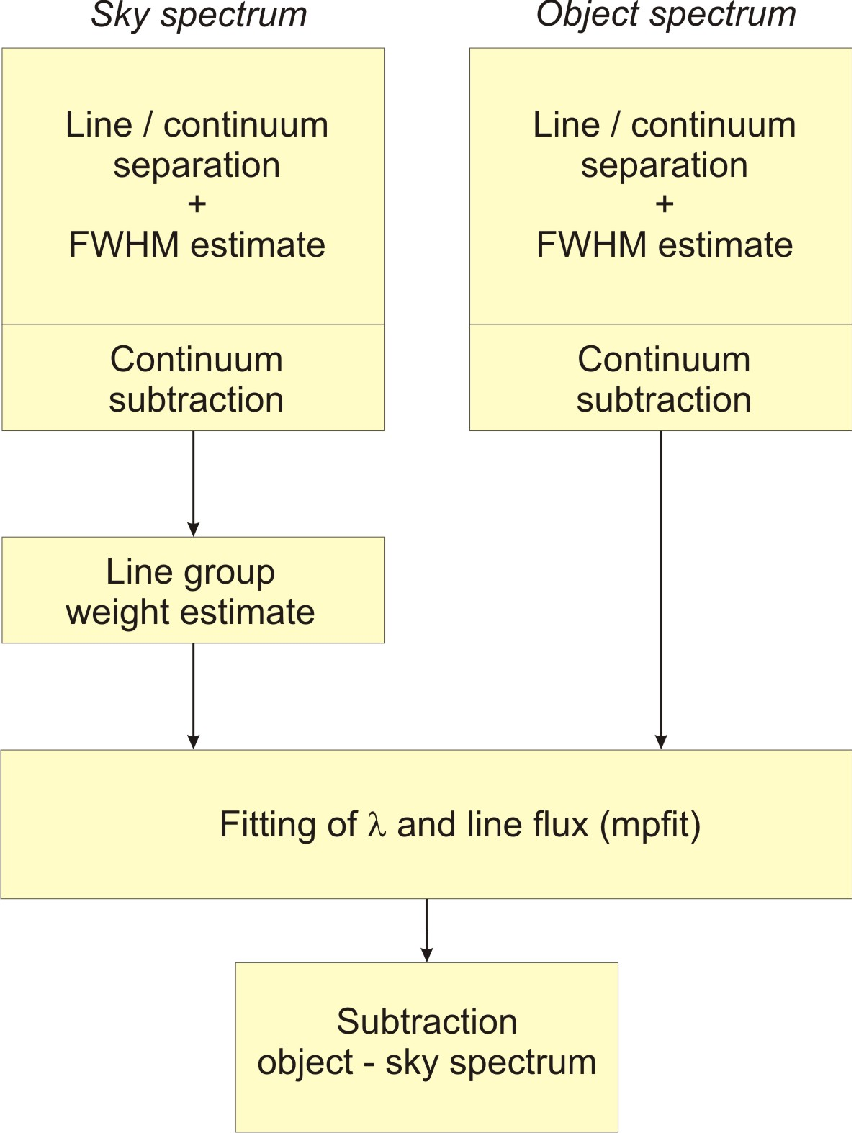
\includegraphics[width=0.9\textwidth]{figures/skycorr_workflow_scheme.png}
    \caption{{\it Overview of the SKYCORR project workflow}.}
    \label{fig:skycorr_overview}
  \end{center}
\end{figure}
%-------------------------------------------------------------------------------

\cleardoublepage
%-------------------------------------------------------------------------------
\section{Installation procedure}\label{sec:installation}
%-------------------------------------------------------------------------------
%-------------------------------------------------------------------------------
\subsection{Requirements}\label{sec:requirements}
%-------------------------------------------------------------------------------
The installation of the basic SKYCORR binary package requires:
\begin{itemize}
  \item
    C99 compatible compiler (e.g. gcc or clang)
  \item
    glibc 2.11 or newer on Linux or OS X 10.7 or newer
  \item
    common unix utilities (bash, tar, sed, grep, \ldots{})
\end{itemize}

The optional \ac{GUI} to SKYCORR requires:

\begin{itemize}
  \item
    Python v2.6 or v2.7 (but not Python v3.x)
  \item
    wxPython v2.8 or newer
  \item
    Python matplotlib v1.0 or newer
  \item
    PyFITS v2.4 or newer
\end{itemize}

The command line client also has optional display features which
require:

\begin{itemize}
  \item gnuplot v4.2 patchlevel 3 or newer
\end{itemize}

%-------------------------------------------------------------------------------
\subsection{Binary installation}
\label{sec:installscript}
%-------------------------------------------------------------------------------

First the downloaded installer needs to be made executable. To do this change
into the directory the installer was downloaded to and run following command
(replacing {\tt skycorr\_installer.run} with the actual downloaded filename):

\begin{verbatim}
chmod u+x ./skycorr_installer.run
\end{verbatim}

Now the installer can be executed from the same folder with:

\begin{verbatim}
./skycorr_installer.run
\end{verbatim}

It will ask for an installation directory where it will extract its
contents to. It is recommended to choose an empty directory to avoid
overwriting existing files.

After the installer has successfully finished, the {\tt skycorr} executables
are installed into the \texttt{bin} subdirectory of the chosen installation
folder. They can be executed by specifying the full or relative path.
Also installed are a set of example parameter files for several
instruments in the \texttt{examples/config} directory. To run a SINFONI example
type:

\begin{verbatim}
<INST_DIR>/bin/skycorr <INST_DIR>/examples/config/sctest_sinfo_H.par
\end{verbatim}

For more details see Section~\ref{sec:running}.

The following directory structure is created by the installation routine:

\begin{verbatim}
   <INST_DIR>
        |
        |-- bin
        |-- config
        |-- doc
        |-- examples
        |       |-- config
        |       |-- data
        |       |-- sysdata -> <INST_DIR>/sysdata/
        |-- output
        |-- sysdata

\end{verbatim}
In detail:
\begin{itemize}
  \item {\tt bin/}: location of binary files
  \item {\tt config/}: directory containing template configuration files
  \item {\tt doc/}: documentation
  \item {\tt examples/}: directory with examples
  \item {\tt output/}: default output directory
  \item {\tt sysdata/}: directory containing data required for SKYCORR
\end{itemize}


%-------------------------------------------------------------------------------
\subsection{\ac{GUI} dependencies}
\label{sec:guidependencies}
%-------------------------------------------------------------------------------

The \ac{GUI} requires some additional dependencies to be installed on the system. To
check if the python installation is able to run the \ac{GUI}, following
commands can be run:

\begin{verbatim}
python -c 'import wx'

python -c 'import matplotlib; import matplotlib.backends.backend_wxagg'

python -c 'import pyfits'
\end{verbatim}

If these commands fail please see following site for instructions on how
to install these packages:

\texttt{http://www.eso.org/pipelines/reflex\_workflows/}

%-------------------------------------------------------------------------------
\subsection{Package contents}
\label{sec:pkgcontents}
%-------------------------------------------------------------------------------

The installation package is a self extracting tarball containing the
SKYCORR source code and pre-built versions of its third party dependencies:

\begin{itemize}
  \item
    Common Pipeline Library v6.4.2 and its dependencies cfitsio v3.350,
    wcslib v4.16 and fftw3 v3.3.3 \cite{CPL}
\end{itemize}


%-------------------------------------------------------------------------------
\subsection{Source Installation}
\label{sec:sourceinstall}
%-------------------------------------------------------------------------------

Advanced users may want to install everything from source, the
basic instructions for this are outlined in this section.

\subsubsection{CPL compilation}

The CPL sources can be obtained from \cite{CPL}

CPL only requires cfitsio in order to run SKYCORR. It can be installed as
follows:

\begin{verbatim}
./configure --prefix=/install-location

make

make shared

make install
\end{verbatim}

Then CPL can be install with:

\begin{verbatim}
./configure --prefix=/install-location --with-cfitsio=/install-location

make

make install
\end{verbatim}

See the respective packages documentation for details on the
installation procedure.

\subsubsection{SKYCORR compilation}

After all dependencies have been installed SKYCORR can be compiled from source
into the same location.

This is the only step required if one wants to update SKYCORR from
source after previously installing the third party dependencies with the
binary installer.

\begin{verbatim}
./configure --prefix=/install-location --with-cpl=/install-location

make

make install
\end{verbatim}

In order to use SKYCORR from this location the environment variable
{\tt LD\_LIBRARY\_PATH} \\(or {\tt DYLD\_LIBRARY\_PATH} on Mac OS) need to be
set. With the bash shell this is done with following command:

\begin{verbatim}
export LD_LIBRARY_PATH=/install-location/lib
\end{verbatim}

Now {\tt skycorr} is ready to be used from {\tt /install-location/bin}.

\cleardoublepage
%-------------------------------------------------------------------------------
\section{Code execution procedure}\label{sec:running}
%-------------------------------------------------------------------------------
This section describes how to use the SKYCORR software.
Section~\ref{sec:paramfile} provides an example for an input parameter file.
The input parameters are discussed in detail in Section~\ref{sec:params}.
Finally, the output of the code is described in Section~\ref{sec:output}. In
Section~\ref{sec:calling} the execution of the programme is shown. For the
extraction of 1D spectra suitable for SKYCORR from 2D FITS images, see
Section~\ref{sec:extract1d}. The run of examples is described in
Section~\ref{sec:calling_examples}. The SKYCORR software also provides a Reflex
workflow. It is discussed in Section~\ref{sec:reflex}.

%-------------------------------------------------------------------------------
\subsection{Input parameter file}\label{sec:paramfile}
%-------------------------------------------------------------------------------
All parameters needed for the fit are read from an ASCII parameter file, which
contains parameter names, descriptions, and initial values. In the following,
{\tt src/test/config/sctest\_sinfo\_H.par} is shown as an example of a
parameter file. Individual parameters are explained in
Section~\ref{sec:params}:

{\small
\begin{verbatim}
# ----------------------------------------------------------------------------
# -------------------- INPUT PARAMETER FILE FOR SKYCORR ----------------------
# ----------------------------------------------------------------------------

# ---------------------------DIRECTORIES + FILES------------------------------

# Absolute path of skycorr installation directory
INST_DIR=../../

# Absolute or relative (with respect to INST_DIR) path and filename of input
# object spectrum
INPUT_OBJECT_SPECTRUM=src/test/data/sky_sinfo_1.fits

# Absolute or relative (with respect to INST_DIR) path and filename of input
# sky spectrum
INPUT_SKY_SPECTRUM=src/test/data/sky_sinfo_2.fits

# Absolute or relative (with respect to INST_DIR) path and filename of output
# directory (will be created if not present; default: <INST_DIR>/output/)
OUTPUT_DIR=output

# Main name of diagnostic output files, extensions will be added
OUTPUT_NAME=TEST-SINFO-H

#------------------------------INPUT STRUCTURE--------------------------------

# Names of file columns (table) or extensions (image)
# A list of 4 labels has to be provided:
# 1: wavelength [image: NONE if dedicated extension does not exist]
# 2: flux [image: NONE if in zeroth, unnamed extension]
# 3: flux error [NONE if not present]
# 4: mask (integer: 1 = selected, 0 = rejected;
#          float:   0. = selected, otherwise rejected) [NONE if not present]
COL_NAMES=lambda flux NONE NONE

# Error relative to mean if no error column is provided (default: 0.01)
DEFAULT_ERROR=0.01

# Multiplicative factor to convert wavelength to micron
# e.g.: wavelength unit = A -> WLG_TO_MICRON = 1e-4
WLG_TO_MICRON=1.

# Wavelengths in vacuum (= vac) or air (= air)
VAC_AIR=vac


# ----------------------------------------------------------------------------
# ------------------------- EXPERT MODE PARAMETERS ---------------------------
# ----------------------------------------------------------------------------

# ------------------------------FITS KEYWORDS---------------------------------

# FITS keyword of sky spectrum for Modified Julian Day (MJD) or date in years
# (default: MJD-OBS; optional parameter for value: DATE_VAL)
DATE_KEY=MJD-OBS

# FITS keyword of sky spectrum for UTC time in s
# (default: TM-START; optional parameter for value: TIME_VAL)
TIME_KEY=TM-START

# FITS keyword of sky spectrum for telescope altitude angle in deg
# (default: ESO TEL ALT; optional parameter for value: TELALT_VAL)
TELALT_KEY=ESO TEL ALT

# ---------------------------REQUIRED INPUT DATA------------------------------

# Airglow line list
# Required directory: <INST_DIR>/sysdata/
LINETABNAME=airglow_groups.dat

# File for airglow scaling parameters
# Required directory: <INST_DIR>/sysdata/
VARDATNAME=airglow_var.dat

# FTP address (supplemented by "ftp://") for folder with monthly averages of
# solar radio flux at 10.7 cm
SOLDATURL=ftp.geolab.nrcan.gc.ca/data/solar_flux/monthly_averages

# File with monthly averages of solar radio flux at 10.7 cm
# Required directory: SOLDATURL or <INST_DIR>/sysdata/
SOLDATNAME=solflux_monthly_average.txt

# Solar radio flux at 10.7 cm:
# Positive value in sfu (= 0.01 MJy) or -1 [default] for corresponding monthly
# average from http://www.spaceweather.gc.ca. Download only if local file in
# <INST_DIR>/sysdata/ does not contain required month.
SOLFLUX=-1

# ---------------------------LINE IDENTIFICATION------------------------------

# Initial estimate of line FWHM [pixel]
FWHM=5.0

# Variable line width (linear increase with wavelength)? -- 1 = yes; 0 = no
VARFWHM=0

# Relative FWHM convergence criterion (default: 1e-2)
LTOL=1e-2

# Minimum distance to neighbouring lines for classification as isolated line:
# <MIN_LINE_DIST> * <FWHM> [pixel]
MIN_LINE_DIST=2.5

# Minimum line peak flux for consideration of lines from airglow line list:
# <FLUXLIM> * <median flux of identified lines>
# Automatic search -> FLUXLIM = -1 (default)
FLUXLIM=-1

# ---------------------------FITTING OF SKY LINES-----------------------------

# Relative chi^2 MPFIT convergence criterion (default: 1e-3)
FTOL=1e-3

# Relative parameter MPFIT convergence criterion (default: 1e-3)
XTOL=1e-3

# Relative chi^2 convergence criterion for iterative improvement of
# wavelength grid (default: 1e-3)
WTOL=1e-3

# Maximum degree of Chebyshev polynomial for wavelength grid correction:
# -1 = no correction
#  0 = linear term (coef. = 1) is also considered but not fitted
#  7 = default
CHEBY_MAX=7

# Minimum degree of Chebyshev polynomial for wavelength grid correction.
# CHEBY_MIN <= CHEBY_MAX:
# - Iterative increase of polynomial degree at least until CHEBY_MIN
#   (default: 3).
# - Procedure stops if chi^2 gets worse or CHEBY_MAX is reached.
# - Results of degree with best chi^2 are taken.
# CHEBY_MIN > CHEBY_MAX:
# - Iterative increase of polynomial degree until CHEBY_MAX is reached.
# - Results of degree CHEBY_MAX are taken.
CHEBY_MIN=3

# Initial constant term for wavelength grid correction (shift relative to half
# wavelength range)
CHEBY_CONST=0.

# Type of rebinning:
# 0 = simple rebinning (summation of pixel fractions)
# 1 = convolution with asymmetric, damped sinc kernel [default]
REBINTYPE=1

# Minimum relative weight of the strongest line group of a pixel for
# including a pixel in the line fitting procedure (default: 0.67)
WEIGHTLIM=0.67

# Sigma limit for excluding outliers (e.g. object emission lines) from
# estimate of group flux correction factors (default: 15.)
SIGLIM=15.

# Lower relative uncertainty limit for the consideration of a line group for
# the fitting procedure. The value is compared to the sigma-to-mean ratio of
# the group-specific flux correction factors of the initial estimate
# (default: 0. -> include all fittable line groups).
FITLIM=0.

# ---------------------------------PLOTTING-----------------------------------

# Diagnostic gnuplot plots:
# Options for output on screen:
# W - wxt terminal
# X - x11 terminal
# N - no screen output [default]
# NOTE: An illustration of the sky subtraction quality is plotted into a PS
#       file in the OUTPUT_DIR folder in any case.
PLOT_TYPE=N
\end{verbatim}
}

%-------------------------------------------------------------------------------
\subsection{Parameter description}\label{sec:params}
%-------------------------------------------------------------------------------
In the following, the individual parameters are explained in more detail in the
order as they appear in the parameter file. The file is divided into two parts.
The first part contains the parameters which provide the paths, file names, and
data structures. They have to be adapted if the input and output data files
change. However, the sky correction code can be run without modifying the
parameters of the second part, which affect the sky correction optimisation.
The modification of these so-called expert mode parameters can improve the sky
subtraction provided that the user is willing to run the code several times in
order to find the optimal parameter set.

{\bf\large\tt Basic parameters:}
\begin{itemize}
\item {\sc inst\_dir}: Installation directory for the data reduction task. In
the case of automatic installation (see Section\,\ref{sec:installscript}), this
has to be an absolute path and must be the same as given during the
installation procedure.
\item {\sc input\_object\_spectrum}: Absolute or relative (with respect to
{\sc inst\_dir}) path and name of the input object spectrum for the sky
subtraction procedure. Currently, \ac{ASCII} tables, \ac{FITS} tables with one
table extension, and 1D \ac{FITS} images are allowed. The number of table
columns or \ac{FITS} file image extensions is not restricted. However, only
a single column/extension with flux data can be provided. Corresponding
columns/extensions for flux errors and mask values are also possible. See also
{\sc col\_names}.
\item {\sc input\_sky\_spectrum}: Absolute or relative (with respect to
{\sc inst\_dir}) path and name of the reference input sky spectrum for the sky
subtraction procedure. For the accepted file formats, see
{\sc input\_object\_spectrum}.
\item {\sc output\_dir}: Absolute or relative (with respect to {\sc inst\_dir})
path to the output directory. The folder will be created if it does not exist.
\item {\sc output\_name}: Unique name space for output files. The extensions
{\it \_sci.fits}, {\it \_sky.fits}, {\it \_fit.fits}, {\it \_fit.ps}, and
{\it .res} are added. See Section~\ref{sec:output} for more details.
\item {\sc col\_names}: Column names of the two input files containing
information on wavelength, flux, flux error, and mask. The latter two are
optional and can be disabled by setting them to {\it NONE}. An example
would be the following string: {\it lambda flux NONE NONE}. {\it Blanks} are
used as column name separators. For \ac{ASCII} files, which have to provide the
columns in the given order, the column names are irrelevant, with the exception
of {\it NONE} input. In the case of \ac{FITS} images, the given labels are
compared to the \ac{FITS} extension names (keyword ``EXTNAME''). If there is no
extension name for the spectral flux, it is expected to be present in the first
layer of the \ac{FITS} file (0th extension). In this case, the flux column name
has to be set to {\it NONE}. The name of the wavelength column should also be
{\it NONE}, if the wavelength grid is derived from \ac{FITS} header keywords.
This is the typical situation for \ac{FITS} images. By default, it is expected
that an optional mask has only the values 0 and 1 for rejection and selection,
respectively. Alternatively, pixels with a mask value of 0 are selected
(reverse definition) if the other values (to be rejected) do not equal 1 and
are floating-point numbers.
\item {\sc default\_error}: Default error relative to the mean in the case of
a lacking error column (column name = {\it NONE}, see previous record).
\item {\sc wlg\_to\_micron}: Multiplicative factor to convert input wavelength
unit to micron. For example, for nm this parameter has to set to $10^{-3}$.
\item {\sc vac\_air}: Wavelengths of the input spectra in vacuum ({\it vac}) or
air ({\it air}).
\end{itemize}

{\bf\large\tt Expert mode parameters:}
\begin{itemize}
\item {\sc date\_key}: \ac{FITS} keyword of {\sc input\_sky\_spectrum} for
Modified Julian Day (MJD) or date in years. By default, {\it MJD-OBS} is taken.
If \ac{ASCII} files are provided or no suitable \ac{FITS} keyword is available,
the information has to be provided manually (see below).
\item {\sc date\_val}: MJD or date in years for {\sc input\_sky\_spectrum}.
This parameter is only required if a suitable \ac{FITS} header is not provided
by the input spectrum.
\item {\sc time\_key}: \ac{FITS} keyword of {\sc input\_sky\_spectrum} for UTC
time in seconds. By default, {\it TM-START} is taken. If {\it TM-START} is not
available, an equivalent keyword could be {\it UTC}. If \ac{ASCII} files are
provided or no suitable \ac{FITS} keyword is available, the information has to
be provided manually (see below).
\item {\sc time\_val}: UTC time in seconds for {\sc input\_sky\_spectrum}. This
parameter is only required if a suitable \ac{FITS} header is not provided by
the input spectrum.
\item {\sc telalt\_key}: \ac{FITS} keyword of {\sc input\_sky\_spectrum} for
telescope altitude angle in deg. By default, {\it ESO TEL ALT} is taken. If
\ac{ASCII} files are provided or no suitable \ac{FITS} keyword is available,
the information has to be provided manually (see below).
\item {\sc telalt\_val}: Telescope altitude angle in deg for
{\sc input\_sky\_spectrum}. This parameter is only required if a suitable
\ac{FITS} header is not provided by the input spectrum.
\item {\sc linetabname}: Name of the input airglow line list. The file must be
located in the directory {\tt <inst\_dir>/ sysdata}.
\item {\sc vardatname}: File for the scaling parameters of the airglow
variability model described in Section~\ref{sec:airglow}. The file must be
located in the directory {\tt <inst\_dir>/ sysdata}.
\item {\sc soldaturl}: FTP address (supplemented by {\it ftp://}) for folder
with monthly averages of the solar radio flux at 10.7\,cm. Currently, the link
is provided by {\tt www.spaceweather.gc.ca} and can be obtained via ftp by
\url{ftp.geolab.nrcan.gc.ca/data/solar_flux/monthly_averages}.
\item {\sc soldatname}: Name of file with monthly averages of the solar radio
flux at 10.7\,cm. The file must be located in the directory
{\tt <inst\_dir>/sysdata}. The radio flux is taken from the column
{\it obsflux}. If the data for the required month (as derived from the
\ac{FITS} header) is not present in the local file, the latter is substituted
by the most recent file of the same name in the remote {\sc soldaturl} folder.
In the case of errors a solar radio flux of 130\,sfu is assumed, which
corresponds to the mean of the solar cycles 19 to 23.
\item {\sc solflux}: Solar radio flux at 10.7\,cm in sfu~(= 0.01 MJy). The
default value of -1 results in using the corresponding monthly average from the
file {\sc soldatname}.
\item {\sc fwhm}: Initial guess for the FWHM of the airglow lines in pixels.
This start value is improved by an iterative approach (see
Section~\ref{sec:FWHM}). The width of the sky lines is required for line
identification as well as for the computation of the airglow model.
\item {\sc varfwhm}: Flag for selecting a constant (= 0) or a variable line
width (= 1). In the latter case, all FWHM values are related to the central
wavelength of the full wavelength range. The variable FWHM increases linearly
with wavelength, \ie\ the resolution is constant. X-Shooter Echelle spectra
show this behaviour. For spectra where the object profile in the slit mainly
determines the FWHM, the default constant width option is recommended.
\item {\sc ltol}: Relative FWHM convergence criterion for iterative derivation
of the mean line width in the object and reference sky spectrum (see
Section~\ref{sec:FWHM}). The default is $1 \times 10^{-2}$. In the case of 1,
the code would just use the first FWHM estimate without further iteration.
\item {\sc min\_line\_dist}: Minimum distance to neighbouring lines divided by
the FWHM. This factor is required for the line finding algorithm.
\item {\sc fluxlim}: Minimum line peak flux for including lines from the
airglow line list {\sc linetabname} in the fit. The given value is multiplied
by the median flux of the lines directly identified in the spectrum (see
Section~\ref{sec:linesearch}). The default value of -1 indicates an iterative
approach for the selection of line list entries that aims at including as
many lines as possible without loosing too many pixels for the continuum
interpolation (see Sections~\ref{sec:linesearch} and ~\ref{sec:contsub}). If
the warnings ``no isolated lines found'' and ``all weights =~0'' should appear,
it might help to select a {\sc fluxlim} value below the start value 0.005 of
the automatic search.
\item {\sc ftol}: Relative $\chi^2$ convergence criterion of the MPFIT
least-squares minimisation algorithm for the adaptation of the reference sky
spectrum to the sky in the object spectrum (see Section~\ref{sec:linefit}).
The default is $1 \times 10^{-3}$, \ie, if $\chi^2$ changes between two
iterations by less than 0.1\% the fitting process is stopped.
\item {\sc xtol}: Relative parameter convergence criterion. {\sc xtol} has a
similar functionality as {\sc ftol} but for the fit parameter values instead of
$\chi^2$. The default is $1 \times 10^{-3}$.
\item {\sc wtol}: Relative $\chi^2$ convergence criterion for iterative
adaptation of the wavelength grid of the reference sky spectrum to the grid of
the object spectrum (see Section~\ref{sec:wavegrid}). The degree of the
Chebyshev polynomial that is used to correct the wavelength solution is
increased by 1 for each new iteration. If the resulting $\chi^2$ does not
show a relative improvement of {\sc wtol} and more, the convergence is reached
and the procedure is stopped if {\sc cheby\_min} is not larger than the
polynomial degree of the ongoing iteration (see below). The default is
$1 \times 10^{-3}$.
\item {\sc cheby\_max}: Maximum degree of Chebyshev polynomial for refined
wavelength solution (see Section~\ref{sec:wavegrid}). The special case -1
indicates that no adaptation of the wavelength grid is performed. If a degree
of 0 is chosen, the linear term is always applied and taken into account with
a coefficient of 1. This value is fixed during the fit and cannot be omitted.
The default value is 7.
\item {\sc cheby\_min}: Minimum degree of Chebyshev polynomial for refined
wavelength solution (see Section~\ref{sec:wavegrid}). The iterative increase
of the polynomial degree in the course of the fitting procedure is performed
at least until {\sc cheby\_min} is reached. By default, the minimum degree is
3. If the procedure stops directly after the iteration with a degree of
{\sc cheby\_min}, the results of the iteration with the best $\chi^2$ are
taken. Choosing a {\sc cheby\_min} value higher than {\sc cheby\_max} (\eg\ 99)
results in keeping the results for {\sc cheby\_max}, regardless of the fitting
results for lower polynomials with potentially better $\chi^2$.
\item {\sc cheby\_const}: Constant term of the Chebyshev polynomial for the
wavelength solution. The given value represents a shift relative to half the
wavelength range of the input spectrum. By default, 0 is assumed. Since the
linear term and the higher terms are set to 1 and 0, respectively, at the
beginning, the fitting procedure starts without a wavelength correction if the
default setting is used.
\item {\sc rebintype}: Flag specifying the rebinning algorithm for adapting
the modified sky spectrum to the input sky spectrum (see
Section~\ref{sec:wavegrid}). There are two options. For a value of 0 the
rebinning is based on a summation of pixel fractions. A value of 1 selects the
more sophisticated default rebinning method, which is based on a convolution
with a pixel-dependent, asymmetric, damped sinc kernel. The latter method is
particularly useful for input spectra with significant ($> 0.1$\,pixels)
differences in the wavelength grids.
\item {\sc weightlim}: Minimum relative weight of the strongest line group of
a pixel for including a pixel in the line fitting procedure (see
Section~\ref{sec:linefit}). The relative threshold can be set to values in the
range $0 - 1$. In the former extreme case all spectrum pixels and in the latter
case pixels with only a single line group are included in the line flux and
wavelength correction procedure. The default value is 0.67, \ie, a pixel is
considered if the dominating group is at least twice as strong as the second
group. Since the group weights are crude estimates based on the time-dependent
airglow model discussed in Section~\ref{sec:airglow}, the selected cut tends to
be diffuse for realistic group weights.
\item {\sc siglim}: $\sigma$-limit for excluding outliers (\eg\ object emission
lines) from the sky line fitting procedure. The standard deviation $\sigma$ is
derived from the ratio of the object and sky line peaks. The default value is
15.
\item {\sc fitlim}: Lower relative limit for the consideration of a line group
for the fitting procedure. The initial estimate of the line group scaling
factors results in a mean and an RMS scatter for each group. Then, groups
are included for fitting if the $\sigma$-to-mean ratio is above the provided
parameter value. By default {\sc fitlim} is 0, which selects all groups with at
least one valid line for the fitting procedure. A high value of \eg\ 100 would
avoid the use of MPFIT for the line strength correction. Simple line group
scaling would be applied only, which is very fast but tends to be less accurate
than the fitting procedure.
\item {\sc plot\_type}: Optional output of diagnostic plots on the screen using
either a wxt (W) or an x11 (X) terminal. The default N indicates that no screen
output is produced. Independent of the choice of this parameter a postscript
plot with a comparison between the input object spectrum and the best-fit sky
spectrum is written to {\sc output\_dir} (see Section~\ref{sec:output}).
\end{itemize}

%-------------------------------------------------------------------------------
\subsection{Output files}\label{sec:output}
%-------------------------------------------------------------------------------
%-------------------------------------------------------------------------------
\subsubsection{Output overview}
%-------------------------------------------------------------------------------
The output files produced by the sky correction code are stored in the
directory specified by the {\sc output\_dir} parameter. The following output
files (named corresponding to the {\sc output\_name} parameter) are created:
\begin{itemize}
\item <{\sc output\_name}>\_sci.fits: input science spectrum converted into
a \ac{FITS} table. Columns names are taken from {\sc col\_names}. In the case
of {\it NONE} for wavelength and flux, {\it LAMBDA} and {\it FLUX} are taken.
Independent of the presence of a mask column in the original data, an integer
mask column with 0 for rejection and 1 for selection is added. If a mask column
name is available, {\it \_I} is suffixed. Otherwise it is called {\it MASK\_I}.
\item <{\sc output\_name}>\_sky.fits: input sky spectrum converted into a
\ac{FITS} table. For details on the column names, see above.
\item <{\sc output\_name}>\_fit.fits: full \ac{FITS} table of the sky
correction procedure for diagnostic purposes with the following columns:
  \begin{itemize}
  \item {\it lambda}: wavelength of input science spectrum in micron
  \item {\it flux}: flux of input science spectrum
  \item {\it dflux}: flux error of input science spectrum (only present if
        available)
  \item {\it mask}: integer mask of input science spectrum (only present if
        available)
  \item {\it weight}: reciprocal of error or 0 for masked pixels in the input
        science spectrum
  \item {\it class}: flag for line identification (0 = continuum pixel,
        1 = line pixel, 2 = line peak, 3 = isolated line peak for FWHM
        estimation)
  \item {\it cflux}: continuum flux of science spectrum
  \item {\it lflux}: line flux of science spectrum
  \item {\it mcflux}: rebinned continuum flux of reference sky spectrum
  \item {\it mlflux}: rebinned line flux of modified reference sky spectrum
  \item {\it mflux}: adapted reference sky spectrum (sum of {\it mcflux} and
        {\it mlflux})
  \item {\it mdflux}: flux error in adapted reference sky spectrum (only
        present if available)
  \item {\it mmask}: rebinned integer mask of reference sky spectrum (only
        present if available)
  \item {\it mweight}: rebinned weight of reference sky spectrum
  \item {\it sigclip}: $\sigma$-clipping of pixels depending on ratio of
        science and sky line flux (0 = no clipping, 1 = clipped)
  \item {\it cweight}: resulting pixel weight combining {\it weight},
        {\it mweight}, and {\it sigclip}
  \item {\it dev}: weighted difference between {\it mlflux} and {\it lflux}
        (for $\chi^2$ calculation)
  \item {\it scflux}: sky-subtracted science spectrum (difference between
        {\it flux} and {\it mflux})
  \item {\it scdflux}: flux error in sky-subtracted science spectrum (only
        present if available)
  \item {\it scmask}: integer mask of sky-subtracted science spectrum (only
        present if available)
  \end{itemize}
\item <{\sc output\_name}>\_fit.ps: postscript plot showing a comparison of the
best-optimised reference sky spectrum, the input science spectrum, and the
difference of both spectra.
\item <{\sc output\_name}>.res: results file containing information on the
quality of the sky correction procedure and the best-fit parameters (see
Section~\ref{sec:resfile}).
\end{itemize}

Apart from the intermediate and diagnostic products, a file with the sky
subtraction results is written in {\sc output\_dir} that has the same file
format as the input science spectrum. The original file name is complemented by
``\_SC''. In the case of \ac{ASCII} and \ac{FITS} tables, the columns
{\it scflux}, {\it scdflux}, and {\it scmask} are added to the input data. The
latter two columns are only present if flux error and mask columns are already
provided by the input file. In the case of a \ac{FITS} image, the data in the
flux extension is substituted by the sky-subtracted flux. Similar operations
are performed for optional flux error and mask extensions. If a non-integer
mask is provided by the input file, the integer mask values from {\it scmask}
are converted (see also {\sc col\_names} in Section~\ref{sec:params}). In the
case of \ac{FITS} files, an extended header with keywords related to the sky
correction procedure is written into the first \ac{FITS} layer.

%-------------------------------------------------------------------------------
\subsubsection{Example of a {\tt .res} file}\label{sec:resfile}
%-------------------------------------------------------------------------------
The <{\sc output\_name}>.res contains detailed information on the fit results.
In particular, information on the fit quality, \ie\ $\chi^2$ and r.m.s values,
the line FWHM estimation, all coefficients of the best-fit model, and their
uncertainties are given. For a description of the provided status message, see
the documentation in {\tt mpfit.h}. In general, positive numbers imply that the
code found a solution. In the case of status 99, no fitting could be performed
due to a lack of suitable lines. In this special case, the reference sky
spectrum is simply subtracted from the object spectrum.

In the following, the output file belonging to the parameter file listed in
Section~\ref{sec:paramfile} is shown:
\begin{verbatim}
INPUT DATA FILES:
Science: evaluation/data/sky_sinfo_1.fits
Sky:     evaluation/data/sky_sinfo_2.fits

MPFIT RESULTS:
Status:                 1
Fit parameters:         27
Data points:            1921
Weight > 0:             510
MPFIT calls:            9
Iterations:             37
Function evaluations:   587
Fit run time in s:      8.08
Initial chi2:           5.229e+04
Best chi2:              3.744e+04
Reduced chi2:           7.768e+01
RMS rel. to error:      8.814e+00
Full RMS:               3.150e+03
Full RMS rel. to peaks: 1.918e-02
Line RMS rel. to peaks: 2.314e-02
Peak RMS rel. to peaks: 2.991e-02
Mean rel. residual:     2.853e-02

ESTIMATED SPECTRAL RESOLUTION:
FWHM in pixels: 3.325

BEST-FIT PARAMETERS:

Type N  Fit     Value                RMS        N_lin
A    30  0       2.333 +- 9.99       9.99       0
A    31  1       2.965 +- 0.0188     0.1124     11
A    32  1       2.528 +- 0.01604    0.03491    23
A    33  1       2.268 +- 0.0144     0.04689    34
A    34  1       1.992 +- 0.01263    0.05744    31
A    35  1        1.84 +- 0.01168    0.05968    22
A    36  0       2.333 +- 9.99       9.99       0
A    47  1       4.494 +- 0.2091     0.8258     18
B    01  1       1.233 +- 0.00794    0.01799    4
B    02  1       1.242 +- 0.007881   0.01401    15
B    03  1       1.217 +- 0.007788   0.01507    8
B    04  1       1.238 +- 0.007854   0.01515    19
B    05  1        1.25 +- 0.007979   0.06325    10
B    06  1       1.248 +- 0.007944   0.02035    16
B    07  1       1.268 +- 0.00823    0.04584    11
B    08  1       1.198 +- 0.007695   0.02138    13
B    09  1       1.118 +- 0.008475   0.02639    5
B    10  1       1.153 +- 0.007893   0.09762    8
B    21  1       1.772 +- 0.0837     0.3374     3
B    22  1       2.077 +- 0.08977    0.08087    2
B    23  1       1.358 +- 0.06366    0.149      4
B    24  1       2.357 +- 0.1192     0.1241     1
w    00  1  -4.717e-06 +- 3.498e-07  9.99       0
w    01  1           1 +- 1.277e-06  9.99       0
w    02  1   1.017e-05 +- 5.767e-07  9.99       0
w    03  1   8.649e-06 +- 3.823e-07  9.99       0
w    04  1           0 +- 4.689e-07  9.99       0

REMARKS:
Type: A/B = line group A/B, w = wavelength fit coef.
Fit: 1 = free MPFIT par., 0 = only initial estimate
RMS: uncertainty of initial estimate
9.99: no error available
N_lin: number of lines for fitting
\end{verbatim}

%-------------------------------------------------------------------------------
\subsection{Executing SKYCORR}\label{sec:calling}
%-------------------------------------------------------------------------------
After the installation, the folder {\tt <INST\_DIR>/bin/} contains the
executable. It is invoked by
\begin{verbatim}
    cd <INST_DIR>/
    bin/skycorr <parameter file>
\end{verbatim}
where {\tt <parameter file>} represents a user-defined parameter file
(including paths).

%-------------------------------------------------------------------------------
\subsection{Executing {\tt extract1d}}\label{sec:extract1d}
%-------------------------------------------------------------------------------
After the installation, the folder {\tt <INST\_DIR>/bin/} also contains
a programme for the extraction of 1D spectra for SKYCORR from 2D \ac{FITS}
images. The executable {\tt extract1d} was added especially for X-Shooter
pipeline spectra, which belong to the set of example data (see
Section~\ref{sec:calling_examples}).

Since the current X-Shooter pipeline does not produce 1D sky spectra, they have
to be extracted from 2D spectra. In order to make sure that the number of
extracted sky pixels per wavelelength bin is the same for the sky and the
science spectrum, the extraction of both 1D frames is performed together. For
the extraction, just a fixed pixel range in spatial direction is considered,
which is derived by means of the spatial object profile. Only pixels that have
at least a minimum flux relative to the full flux range indicated by the
profile are selected. By default, this limit is 0.01. It can be changed by
modifying the fourth parameter of {\tt extract1d} (see below). If the input
\ac{FITS} files provide an extension with mask or quality values, this is used
to avoid bad pixels in the extracted 1D science spectrum. The relative
contribution of skipped pixels to the profile function is taken to correct for
changes in the extracted 1D science spectrum due to pixel masking. The
extraction algorithm for the 1D science spectrum is not as elaborate as the
approach used by the X-Shooter pipeline. However, for demonstrating the
performance of SKYCORR, it is required to extract science and sky spectra in a
consistent way. The 1D sky spectrum is derived from the median flux in spatial
direction and then scaled to the effective number of pixels that were used for
the extraction of the 1D science spectrum. For a bright and/or extended object,
the choice of a median, \ie\ taking the pixel at the relative position 0.5 in
flux-sorted pixel list, could be not optimal. For this case, the selected
relative position in the sorted pixel list can be modified by the fifth input
parameter (see below). The values 0.4 or 0.45 could be reasonable for a bright
object.

The executable {\tt extract1d} is invoked by
\begin{verbatim}
    cd <INST_DIR>/
    bin/extract1d <parameter file>
                  <2D FITS image for science spectrum>
                  <2D FITS image for sky spectrum>
                  <minimum relative profile flux>
                  <selected relative position in flux-sorted pixel list>
\end{verbatim}
where {\tt <parameter file>} represents a user-defined parameter file
(including paths). The two input files must have the same file formats and
the instrumental set-up should have been the same. It is possible to use the
same FITS file for the science and sky spectrum. In this case, the performance
of SKYCORR and the extraction algorithm can be compared with the one of the
X-Shooter pipeline (see Section~\ref{sec:calling_examples}).

%-------------------------------------------------------------------------------
\subsection{Executing the sky correction examples}\label{sec:calling_examples}
%-------------------------------------------------------------------------------
After an automatic installation, a series of example input files is located in
the folder \\{\tt <INST\_DIR>/examples/config/}.
The corresponding spectra can be found in the subfolder \\
{\tt <INST\_DIR>/examples/data/}. There are two types of examples in the
{\tt examples/config/} folder.
The names of the parameter files of the first type start with {\tt sctest}.
They comprise examples of spectra from the SINFONI, X-Shooter,
and FORS instruments. These examples are a subset of the spectra studied in
Section~\ref{sec:evaluation}. After automatic installation, they can directly
be tested by invoking
\begin{verbatim}
    bin/skycorr examples/config/<config_file>
\end{verbatim}
in the {\tt <INST\_DIR>/} folder. Note that --in case of a manual
installation of the software-- the paths in the example configuration files
have to be edited accordingly in advance.

The parameter files whose names start with {\tt XPL} represent test data from
the X-Shooter pipeline (V2.0.0; see Modigliani et al. \cite{MOD10}) without sky
subtraction. Before SKYCORR can be run, the provided 2D \ac{FITS} images have
to be converted into 1D \ac{FITS} images. For this purpose, the programme
{\tt extract1d} can be used (see Section~\ref{sec:extract1d}). The required
command-line parameters are provided by the SKYCORR parameter files as comment
lines at the beginning. For convenience, the SKYCORR input files produced by
{\tt extract1d} can already be found in {\tt examples/config/}. The examples
are for all three X-Shooter arms UVB, VIS, and NIR. Set-ups are provided that
use the same 2D spectrum for the 1D science and sky spectrum ({\tt d0h}). On
the other hand, one can also test the situation when the sky spectrum was taken
two hours after the science spectrum ({\tt d2h}). Especially in the case of the
{\tt d0h} files, the results can be compared to the sky-subtracted 1D spectra
from the pipeline. The corresponding reference files are indicated by {\tt ref}
in the file name. A detailed discussion of the X-Shooter examples can be found
in the report \cite{SM03SR}.

%-------------------------------------------------------------------------------
\subsection{Reflex workflow}\label{sec:reflex}
%-------------------------------------------------------------------------------
The SKYCORR package comes along with a workflow embedded in the
Reflex\footnote{\tt https://www.eso.org/sci/software/reflex/} environment. This
workflow provides a graphical user interface to provide the parameter settings
to the underlying SKYCORR base code, and incorporates a plotting routine. For a
detailed description on the usage of Reflex, we refer the reader to the Reflex
User Manual \cite{reflex}. For demonstration purposes, the Reflex workflow is
ready to be run with an example after invoking.

The Reflex workflow canvas contains four sections:
\begin{itemize}
    \item {\bf Input / output paramters}: In this section all required
information on the input / output has to be given. In particular, the directory
structure, file names, and the properties of the input spectra must be provided
here. Note: Do {\it not} change the installation directory. We also highly
recommend not to change the parameters which are marked in light blue. A
comprehensive description of the parameters are given in
Sections~\ref{sec:paramfile} and \ref{sec:params}.
    \item {\bf Fitting parameters:} In this section the fitting parameters can
be modified. A comprehensive description of the parameters are given in
Sections~\ref{sec:paramfile} and \ref{sec:params}. Note: The parameters are not
fully checked for the compatibility with respect to SKYCORR at this stage. If
something goes wrong, a Reflex-based error window occurs and shows -- apart
from the Java messages arising from the underlying Reflex workflow -- also the
SKYCORR error message.
    \item {\bf Workflow instructions:} Here, a short description of the
workflow is given.
    \item {\bf Workflow}: Actual Reflex workflow.
\end{itemize}

After providing all parameters, the workflow can be started by pressing the
`Run' button in the Reflex top menu (see Figure~\ref{fig:buttons}(a)). Now, the
SKYCORR base code is invoked with a parameter file created on basis of the
user-defined parameter set. The usual console output of SKYCORR is suppressed
by Reflex, except in case of an error. To watch the progress, we recommend to
activate the animation provided by Reflex via its main menu (`Tools'
$\rightarrow$ `Animate at Runtime' $\rightarrow$ set value to 1).

After the fit is finished, a plotting window is opened to enable the user to
check the results (see Figure~\ref{fig:sc_gui}). This window provides a toolbar
in the lower left corner, which enables the user to zoom into details (see
Figure~\ref{fig:buttons}(b). By exiting the plot windows (`Exit' button) the
Reflex workflow is finished and can be invoked again. In this way, a best fit
can be achieved iteratively.
\begin{figure}
\centering
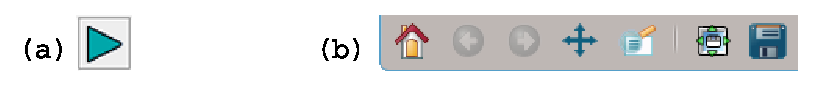
\includegraphics[width=10cm,clip=true,angle=0]{figures/refl_buttons.eps}
\caption[]{(a) `Run' button to start the Reflex workflow; (b) zoom toolbar
provided by the Python library {\tt matplotlib}. With the leftmost symbol, the
user always comes back to the overview; the second and the third symbol enables
the user to go `Back' and  `Forward' in the zooming history; the 4$^{\rm th}$
button shifts the plot via the mouse; the 5$^{\rm th}$ button is the actual
zooming button, which can be used via the mouse; the 6$^{\rm th}$ button opens a
window to configure the subplots; the 7$^{\rm th}$ button saves the plot to a
file.}
\label{fig:buttons}
\end{figure}

\begin{figure}
\centering
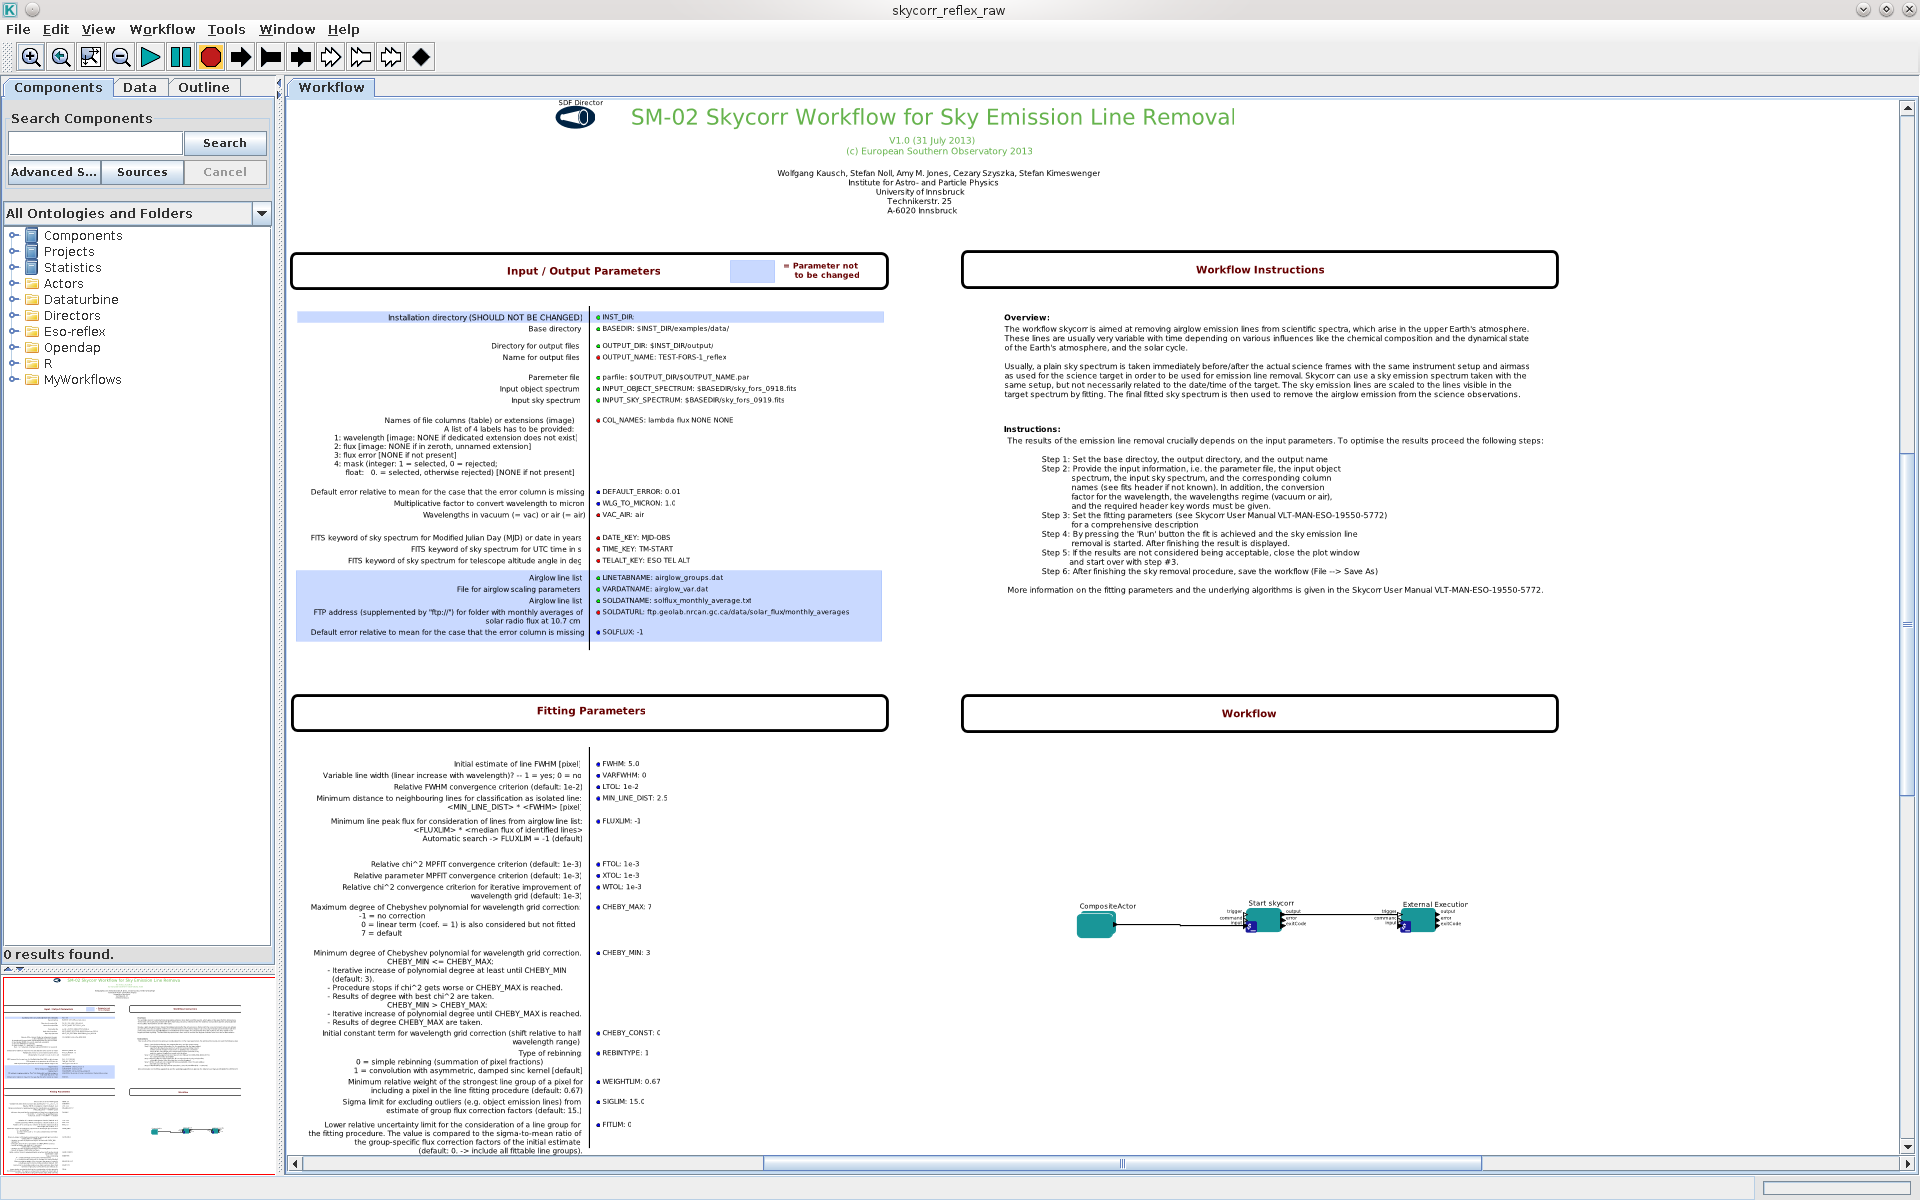
\includegraphics[width=21cm,clip=true,angle=-90]{figures/skycorr_reflex.png}
\caption[]{Canvas of the SKYCORR Reflex workflow.}
\label{fig:sc_reflex}
\end{figure}

\begin{figure}
\centering
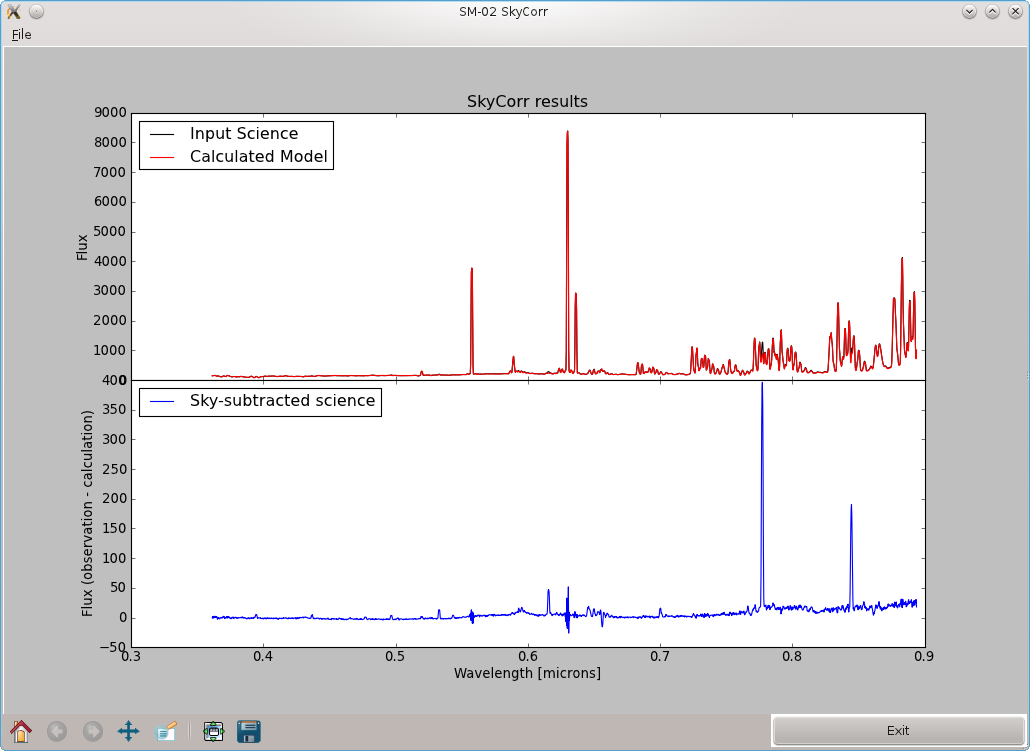
\includegraphics[width=17cm,clip=true,angle=-90]{figures/skycorr_gui.png}
\caption[]{Plot of the SKYCORR Reflex workflow.}
\label{fig:sc_gui}
\end{figure}


\cleardoublepage
%-------------------------------------------------------------------------------
\section{Mathematical / physical description}\label{sec:method}
%-------------------------------------------------------------------------------
In the following, we describe the SKYCORR sky correction procedure in more
detail (also see Section~\ref{sec:algorithm}). First, we discuss how emission
lines are identified in the input science and sky spectra
(Section~\ref{sec:linesearch}). This procedure also derives the typical line
FWHM (Section~\ref{sec:linesearch}). Next, the subtraction of the remaining
continua from the identified line spectra is described
(Section~\ref{sec:contsub}). Then, the airglow model is discussed
(Section~\ref{sec:airglow}). It is an essential input for scaling the
reference sky line spectrum to fit the science line spectrum
(Section~\ref{sec:linefit}). The fitting procedure also allows adapting the
wavelength grids (Section~\ref{sec:wavegrid}). The final step of the sky
correction procedure is the sky subtraction itself. This operation is just the
subtraction of the best-fit sky line spectrum and the unscaled sky continuum
spectrum from the input science spectrum (see also
Section~\ref{sec:algorithm}).

%-------------------------------------------------------------------------------
\subsection{Line finder}\label{sec:linesearch}
%-------------------------------------------------------------------------------
The sky correction procedure focuses on fitting the airglow emission lines in
an input science spectrum by scaling a reference sky line spectrum. Hence,
object and sky continua have to be subtracted in advance. This requires
identification of line and continuum pixels in the input spectra. Spectral
lines are identified by an approach that uses the first derivative of the
spectrum. Thus, line pixels can be recognised by their large flux gradients.
Emission line peaks can be identified by a change from positive to negative
values of the first derivative.

\begin{figure}
\centering
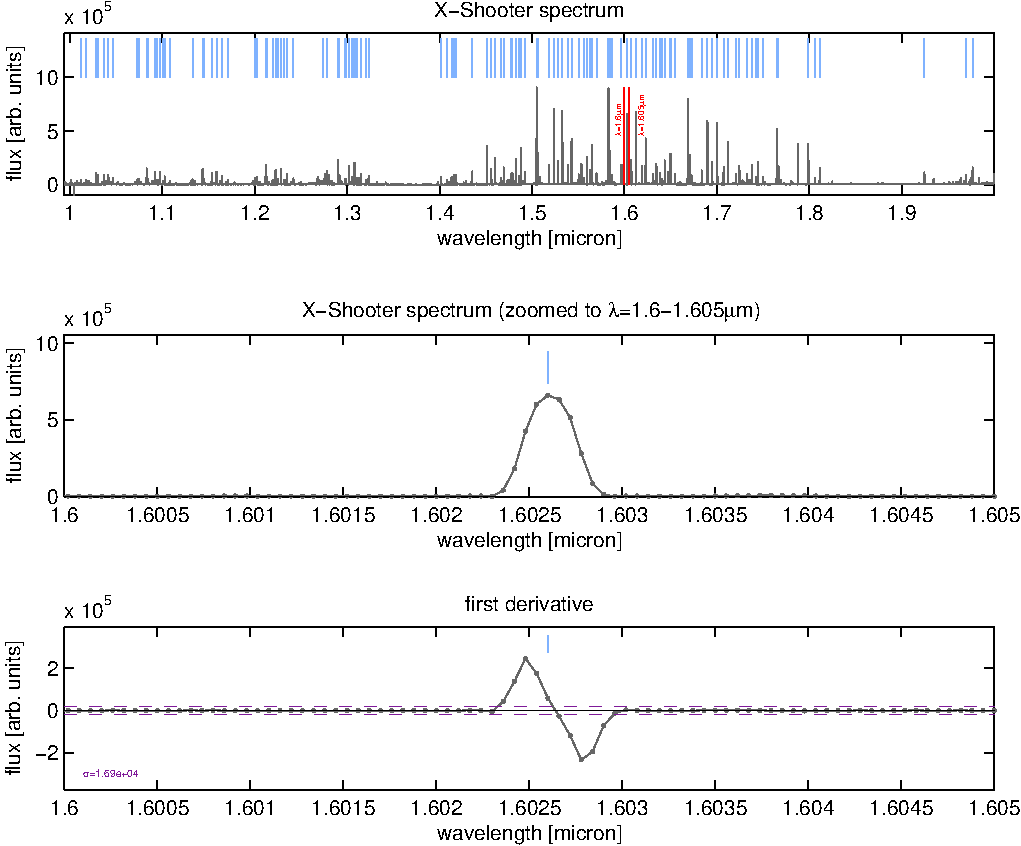
\includegraphics[width=17cm,clip=true]
{figures/X-Shooter_spec_deriv_1_6-1_605.pdf}
\caption[]{X-Shooter sky spectrum {\tt sky\_xshoo\_28}. The upper panel shows
the entire wavelength range $\lambda=1.0...2.0\,\mu$m with the zoom range
$\lambda=1.6...1.605\,\mu$m (red lines) shown in the middle panel containing a
prominent single emission line. In the lower panel the first derivative of this
line is given, which shows a significant change in the values. Such changes
are used as signature to identify emission lines (marked by the light blue
vertical lines in the panels).}
\label{fig:xshoo1}
\end{figure}

\begin{figure}
\centering
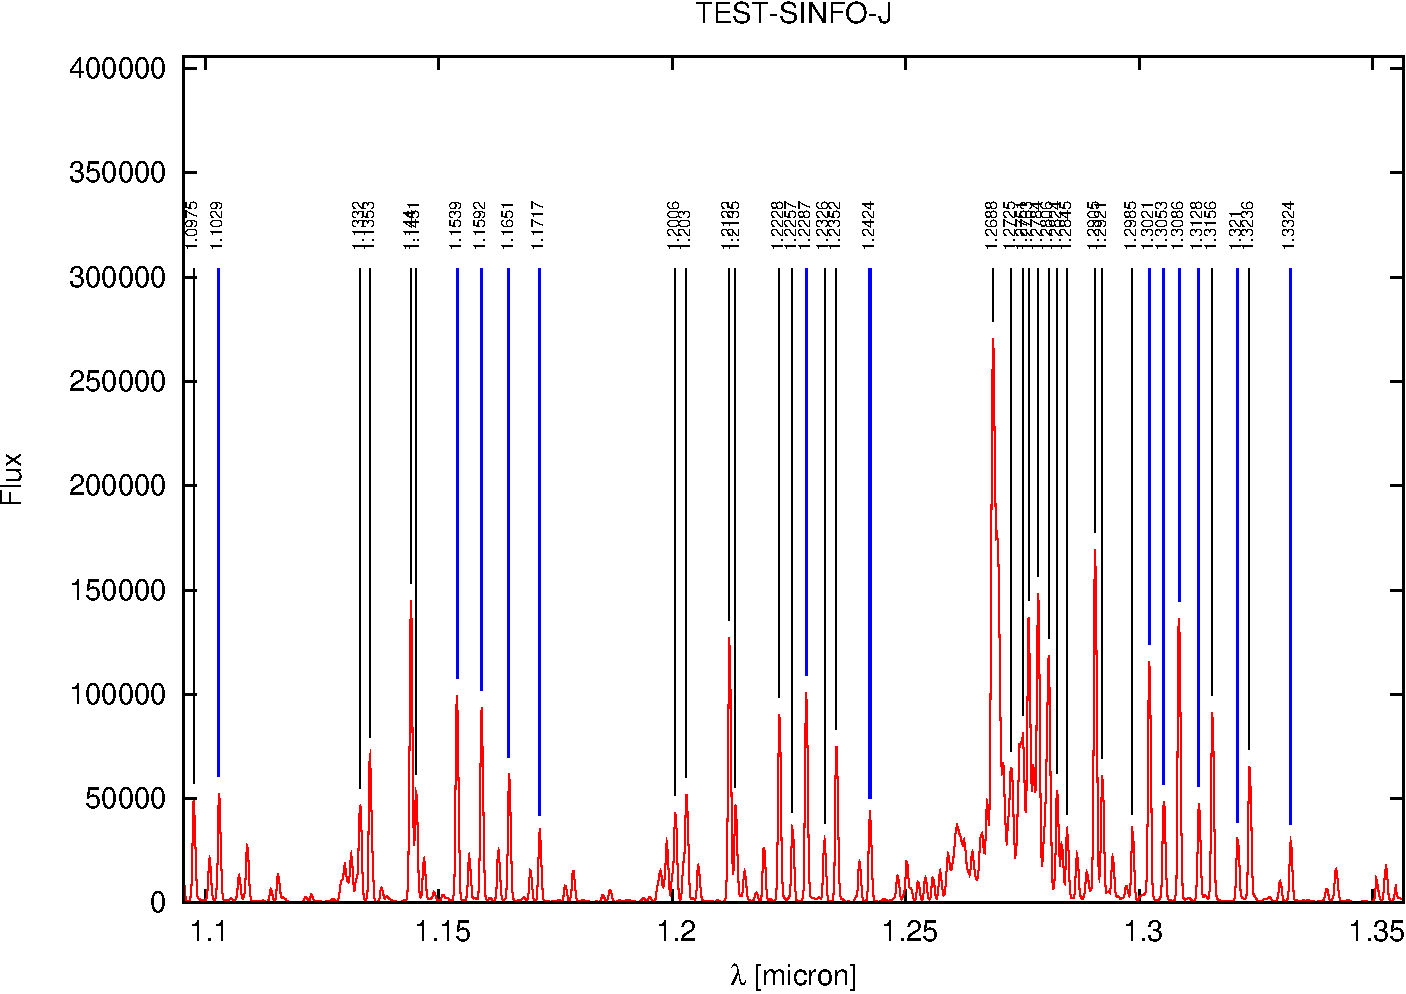
\includegraphics[width=9.5cm,clip=true]
{figures/TEST-SINFO-J_with_lines.pdf}
\caption[]{SINFONI $J$-band sky spectrum with detected emission lines
(blue = isolated lines used for the FWHM estimate).}
\label{fig:sinfoj1}
\end{figure}

\begin{figure}
\centering
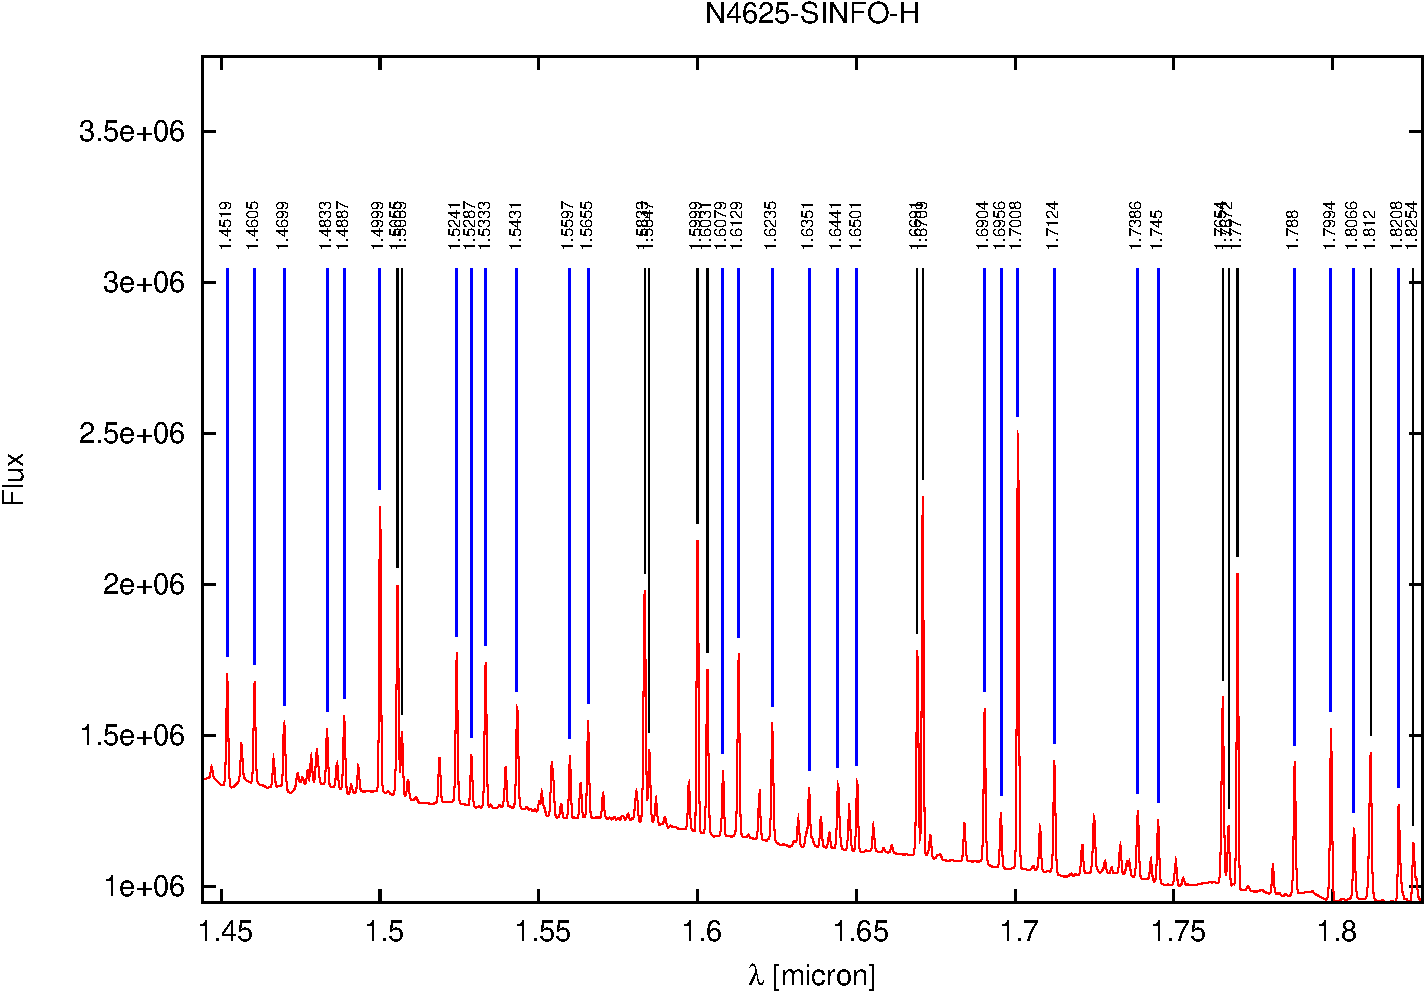
\includegraphics[width=9.5cm,clip=true]
{figures/N4625-SINFO-H_with_lines.pdf}
\caption[]{SINFONI $H$-band sky spectrum + arbitrarily scaled NGC\,4625
spectrum at $z = 0.5$ + 5 artificial emission lines of equal intensity with
detected emission lines (blue = isolated lines used for the FWHM estimate).}
\label{fig:sinfoh1}
\end{figure}

Figure~\ref{fig:xshoo1} shows the X-Shooter spectrum {\tt sky\_xshoo\_28} (see
Section~\ref{sec:evaluation}) in the upper panel. A zoom-in to the wavelength
range $\lambda=1.6...1.605\,\mu$m isolates a prominent single emission line
(middle panel). The first derivative of the same spectral range (lower panel)
reveals a significant change from positive to negative values allowing
detection of emission lines. Single emission lines are identified by this
particular signature. Note that only changes $\geq1\sigma$ above the noise
level are taken into account to avoid spurious detections from noise or broad
lines caused by blending.

Line identification via the first derivative allows robust characterisation of
lines also in case of strong (pseudo)\-continuum variations. This is necessary
as isolated lines are required for estimating their FWHM.
Figures~\ref{fig:sinfoj1} and \ref{fig:sinfoh1} show a SINFONI $J$-band and
$H$-band spectrum, respectively. In the latter a simulated object
spectrum was added to the sky emission (see Section~\ref{sec:evaluation} for
more information). The distinct emission peak at $\lambda\sim1.25....1.3\,\mu$m
in the $J$-band is a pseudocontinuum caused by many unresolved O$_2$ sky lines,
whereas in the $H$-band observation a real continuum is visible. In both cases,
individual emission lines could be identified.

All detected lines are assembled in a line list, which is refined by an
iterative method depending on the estimation of the sky line FWHM (see
Section~\ref{sec:FWHM}). This procedure requires identification of strong,
isolated lines. Therefore, the line finder checks the previously identified
line peaks, applying criteria characterising isolated lines. For a line to be
marked as isolated, it has to be sufficiently separated from other lines and
its peak has to have a symmetric shape. The first criterion can be influenced
by the user. The parameter file includes the unitless scaling parameter {\sc
min\_line\_dist} that is internally multiplied by the line FWHM in pixels.
Also, this parameter is included in the driver file (see
Section~\ref{sec:params}). Since the FWHM is optimised in an iterative
procedure (see Section~\ref{sec:FWHM}), the given value in the file is only
used as first guess.

For strong and well separated lines, the described line finding method is very
robust. However, for low resolution spectra with many blended lines a major
fraction of lines may be missed. Therefore, the line list of the airglow model
is being used (see Section~\ref{sec:airglow}) to find previously unidentified
lines that have fluxes above the median flux of the lines identified by the
derivative approach times the {\sc fluxlim} parameter of the parameter file. By
default, {\sc fluxlim} is set to -1, which indicates an iterative approach
starting with 0.005 and doubling the previous value in subsequent iterations.
If the higher limit does not spare sufficient continuum pixels for the
continuum interpolation (see Section~\ref{sec:contsub}), \ie\ at least 20\% of
all pixels distributed over more than 90\% of the wavelength range, the
procedure is stopped and 0.005 is eventually selected, otherwise the threshold
value is doubled (\ie\ 0.02 is taken). This process is repeated as long as a
sufficient number of continuum pixels are left over or a value of 0.08 is
reached. The number of pixels characterised as line pixels for each line
included from the line list depends on the given line FWHM (see above and
Section~\ref{sec:FWHM}). The combination of line pixels identified by both
methods gives a good estimate of the spectral ranges covered by significant
airglow lines (see Figure~\ref{fig:lineflags}).

\begin{figure}
\centering
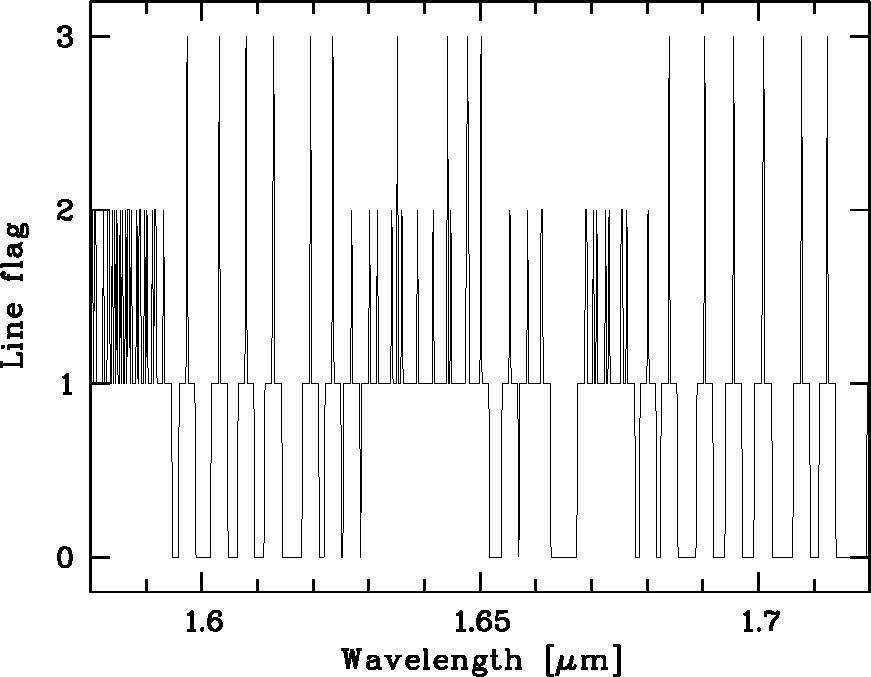
\includegraphics[width=12cm,clip=true]{figures/scd_illlineflags.pdf}
\caption[]{Line flags identified in a part of a SINFONI $H$-band spectrum. The
meaning of the flags is as follows: 0 = continuum, 1 = line pixel,
2 = line peak, 3 = isolated line peak.}
\label{fig:lineflags}
\end{figure}

%-------------------------------------------------------------------------------
\subsection{Line FWHM estimator}\label{sec:FWHM}
%-------------------------------------------------------------------------------
For calculating the airglow model (see Section~\ref{sec:airglow}), it is
required to convert total line fluxes as provided by the input line list into
fluxes per wavelength interval. Consequently, it is necessary to know the
typical FWHM of the airglow lines, which is the only line shape parameter
assuming a Gaussian line profile. The line finder described in the previous
Section~\ref{sec:linesearch} searches for isolated lines that are suitable for
deriving a FWHM. After the subtraction of the continuum (see
Section~\ref{sec:contsub}), the FWHM estimation can be performed by fitting a
Gaussian to the line pixels belonging to each isolated line. For the fitting
procedure, the C version of the least-squares fitting library MPFIT by
C.~Markwardt~\cite{CMPFIT} based on the FORTRAN fitting routine MINPACK-1 by
Mor\'e et al.~\cite{MOR80} is used (see also Section~\ref{sec:linefit}).
The FWHM measurements of all isolated lines are averaged to obtain the typical
FWHM of the input spectrum. In order to avoid blended lines contributing to
the resulting mean, a $\sigma$-clipping approach is applied to skip
suspiciuosly high FWHM. The method is based on computing the median absolute
difference between the data points and their median and the subsequent
application of Huber's method for an iterative clipping of outliers
\cite{huber} and the derivation of reliable mean and standard deviation from
the unclipped values. If less than five isolated lines remain after clipping,
the median FWHM is taken.

The fact that the estimated value of the FWHM affects the search for isolated
lines (see Section~\ref{sec:linesearch}), which are required for the FWHM
estimation, necessitates an iterative approach in which line finder, continuum
subtractor, and FWHM estimator are called several times in turn in order to
obtain a stable and trustworthy FWHM. This iterative procedure is terminated if
convergence is reached for the mean FWHM. The convergence criterion is
provided by the parameter {\sc ltol} (see Section~\ref{sec:params}).

For instruments like X-Shooter, whose spectra show a roughly linear increase of
the FWHM with wavelength, this can be considered by the setting the parameter
{\sc varfwhm} to 1. In this case, the FWHM estimates of the individual lines
are converted to correspond to the FWHM, which would be measured at the
central wavelength of the full spectrum, assuming a linear change of the
FWHM with wavelength. The converted FWHM are then used to calculate the mean
FWHM as discussed above. The linear change of the FWHM is also considered for
the separation of lines and continuum (see Section~\ref{sec:linesearch}) and
the calculation of the pixel contributions of the different line groups
(see Section~\ref{sec:linefit}).

%-------------------------------------------------------------------------------
\subsection{Continuum subtraction}\label{sec:contsub}
%-------------------------------------------------------------------------------
\begin{figure}
\centering
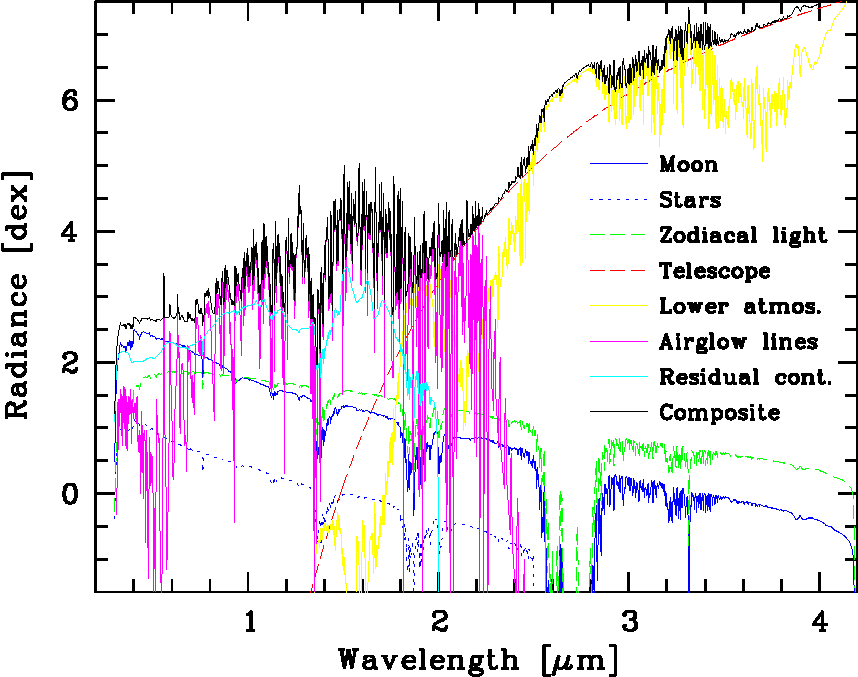
\includegraphics[width=12cm,clip=true]{figures/smd2_logcomp.pdf}
\caption[]{Components of the SM-01 sky model for wavelengths between $0.3$ and
6\,$\mu$m in logarithmic flux units. The example with Moon above the horizon
shows the scattered moonlight, scattered starlight, zodiacal light, thermal
emission by telescope and instrument, molecular emission of the lower
atmosphere, airglow emission lines of the upper atmosphere, and
airglow/residual continuum.}
\label{fig:logcomp}
\end{figure}

The adaptation of the reference sky line spectrum to the airglow lines in the
input science spectrum by multiplying factors to physically motivated line
groups (see Section~\ref{sec:airglow}) requires that any kind of continuum is
subtracted before this procedure. In particular, the object continuum can cause
problems, since it is not present in the reference sky spectrum. However, sky
spectra also show continuum emission. The main components are scattered
moonlight, scattered starlight, zodiacal light, thermal emission from the lower
atmosphere by greenhouse gases and the telescope itself, and airglow continuum
emission, which is related most probably to chemiluminescent reactions in the
upper atmosphere involving nitric oxide (see Section~\ref{sec:airglow}, Noll et
al.~\cite{NOL12}, and Khomich et al.~\cite{KHO08} and references therein). As
Figure~\ref{fig:logcomp} indicates, the main continuum component is the
airglow/residual continuum\footnote{Note that this component is very difficult
to determine. Its measured intensity strongly depends on the accuracy of the
other components, the quality of the flux calibration, and possible
instrumental continua. For this reason, it should also been seen as residual
continuum.}, which dominates shortwards of the thermal regime with the
exception of the UV and optical if the Moon is up. The variable airglow
continuum (see Figure~\ref{fig:illfeatvar}) cannot be corrected by a fitting
procedure like for the airglow lines (see Section~\ref{sec:airglow}), since
object and sky continuum cannot be separated in the science spectrum (cf.
Section~\ref{sec:davies}). Therefore, it has to be assumed that the sky
continuum in the science spectrum does not differ much from the one in the
reference sky spectrum. If this requirement is fulfilled, a simple subtraction
of the continua in both input spectra of the sky correction procedure should
provide results with good quality.

SKYCORR obtains the continua in the input science and sky spectra using line
identification flags (see Figure~\ref{fig:lineflags}) set in the course of the
line search described in Section~\ref{sec:linesearch}. All pixels not flagged
as line pixels are connected by linear interpolation. Thorough identification
of continuum pixels guaranteed, this is the most efficient approach even in the
case of line blends covering wide wavelength ranges.

%-------------------------------------------------------------------------------
\subsection{Airglow model}\label{sec:airglow}
%-------------------------------------------------------------------------------
\begin{figure}
\centering
\includegraphics[width=10cm,clip=true]{figures/varclasses.eps}
\caption[]{Variability classes for sky emission lines. The following groups are
defined: green O\,I, Na\,I\,D, red O\,I, OH, and O$_2$. The weak lines (green
curves) are scaled by a factor of 30 for Na\,I\,D, red O\,I, and O$_2$, and a
factor of 10 for OH.}
\label{fig:varclasses}
\end{figure}

\begin{figure}
\centering
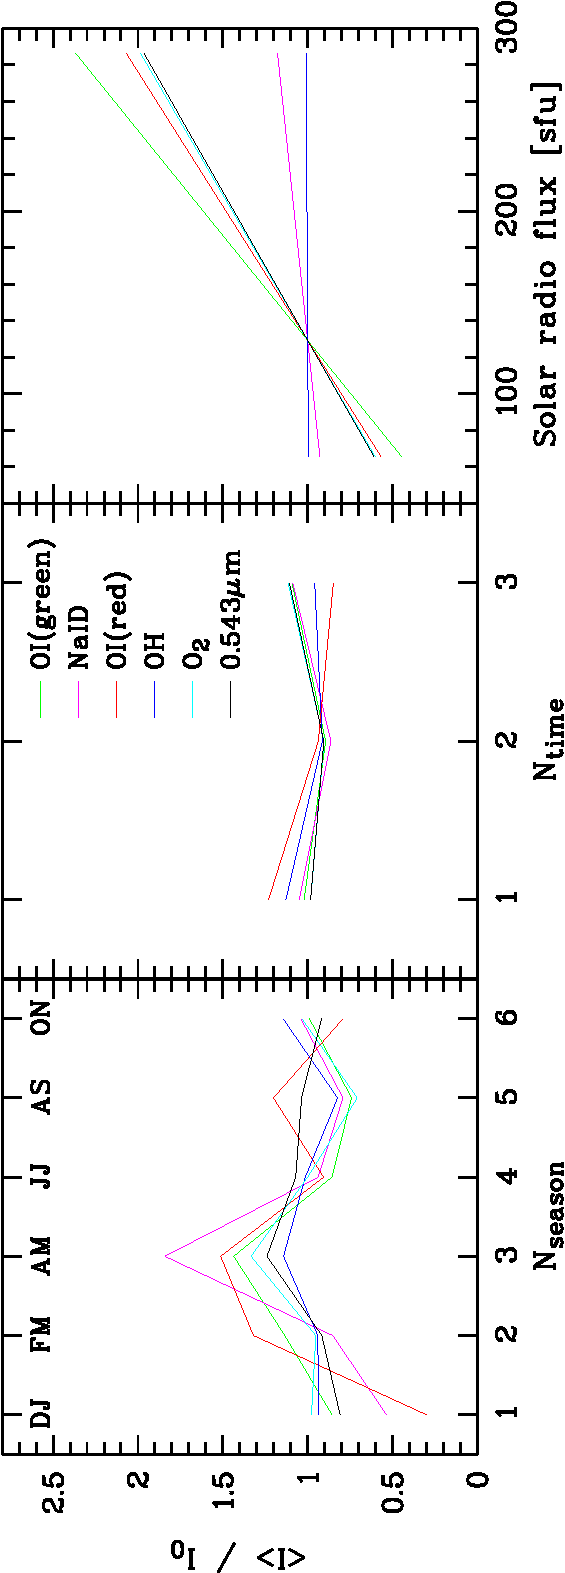
\includegraphics[height=\textwidth,angle=-90,clip=true]
{figures/scd_illfeatvar.pdf}
\caption[]{Variability correction for the five sky line classes and the
airglow continuum of the sky model. The variability is shown as a function of
the bimonthly period (1 = Dec/Jan, ..., 6 = Oct/Nov), time bin (third of the
night), and the solar activity measured by the solar radio flux
(sfu~$= 0.01$\,MJy).}
\label{fig:illfeatvar}
\end{figure}

\begin{table}
\caption[]{Description of A groups in the input line list}
\label{tab:Agroups}
\centering
\footnotesize
\vspace{5pt}
\begin{tabular}{c c c l}
\hline\hline
\noalign{\smallskip}
ID & $N_\mathrm{lin}$ & Wavelength range [\mum] & Description \\
\noalign{\smallskip}
\hline
\noalign{\smallskip}
 1 &  61 & 0.314 - 0.872 & green O\,I at 0.5577\,$\mu$m + unidentified lines \\
 2 &   3 & 0.589 - 0.770 & Na\,I\,D + other lines from alkali metals \\
 3 &  23 & 0.389 - 0.845 & red O\,I at 0.6300\,$\mu$m + other thermospheric
                           lines \\
 4 &   1 & 0.467 - 0.467 & OH(7-0) \\
 5 &   8 & 0.491 - 0.495 & OH(8-1) \\
 6 &  22 & 0.519 - 0.536 & OH(9-2) \\
 7 &  12 & 0.526 - 0.535 & OH(6-0) \\
 8 &  23 & 0.554 - 0.570 & OH(7-1) \\
 9 &  41 & 0.587 - 0.634 & OH(8-2) \\
10 &  49 & 0.624 - 0.655 & OH(9-3) \\
11 &   2 & 0.672 - 0.674 & OH(10-4) \\
12 &  27 & 0.614 - 0.695 & OH(5-0) \\
13 &  83 & 0.647 - 0.754 & OH(6-1) \\
14 & 113 & 0.681 - 0.782 & OH(7-2) \\
15 & 111 & 0.720 - 0.815 & OH(8-3) \\
16 &  72 & 0.768 - 0.822 & OH(9-4) \\
17 &   7 & 0.827 - 0.839 & OH(10-5) \\
18 &  85 & 0.745 - 0.910 & OH(4-0) \\
19 & 113 & 0.781 - 0.914 & OH(5-1) \\
20 & 111 & 0.826 - 0.916 & OH(6-2) \\
21 & 110 & 0.873 - 0.937 & OH(7-3) \\
22 & 116 & 0.931 - 1.007 & OH(8-4) \\
23 & 120 & 0.994 - 1.081 & OH(9-5) \\
24 & 100 & 0.965 - 1.043 & OH(3-0) \\
25 & 110 & 1.015 - 1.098 & OH(4-1) \\
26 & 112 & 1.069 - 1.168 & OH(5-2) \\
27 & 118 & 1.129 - 1.236 & OH(6-3) \\
28 & 120 & 1.197 - 1.314 & OH(7-4) \\
29 & 124 & 1.275 - 1.420 & OH(8-5) \\
30 & 128 & 1.366 - 1.531 & OH(9-6) \\
31 & 112 & 1.392 - 1.558 & OH(2-0) \\
32 & 118 & 1.461 - 1.654 & OH(3-1) \\
33 & 122 & 1.537 - 1.743 & OH(4-2) \\
34 & 122 & 1.622 - 1.842 & OH(5-3) \\
35 & 124 & 1.717 - 1.978 & OH(6-4) \\
36 & 126 & 1.825 - 2.110 & OH(7-5) \\
37 & 130 & 1.951 - 2.265 & OH(8-6) \\
38 & 130 & 2.101 - 2.454 & OH(9-7) \\
39 & 450 & 0.314 - 0.532 & O$_2$(A-X) (Herzberg I) \\
40 &   5 & 0.324 - 0.410 & O$_2$(c-X) (Herzberg II) \\
41 & 396 & 0.326 - 0.550 & O$_2$(A'-a) (Chamberlain) \\
42 &  65 & 0.382 - 0.509 & O$_2$(c-b) \\
43 & 208 & 0.656 - 0.806 & O$_2$(b-X) (v' > v'') \\
44 & 194 & 0.761 - 0.816 & O$_2$(b-X) (v' = v'') \\
45 & 103 & 0.861 - 0.922 & O$_2$(b-X) (v' < v''; atmospheric 0-1 band
                           inclusive) \\
46 & 161 & 1.240 - 1.305 & O$_2$(a-X)(0-0) (IR atmospheric system) \\
47 &  73 & 1.555 - 1.598 & O$_2$(a-X)(0-1) (IR atmospheric system) \\
\noalign{\smallskip}
\hline
\end{tabular}
\end{table}

\begin{table}
\caption[]{Description of B groups in the input line list}
\label{tab:Bgroups}
\centering
\footnotesize
\vspace{5pt}
\begin{tabular}{c c l l}
\hline\hline
\noalign{\smallskip}
ID & Molecule & Upper state(s) & Remarks$^\mathrm{a}$ \\
\noalign{\smallskip}
\hline
\noalign{\smallskip}
 1 & OH & $X^2\Pi_{1/2}$, $J' = 1/2$  & Q2(0.5), P2(1.5) \\
 2 & OH & $X^2\Pi_{3/2}$, $J' = 3/2$  & Q1(1.5), P1(2.5) \\
 3 & OH & $X^2\Pi_{1/2}$, $J' = 3/2$  & R2(0.5), Q2(1.5), P2(2.5) \\
 4 & OH & $X^2\Pi_{3/2}$, $J' = 5/2$  & R1(1.5), Q1(2.5), P1(3.5) \\
 5 & OH & $X^2\Pi_{1/2}$, $J' = 5/2$  & R2(1.5), Q2(2.5), P2(3.5) \\
 6 & OH & $X^2\Pi_{3/2}$, $J' = 7/2$  & R1(2.5), Q1(3.5), P1(4.5) \\
 7 & OH & $X^2\Pi_{1/2}$, $J' = 7/2$  & R2(2.5), Q2(3.5), P2(4.5) \\
 8 & OH & $X^2\Pi_{3/2}$, $J' = 9/2$  & R1(3.5), Q1(4.5), P1(5.5) \\
 9 & OH & $X^2\Pi_{1/2}$, $J' = 9/2$  & R2(3.5), Q2(4.5), P2(5.5) \\
10 & OH & $X^2\Pi_{3/2}$, $J' = 11/2$ & R1(4.5), Q1(5.5), P1(6.5) \\
11 & O$_2$ & $b^1\Sigma^+_g$, $J' = 0, 2, 4$ & \\
12 & O$_2$ & $b^1\Sigma^+_g$, $J' = 6, 8$ & \\
13 & O$_2$ & $b^1\Sigma^+_g$, $J' = 10, 12$ & \\
14 & O$_2$ & $b^1\Sigma^+_g$, $J' = 14, 16$ & \\
15 & O$_2$ & $a^1\Delta_g$, $J' = 2, 4$ & $v'' = 0$ \\
16 & O$_2$ & $a^1\Delta_g$, $J' = 6, 8$ & $v'' = 0$ \\
17 & O$_2$ & $a^1\Delta_g$, $J' = 10, 12$ & $v'' = 0$ \\
18 & O$_2$ & $a^1\Delta_g$, $J' = 14, 16$ & $v'' = 0$ \\
19 & O$_2$ & $a^1\Delta_g$, $J' = 18, 20$ & $v'' = 0$ \\
20 & O$_2$ & $a^1\Delta_g$, $J' = 20, 22$ & $v'' = 0$ \\
21 & O$_2$ & $a^1\Delta_g$, $J' = 2, 4$ & $v'' \ne 0$ \\
22 & O$_2$ & $a^1\Delta_g$, $J' = 6, 8$ & $v'' \ne 0$ \\
23 & O$_2$ & $a^1\Delta_g$, $J' = 10, 12$ & $v'' \ne 0$ \\
24 & O$_2$ & $a^1\Delta_g$, $J' = 14, 16$ & $v'' \ne 0$ \\
\noalign{\smallskip}
\hline
\end{tabular}
\footnotesize
\begin{list}{}{}
\item[$^\mathrm{a}$] OH rotational transitions or lower vibrational level for
O$_2$(a-X) transitions
\end{list}
\end{table}

\begin{figure}
\centering
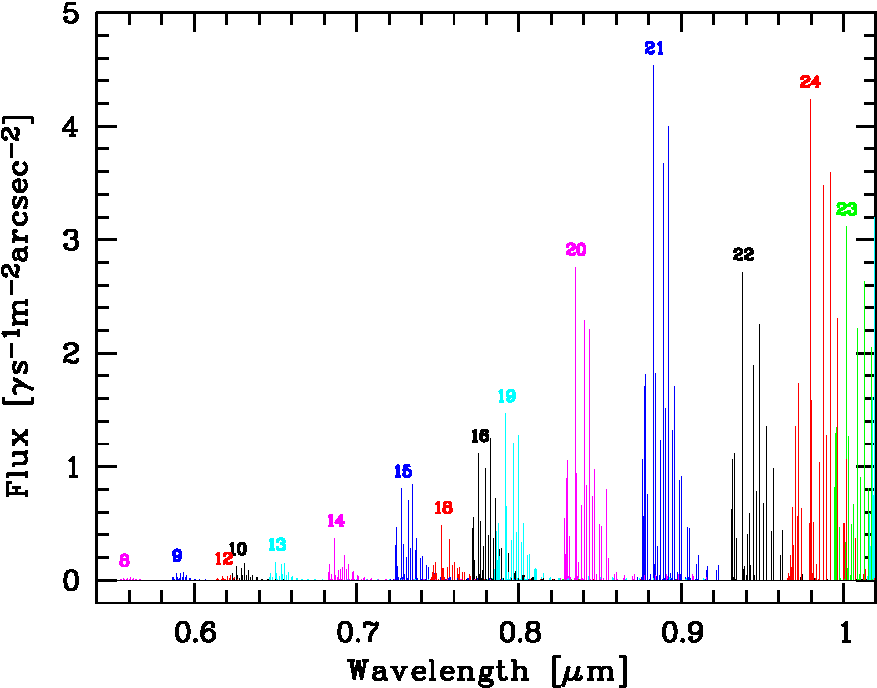
\includegraphics[width=10cm,clip=true]
{figures/scd_plotohbands_opt.pdf}
\caption[]{A group identifications of OH bands (cf. Table~\ref{tab:Agroups}) in
the wavelength range between 0.54 and 1.02\,\mum{} that have Q1(1.5) lines
(see Table~\ref{tab:Bgroups} and Figure~\ref{fig:ohband}) stronger than
0.01\,$\gamma\,{\rm s}^{-1}\,{\rm m}^{-2}\,{\rm arcsec}^{-2}$. The wavelengths and
zenithal mean fluxes (considering absorption in the lower atmosphere) tabulated
in the input line list are plotted. Note that the bands with numbers up to 21
appear twice as strong as the bands at longer wavelengths, since the
corresponding lines were taken from the Hanuschik \cite{HAN03} atlas, where OH
doublets are often unresolved and are listed as one line only.}
\label{fig:ohbands_opt}
\end{figure}

\begin{figure}
\centering
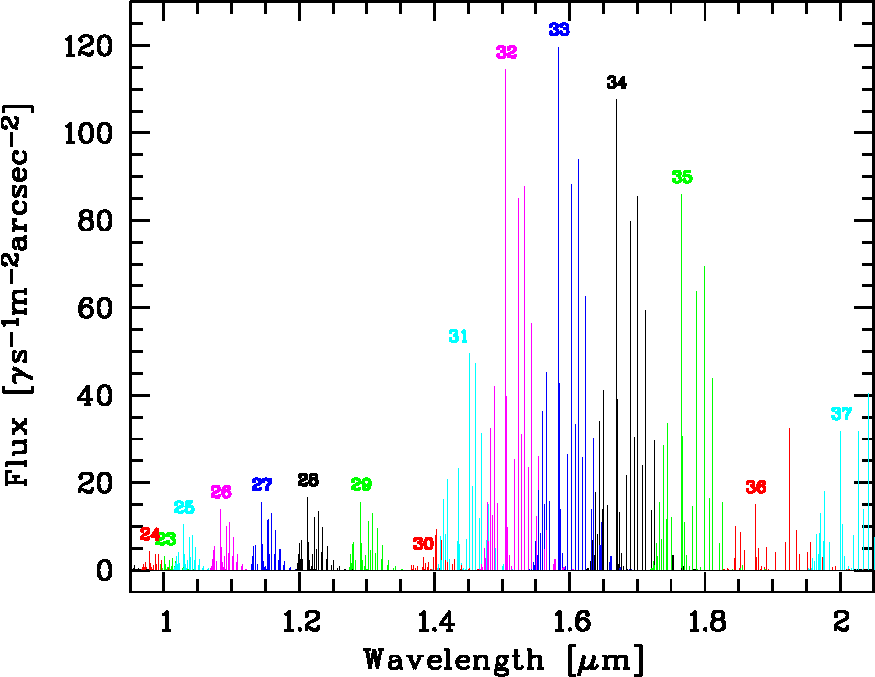
\includegraphics[width=10cm,clip=true]
{figures/scd_plotohbands_ir.pdf}
\caption[]{A group identifications of the OH bands (cf.
Table~\ref{tab:Agroups}) in the wavelength range between 0.95 and 2.05\,\mum{}.
The wavelengths and zenithal mean fluxes tabulated in the input line list are
plotted.}
\label{fig:ohbands_ir}
\end{figure}

\begin{figure}
\centering
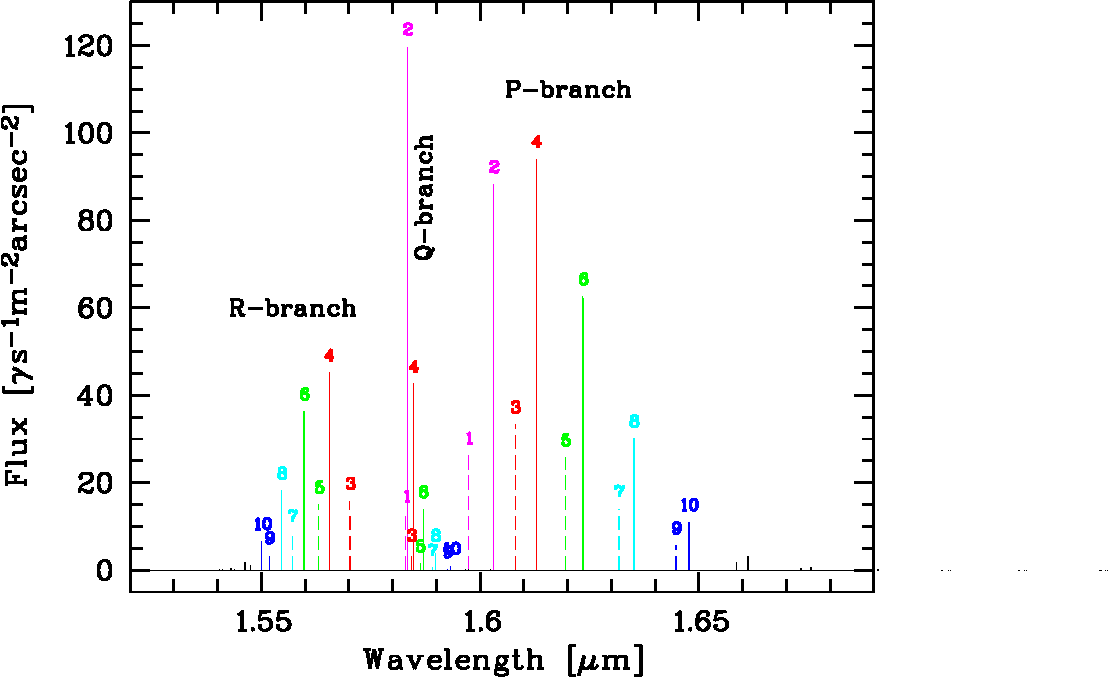
\includegraphics[width=10cm,clip=true]
{figures/scd_plotohband.pdf}
\caption[]{B group identifications of the transitions of an OH band with the
same rotational upper state (cf. Table~\ref{tab:Bgroups}). The tabulated
wavelengths and zenithal mean fluxes of the lines of the OH(6-4) band are shown
as example. Dashed and solid lines indicate transitions of the $X^2\Pi_{1/2}$ and
$X^2\Pi_{3/2}$ state, respectively. The figure also indicates the R-, Q-, and
P-branches that correspond to transitions with a change of the total angular
momentum by -1, 0, and 1, respectively.}
\label{fig:ohband}
\end{figure}

\begin{figure}
\centering
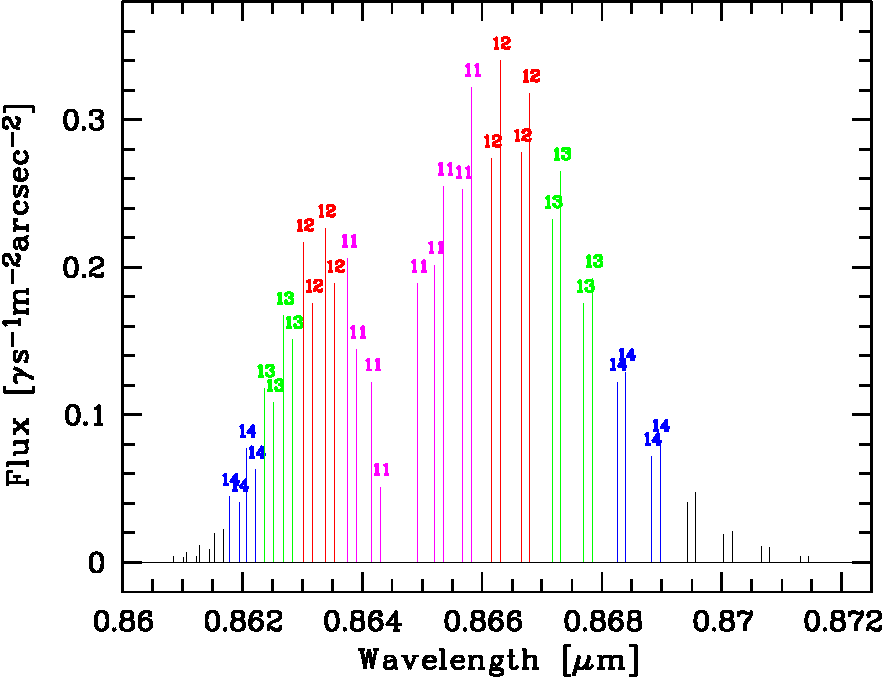
\includegraphics[width=10cm,clip=true]
{figures/scd_ploto2b01band.pdf}
\caption[]{B group identifications of the transitions of the band
O$_2$(b-X)(0-1) with a similar rotational upper state (cf.
Table~\ref{tab:Bgroups}). The tabulated wavelengths and zenithal mean fluxes of
the lines of the 4 different branches (2 R- and 2 P-branches) are shown (cf.
Figure~\ref{fig:ohband}).}
\label{fig:o2b01band}
\end{figure}

\begin{figure}
\centering
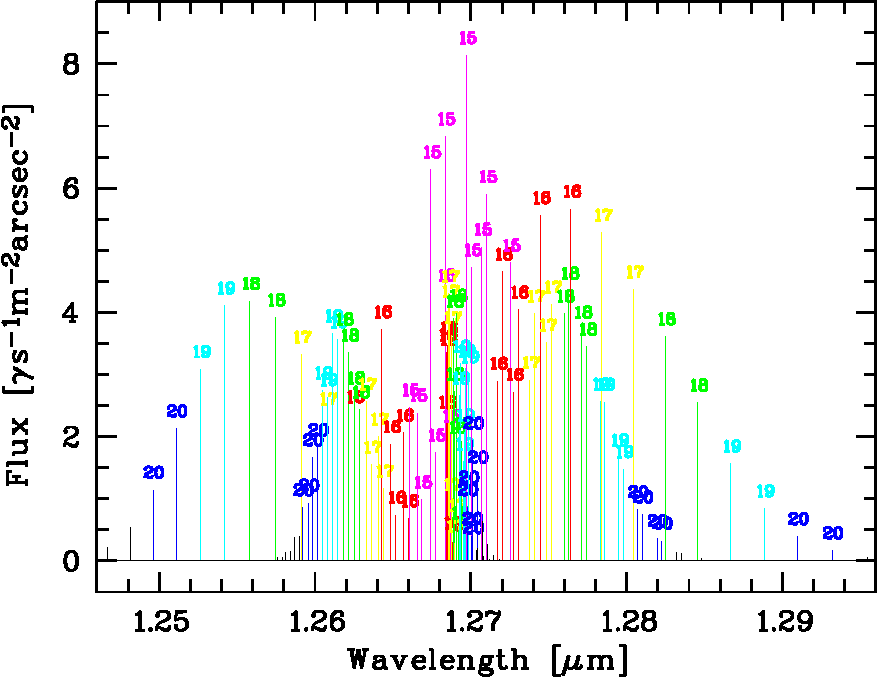
\includegraphics[width=10cm,clip=true]
{figures/scd_ploto2a00band.pdf}
\caption[]{B group identifications of the transitions of the band
O$_2$(a-X)(0-0) with a similar rotational upper state (cf.
Table~\ref{tab:Bgroups}). The tabulated wavelengths and zenithal mean fluxes of
the lines of the 9 different branches (3 R-, 3 Q-, and 3 P-branches) are shown
(cf. Figure~\ref{fig:ohband}). The band is strongly affected by self
absorption in the lower atmosphere.}
\label{fig:o2a00band}
\end{figure}

\begin{figure}
\centering
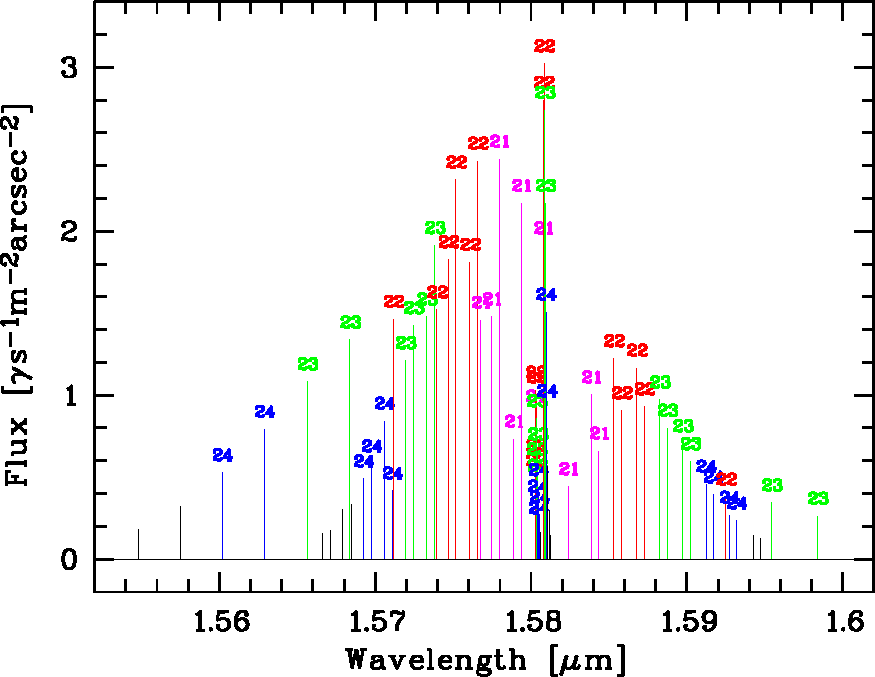
\includegraphics[width=10cm,clip=true]
{figures/scd_ploto2a01band.pdf}
\caption[]{B group identifications of the transitions of the band
O$_2$(a-X)(0-1) with a similar rotational upper state (cf.
Table~\ref{tab:Bgroups}). The tabulated wavelengths and zenithal mean fluxes of
the lines of the 9 different branches (3 R-, 3 Q-, and 3 P-branches) are shown
(cf. Figure~\ref{fig:ohband}).}
\label{fig:o2a01band}
\end{figure}

The wavelength range from the near-UV to the near-IR is characterised by strong
emission lines. Most of them constitute band structures. This airglow (see
Khomich et al.~\cite{KHO08} for a comprehensive discussion) mostly originates
in the mesopause region at about 90\,km. In addition, some lines arise in the
ionospheric F2-layer at about 270\,km. In general, airglow is caused by
chemiluminescence, \ie\ chemical reactions that lead to light emission by the
decay of excited electronic states of reaction products. Apart from atomic
oxygen and sodium, the oxygen (O$_2$) and hydroxyl (OH) molecules are the most
important reaction products in this context. In general, airglow lines show
strong variability from time scales in the order of minutes to years. This
behaviour can be explained by the solar activity cycle, seasonal changes in
temperature, pressure, and chemical composition of the emission layers, the
day-night contrast, dynamical effects such as gravity waves, or geomagnetic
disturbances.

The SKYCORR project aims at correcting airglow emission in science spectra by
means of reference sky spectra taken at a different time. As the airglow is
highly variable, the strength of the emission lines in a reference spectrum has
to be adapted, though. This is achieved by a fitting procedure that is
discussed in Section~\ref{sec:linefit}. Since emission lines belonging to the
science target should not be reproduced by the optimised sky spectrum and
finally removed, it is advisable to adapt as many lines as possible by a
single fitting parameter. Every group should contain airglow lines that are not
affected by object lines and that can be used to determine a realistic
correction factor for the reference sky spectrum. The number of lines that can
be combined is limited by the fact that they should show an almost identical
variability behaviour.

As basis for the definition of suitable line groups, the airglow line model
developed in the course of the SM-01 project for an advanced sky background
model for \ac{ESO} exposure time calculators was used (see \cite{SM01} User
Manual; Noll et al.~\cite{NOL12}). This semi-empirical model consists of a line
list with line intensities for mean observing conditions and prescriptions for
the correction of the line strength depending on molecular species, solar
activity, season, night time, and zenith distance of the target. The latter
three input parameters can be retrieved from the \ac{FITS} header of the sky
spectrum file. The solar activity is provided as solar radio flux at 10.7\,cm
either directly by {\sc solflux} in the parameter file or by the corresponding
monthly average (default) in a file offered by {\tt www.spaceweather.gc.ca}
(see Section~\ref{sec:params}). In the wavelength range from $0.3143$ to
$0.9228$\,\mum{}, the line list consists of data taken from Cosby et
al.~\cite{COS06} (supplemented by unpublished UVES 800U data) who incorporated
the UVES-based sky emission line atlas of Hanuschik \cite{HAN03}. At longer
wavelengths the calculated OH lines of Rousselot et al.~\cite{ROU00} were
included. However, their line strengths were corrected for the Einstein factors
of Goldman et al.~\cite{GOL98} instead of using the original, outdated ones of
Mies~\cite{MIE74}. This resulted in correction factors for OH band strengths
between 0.38 and 2.06. Moreover, the flux decrease of airglow lines by
molecular absorption in the lower atmosphere was corrected by the
multiplication of the airglow line spectrum with Doppler line widths for
typical temperatures of about 200\,K by the high-resolution
($\lambda / \Delta\lambda \approx 10^6$) Paranal annual-mean transmission
curve for an airmass of 1.25\footnote{Although the atmospheric
transmission depends on airmass and weather conditions, only a fixed airglow
flux correction was applied in order to avoid time-consuming calculations at
very high resolution and the input of temperature and water vapour profiles.
Moreover, the optical airglow atlas of Hanuschik \cite{HAN03} is also
characterised by a fixed transmission correction due to the use of UVES mean
spectra. For most observing conditions, the deviation of the true airglow
absorption from the assumed one is expected to be minor in terms of the results
of SKYCORR.} (see Noll et al. \cite{NOL12}). The transmission curve was
computed by means of the radiative transfer code LBLRTM (see Clough et al.
\cite{CLO05} and \cite{LBLRTM}). Note that SKYCORR applies the Paranal mean
transmission curve for zenith (corrected for the target airmass) to the
unextincted fluxes in the input line list. For this purpose, the line list
contains separate columns for unextincted line fluxes and zenithal transmission
values. Finally, the Rousselot et al.~lines were scaled to the Cosby et
al.~lines between $0.642$ and $0.858$\,\mum{}. The strongest O$_2$ bands in the
near-IR at $1.27$ and $1.58$\,\mum{} were included in the line list by adding
data from the HITRAN database (see Rothman et al.~\cite{ROT09} and
\cite{HITRAN}). The mean band strength was roughly estimated evaluating the
ratio of O$_2$ to OH lines in 26 IR X-Shooter spectra. For this purpose, the
O$_2$ lines had to be extincted depending on the airmass values of the
X-Shooter spectra. In the case of the $1.27$\,\mum{} band, this caused
significant changes in the line fluxes due to the strong resonant absorption of
airglow photons by tropospheric/stratospheric O$_2$ molecules in the ground
state.

The SM-01 sky model assigns the listed lines to five different variability
classes (see Figure~\ref{fig:varclasses}). These variability classes result
from analysing a sample of 1189 optical FORS spectra (Patat~\cite{PAT08}). From
this sample, the lines' dependence on solar radio flux and time of observation
(see Figure~\ref{fig:illfeatvar}) was derived. The latter was quantified using
a grid of six double month periods starting with Dec/Jan and three night time
bins of equal length. The reference line strengths in the line list represent
the mean of the five solar activity cycles 19 to 23, \ie\ the years 1954 to
2007.

Assigning airglow lines to the classes (1) green O\,I, (2) Na\,I\,D,
(3) red O\,I, (4) OH, and (5) O$_2$ using the rough predictions from the sky
model is not sufficient for achieving a line intensity accuracy on the percent
level and better, which is required for a sky subtraction procedure like
SKYCORR. Typically, intensity variations of lines within a variability class
are larger. The ratios of line strengths of different variability classes vary
by a factor of two or even more.

In principle, an identical variability behaviour can be expected for
transitions with the same upper energy level. In this case, the ratios of line
intensities should be fixed and only determined by quantities such as Einstein
coefficients and statistical weights. On the other hand, the excitation and
population of different energy levels depends on variable quantities such as
temperature, pressure, and chemical abundances. Therefore, it is a promising
ansatz to define line groups depending on the upper energy level. However,
taking all relevant energy levels of the molecules OH and O$_2$ into account
would result in a very large number of line groups. Moreover, each group would
consist of only a few significant lines. This would result in statistical
fluctuations, which could make the line intensity correction uncertain if
crucial lines of a group were affected by, \eg, CCD defects or object emission
lines (see Section~\ref{sec:linefit}). Fortunately, as their energies are
rather different, it is possible to separate electronic, vibrational, and
rotational transitions of molecules. The electronic/vibrational transition
determines the band and the rotational transition identifies a single line or
doublet (as in case of OH) within a band. Since the distribution of energy
levels is very similar for all bands of an electronic transition, each line can
be assigned to two different classes that are defined by the upper vibrational
and rotational state. This approach reduces the number of required line groups
significantly. Moreover, for OH only the electronic ground state is relevant,
which splits up into the sub-levels $X^2\Pi_{1/2}$ and $X^2\Pi_{3/2}$ due to the
coupling of spin and orbital angular momentum (see Rousselot et
al.~\cite{ROU00}). For O$_2$, the electronic transitions are more important
than the vibrational ones, since the intensity differences of the bands of an
electronic transition are very large. Consequently, there are only three O$_2$
bands that significantly contribute to the airglow, namely
O$_2$(b-X)(0-1)\footnote{The notation used is as follows: molecule (upper -
lower electronic state) (upper - lower vibrational state). The letters `a',
`b', and 'X' are shortcuts for the states  $a^1\Delta_g$, $b^1\Sigma^+_g$, and
$X^3\Sigma^-_g$. The vibrational states are numbered depending on the energy
and starting from 0 for the lowest level.} (the very strong (0-0) band is
almost completely absorbed in the lower atmosphere), O$_2$(a-X)(0-0), and
O$_2$(a-X)(0-1).

Tables~\ref{tab:Agroups} and \ref{tab:Bgroups} list the final grouping of
airglow lines. Line groups with the same upper electronic/vibrational level are
called ``A groups'' and those with the same (OH) or a similar (O$_2$) upper
rotational level are labelled as ``B groups''. Most OH bands (apart from a
few very weak ones) are identified in the Figures~\ref{fig:ohbands_opt} and
\ref{fig:ohbands_ir}. Although bands such as OH(4-1) and OH(4-2) have the same
upper vibrational level, they represent independent variability groups.
Although significantly increasing the number of A groups, the fact that real
data suffer from calibration uncertainties, makes this procedure a necessity.
As OH bands with the same upper vibrational level are widely separated, it is
therefore safer to vary such bands independently. Figures~\ref{fig:ohband},
\ref{fig:o2b01band}, \ref{fig:o2a00band}, and \ref{fig:o2a01band} show
identifications of the rotational B groups for an example OH band,
O$_2$(b-X)(0-1), O$_2$(a-X)(0-0), and O$_2$(a-X)(0-1), respectively. Although
the two O$_2$(a-X) bands belong to the same roto-vibrational system, their
B groups were defined separately due to the completely different line flux
distribution which is caused by self absorption in the (0-0) band. B groups of
O$_2$ bands consist of lines from two rotational upper levels in order to
make sure that enough lines can be identified for the group scaling (see
Section~\ref{sec:linefit}). The weak lines of each band are not included in a B
group as they are difficult to fit. Furthermore, this measure avoids a
degeneration of fit parameters.

The described grouping is reminiscent of the approach of Davies~\cite{DAV07}.
However, it is much more complex, since Davies only incorporates near-IR OH
bands, O$_2$(a-X)(0-0), and two rotational groups resembling our B\,2 and B\,4
classes (see Table~\ref{tab:Bgroups}).

%-------------------------------------------------------------------------------
\subsection{Airglow line fitter}\label{sec:linefit}
%-------------------------------------------------------------------------------
To prepare a reference sky line spectrum taken at a different time than the
corresponding science spectrum for a background subtraction, this reference
spectrum has to be adapted. To this end, Davies~\cite{DAV07} sub-divides the
wavelength range into sections depending on the OH band structure and
subsequently scales these sections independently according to the sections'
flux ratio of science and sky spectra. Problematic are cases where different
line groups have significant overlap. While the OH bands covered in SINFONI
$H$-band spectra exhibit only little overlap and no significant band of other
molecules are present, at lower wavelengths the situation is less favourable
(see Section~\ref{sec:airglow}). Even so, measuring the scaling factors for
groups with the same upper rotational level is difficult. Here, the flux of
individual lines has to be derived, which requires that the selected lines are
isolated. Typically, this is not the case for Q transitions, which are
characterised by a constant total angular momentum (see
Figure~\ref{fig:ohband}). Furthermore, the separation of variability groups
becomes even more difficult if the spectral resolution is relatively low as in
the case of the FORS spectra shown in Figure~\ref{fig:varclasses}.

To overcome these limitations, the SKYCORR project pursues a completely
different approach to obtaining the scaling factors for the different line
groups defined in Section~\ref{sec:airglow}. In SKYCORR, the contributions of
the line groups to each pixel of the sky spectrum are estimated. Subsequently,
the resulting spectra for each line class ($\le 100$\% of the total sky flux)
are scaled.

This is performed applying the airglow model presented in the previous section.
The wavelengths and intensities of the lines and their group identifications
can be converted into intensities of the different line groups for each pixel.
This requires a convolution of the lines from the line list with a kernel
similar to the instrumental profile of the observed spectra. The mean FWHM of
the sky lines, which was obtained in a previous step (see
Section~\ref{sec:FWHM}), is used for creating a sufficently realistic Gaussian
kernel. In order to treat intensity ratios of overlapping lines as
realistically as possible, the airglow variability model from Noll et
al.~\cite{NOL12} (see Section~\ref{sec:airglow}) was included. This allows one
to rougly correct for the influence of solar activity, season, and night time
on the main line variability classes green O\,I, Na\,I\,D, red O\,I, OH, and
O$_2$.

Different line groups contributing to the same pixel implies that the sky
scaling factors cannot be derived by a simple division of line fluxes of
science and sky spectrum anymore. Instead, each scaling factor of the
individual line groups has to be included in a fitting procedure as a free
fitting parameter. For this purpose, the C library MPFIT by
C.~Markwardt~\cite{CMPFIT} (see Section~\ref{sec:FWHM}) was used. The $\chi^2$
minimisation procedure of this routine is based on a Levenberg-Marquardt
technique (see Mor\'e et al. \cite{MOR80}), an iterative search algorithm
characterised by gradient-controlled jumps in parameter space. Since this
technique is potentially prone to finding local minima, reasonable starting
values and constraints for the fit parameters are required. For this reason,
the mean ratios of the line peaks in the science and sky spectrum are
calculated for each line group (see Section~\ref{sec:airglow}). Only those
spectrum pixels are included that were identified as line peak (see
Section~\ref{sec:linesearch}) or are separated from a peak by not more than
half a line FWHM (see Section~\ref{sec:FWHM}) and have a relative contribution
of the selected line group of at least {\sc weightlim} (default: 0.67; see
Section~\ref{sec:params}). Moreover, pixels with unreasonable flux ratios are
rejected by applying a global $\sigma$ limit that is derived from the full
set of line peaks and is provided by the parameter {\sc siglim} (default: 15;
see Section~\ref{sec:params}). In this way, strong object emission lines can be
identified in the science line spectrum and excluded. Finally, the
$\sigma$-clipping approach with variable $\sigma$ limit described in
Section~\ref{sec:FWHM} is applied to the selected pixels of each group
separately in order to further improve the pixel selection. The remaining
pixels of this procedure are taken for the initial line group scaling {\em and}
fitting algorithm, \ie\ only those pixels are considered for the $\chi^2$
calculation. If suitable pixels cannot be found for a line group, a mean
flux ratio of the corresponding system of electronic transitions (\eg\ OH; see
Section~\ref{sec:airglow}) or a global flux ratio is taken for A groups and a
value of 1 is assumed for B groups. For most sky spectra this approach should
result in a good first guess sufficient for achieving rapid convergence to the
global minimum (see Section~\ref{sec:evaluation}).

As an option the fitting can be restricted to uncertain line groups only. The
decision on the group selection depends on the parameter {\sc fitlim} (see
Section~\ref{sec:params}) which provides a limiting ratio of the RMS and
the mean of the group-specific scaling factors. By default this value is set
to 0, \ie\ all fittable line groups are considered.

%-------------------------------------------------------------------------------
\subsection{Correction of wavelength grid}\label{sec:wavegrid}
%-------------------------------------------------------------------------------

Since the sky lines of the science spectrum are removed by a scaled reference
sky line spectrum, it is imperative that the wavelength grids of both spectra
are aligned. Differences of less than a pixel can already significantly
deteriorate the quality of the sky subtraction. Relatively large deviations can
occur if a lamp spectrum taken in daytime at different ambient conditions than
the science spectrum is used for the wavelength calibration. However, even
subpixel shifts that are routinely observed in data taken under perfect
conditions can cause problems.

For this reason, SKYCORR offers optional correction of the wavelength grid by
applying a Chebyshev polynomial of degree
$n_\mathrm{w}$
\begin{equation}
\lambda' = \sum_{i = 0}^{n_\mathrm{w}} c_i t_i,
\end{equation}
where
\begin{equation}
t_i = \left\{ \begin{array}{ll}
1 & \textrm{for\ } i = 0 \\
\lambda & \textrm{for\ } i = 1 \\
2 \, \lambda \, t_{i-1} - t_{i-2} & \textrm{for\ } i \ge 2
\end{array} \right.
\end{equation}
and $\lambda$ ranging from -1 to 1. The temporary conversion of the wavelength
grid to a fixed interval results in coefficients $c_i$ independent of the
wavelength range and step size of the input spectrum. The wavelength solution
is not changed if $c_1 = 1$ and $c_i = 0$ for all other $i$. It is possible
to set an individual start value for the constant term $c_0$ via the parameter
{\sc cheby\_const} (see Section~\ref{sec:params}). In this way, significant
possible shifts between the wavelength grids of the science and the sky
spectrum can be considered.

The coefficients $c_i$ are determined by an iterative procedure. This process
is initialised with two subsequent estimates (for a better $\sigma$-clipping)
and a fit of the line flux correction factors (see Section~\ref{sec:linefit}).
During this first iteration the wavelength grid remains untouched. In the next
step, the coefficients $c_0$ and $c_1$ are fitted using MPFIT. Now, a new
estimate is calculated and the line flux correction factors are fitted again.
Then the next iteration starts by fitting the wavelength grid, now applying a
Chebyshev polynomial of degree 2. After that, the line scaling factors are
adapted again in order to incorporate the change of the wavelength grid. Each
iteration increases $n_\mathrm{w}$ by 1 and uses the results of the
previous iteration as input. The search for the best polynomial degree is
controlled by the three input parameters {\sc cheby\_min}, {\sc cheby\_max},
and {\sc wtol} (see Section~\ref{sec:params}). The iteration process is stopped
once the maximum polynomial degree given by {\sc cheby\_max} is reached. For a
value of -1, no wavelength grid correction is performed. The parameter
{\sc cheby\_min} indicates the minimum degree, \ie\ the minimum number of
iterations. For $n_\mathrm{w}$ not less than {\sc cheby\_min}, the code checks
whether the resulting $\chi^2$ shows a relative $\chi^2$ improvement of at
least {\sc wtol} (default: $1 \times 10^{-3}$) compared to the best $\chi^2$, so
far. If this is not the case the procedure stops and the results for the
polynomial with the lowest $\chi^2$ are taken. An exception is a choice of
{\sc cheby\_min}~>~{\sc cheby\_max}. In this case, the code runs until
{\sc cheby\_max} is reached and the corresponding results for this degree are
taken, regardless of the results for the lower polynomial degrees. The default
values for {\sc cheby\_max} and {\sc cheby\_min} are 7 and 3, respectively.

Independent of the use of a Chebyshev polynomial, the modified sky spectrum has
to be rebinned to the wavelength grid of the science spectrum. For this task,
the code offers two options, which can be selected by the parameter
{\sc rebintype} (see Section~\ref{sec:params}). The first method adds up the
fractional fluxes of input pixels contributing to the wavelength range of the
output pixel. The second approach is based on the convolution of the input
spectrum with a pixel-dependent asymmetric damped sinc kernel
\begin{equation}
f(k) = e^{-((k - s) / \delta)^2} \, \frac{\sin(\pi (k - s))}{\pi (k - s)},
\end{equation}
with $k$ being an integer variable ranging from $-k_\mathrm{max}$ to
$k_\mathrm{max}$. The damping constant $\delta$ and the kernel radius
$k_\mathrm{max}$ are fixed and have the values 3.25 and 5. The parameter $s$ is
the subpixel shift of the sky spectrum relative to the science spectrum. It is
a function of the pixel position and ranges from $-0.5$ to $0.5$. For shifts
above half a pixel, complete pixels are treated by a simple renumbering of the
input pixels in the output spectrum. No convolution is performed for this
integer part of the pixel shift. The approach is similar to the one used in the
IDL routine ``sshift2d.pro'' of the Lowell Buie Library \cite{SINC}. However,
the original programme is for a constant shift of the entire spectrum only. A
wavelength-dependent shift is not a problem as long as the amount of the shift
changes slowly with the spectrum pixels and the pixel size is nearly constant
for the whole input and output wavelength grids. These requirements are
sufficiently met if inconsistencies of the wavelength grids are in the order of
1\,pixel and if the functional dependence of differences can be described by a
low order polynomial. The relatively complicate rebinning method described
above is able to effectively suppress broadening of spectral lines, which
typically occurs if a spectrum is rebinned to a shifted grid of similar pixel
size. The line-broadening suppression is achieved by alternating positive and
negative contributions to the kernel as incorporated in the sinc shift method.
Therefore, the sinc shift method produces the best results if significant
subpixel shifts close to half a pixel are frequent. However, for a very good
agreement of the wavelength grids with subpixel shifts close to zero, it might
be better to use the simple rebinning method. In such a case, the relatively
broad sinc kernel influences the spectrum more than simple regridding.

\cleardoublepage
%-------------------------------------------------------------------------------
\section{Validation}\label{sec:evaluation}
%-------------------------------------------------------------------------------
\begin{table}
\caption[]{Description of test sky spectra}
\label{tab:sample}
\centering
\vspace{5pt}
\begin{tabular}{l l c c c c c c}
\hline\hline
\noalign{\smallskip}
label & Instrument & Resol.$^\mathrm{a}$ & $\lambda$ range & Date & Time &
$S_{10.7\,cm}$$^\mathrm{b}$ & Elevation \\
& & & [$\mu$m] & & [UT] & [sfu] & [deg] \\
\noalign{\smallskip}
\hline
\noalign{\smallskip}
fors\_0114 & FORS\,1 & 1200 & $0.54 - 0.75$ & 2000-06-25 & 01:23 & 180 & 54.6\\
fors\_0150 & FORS\,1 & 500 & $0.36 - 0.89$ & 2000-08-26 & 05:48 & 164 & 70.7 \\
fors\_0918 & FORS\,1 & 500 & $0.36 - 0.89$ & 2004-02-26 & 06:23 & 107 & 67.7 \\
fors\_0919 & FORS\,1 & 500 & $0.36 - 0.89$ & 2004-02-26 & 06:59 & 107 & 74.3 \\
fors\_1153 & FORS\,1 & 1200 & $0.54 - 0.75$ & 2004-11-18 & 07:05 & 116 & 55.7\\
fors\_1154 & FORS\,1 & 1200 & $0.54 - 0.75$ & 2004-11-18 & 08:08 & 116 & 46.3\\
sinfo\_1 & SINFONI & 2700 & $1.44 - 1.83$ & 2005-04-03 & 00:00 & 86 & 50.6 \\
sinfo\_2 & SINFONI & 2700 & $1.44 - 1.83$ & 2005-04-03 & 06:32 & 86 & 75.8 \\
sinfo\_4 & SINFONI & 3400 & $1.94 - 2.45$ & 2005-04-03 & 10:05 & 86 & 57.1 \\
sinfo\_5 & SINFONI & 3400 & $1.94 - 2.45$ & 2005-08-11 & 00:54 & 98 & 60.6 \\
sinfo\_6 & SINFONI & 2000 & $1.10 - 1.36$ & 2005-10-31 & 00:34 & 77 & 51.7 \\
sinfo\_7 & SINFONI & 2000 & $1.10 - 1.36$ & 2006-03-13 & 06:05 & 76 & 68.4 \\
xshoo\_28 & X-Shooter & 5300 & $0.99 - 2.00$ & 2010-03-05 & 02:02 & 83 & 55.8\\
xshoo\_29 & X-Shooter & 5300 & $0.99 - 2.00$ & 2010-03-06 & 00:52 & 83 & 57.2\\
xshoo\_39 & X-Shooter & 3200 & $0.99 - 2.00$ & 2010-03-22 & 04:04 & 83 & 64.9\\
xshoo\_42 & X-Shooter & 5300 & $0.99 - 2.00$ & 2010-03-29 & 05:38 & 83 & 56.9\\
xshoo\_43 & X-Shooter & 3200 & $0.99 - 2.00$ & 2010-04-19 & 00:07 & 76 & 42.8\\
xshoo\_44 & X-Shooter & 3200 & $0.99 - 2.00$ & 2010-04-19 & 01:59 & 76 & 62.9\\
\noalign{\smallskip}
\hline
\end{tabular}
\footnotesize
\begin{list}{}{}
\item[$^\mathrm{a}$] mean wavelength / line FWHM
\item[$^\mathrm{b}$] monthly average of solar radio flux at 10.7\,cm in s.f.u.
($= 0.01$\,MJy)
\end{list}
\end{table}

\begin{table}
\caption[]{Test results for pure sky spectra}
\label{tab:results_sky}
\centering
\vspace{5pt}
\footnotesize
\begin{tabular}{l l c c c c c c c c c}
\hline\hline
\noalign{\smallskip}
Target sky & Ref. sky & $N_\mathrm{A}$$^\mathrm{a}$ & $c_\mathrm{A}$$^\mathrm{b}$ &
$N_\mathrm{B}$$^\mathrm{a}$ & $c_\mathrm{B}$$^\mathrm{b}$ & $N_\mathrm{w}$$^\mathrm{a}$ &
$\frac{\sigma(\Delta f_\mathrm{peak})}
{\langle f_\mathrm{peak} \rangle}$$^\mathrm{c}$ &
$\langle \frac{\Delta f_\mathrm{peak}}{f_\mathrm{peak}} \rangle$$^\mathrm{d}$ &
$t_\mathrm{fit}$$^\mathrm{e}$ & $t_\mathrm{code}$$^\mathrm{e}$ \\
& & & & & & & [\%] & [\%] & [s] & [s] \\
\noalign{\smallskip}
\hline
\noalign{\smallskip}
fors\_0918 & fors\_0919 & 13 & $1.00-1.21$ & 10 & $0.98-1.01$ & 6 &
0.3 & 0.3 & 5.1 & 8.7 \\
fors\_0150 & fors\_0919 & 13 & $0.82-1.47$ & 10 & $0.95-1.05$ & 4 &
2.5 & 1.9 & 6.0 & 10.0 \\
fors\_1153 & fors\_1154 & 9 & $0.86-1.00$ & 10 & $0.98-1.00$ & 2 &
0.9 & 0.9 & 2.3 & 5.1 \\
fors\_0114 & fors\_1154 & 9 & $0.70-2.56$ & 10 & $0.52-0.61$ & 8 &
8.6 & 4.3 & 17.6 & 20.0 \\
sinfo\_1 & sinfo\_2 & 6 & $1.84-4.26$ & 14 & $1.12-2.46$ & 4 &
3.0 & 2.7 & 8.8 & 10.3 \\
sinfo\_4 & sinfo\_5 & 3 & $1.25-1.49$ & 10 & $0.84-0.98$ & 2 &
3.7 & 3.3 & 2.1 & 3.6 \\
sinfo\_6 & sinfo\_7 & 5 & $2.00-5.93$ & 16 & $0.88-1.80$ & 4 &
3.6 & 2.9 & 4.4 & 5.9 \\
xshoo\_28 & xshoo\_29 & 17 & $0.37-0.72$ & 20 & $0.93-1.21$ & 5 &
7.3 & 5.8 & 57.3 & 75.8 \\
xshoo\_42 & xshoo\_29 & 17 & $0.18-0.95$ & 20 & $0.52-1.81$ & 3 &
6.5 & 6.9 & 44.4 & 62.4 \\
xshoo\_43 & xshoo\_44 & 17 & $0.82-1.80$ & 20 & $0.71-1.51$ & 0 &
3.0 & 3.1 & 44.8 & 67.3 \\
xshoo\_39 & xshoo\_44 & 17 & $0.37-1.46$ & 20 & $0.89-1.69$ & 3 &
3.7 & 3.6 & 48.7 & 68.0 \\
\noalign{\smallskip}
\hline
\end{tabular}
\footnotesize
\begin{list}{}{}
\item[$^\mathrm{a}$] number of fitted A groups, B groups, and coefficients for
polynomial wavelength grid correction
\item[$^\mathrm{b}$] range of line flux scaling factors for fitted A and B
groups
\item[$^\mathrm{c}$] RMS from difference between modified sky line peaks and
input science line peaks relative to mean of science line peaks (flag~$\ge 2$;
see Section~\ref{sec:linesearch}). The values can be higher if unclipped object
emission lines contribute to the RMS measurement (see
Section~\ref{sec:linefit}).
\item[$^\mathrm{d}$] $\sigma$-clipped mean ratio of sky correction residual and
line flux for line peaks
\item[$^\mathrm{e}$] tested on a Core2Quad Q9550@2.83GHz, 8GB RAM, Fedora 16
(64 bit)
\end{list}
\end{table}

\begin{table}
\caption[]{Test results for object spectra}
\label{tab:results_obj}
\centering
\vspace{5pt}
\footnotesize
\begin{tabular}{l l l c c c c c c c c c}
\hline\hline
\noalign{\smallskip}
Object$^\mathrm{a}$ & Object sky & Ref. sky & $N_\mathrm{A}$$^\mathrm{b}$ &
$c_\mathrm{A}$$^\mathrm{c}$ & $N_\mathrm{B}$$^\mathrm{b}$ & $c_\mathrm{B}$$^\mathrm{c}$ &
$N_\mathrm{w}$$^\mathrm{b}$ & $\frac{\sigma(\Delta f_\mathrm{peak})}
{\langle f_\mathrm{peak} \rangle}$$^\mathrm{d}$ &
$\langle \frac{\Delta f_\mathrm{peak}}{f_\mathrm{peak}} \rangle$$^\mathrm{e}$ &
$t_\mathrm{fit}$$^\mathrm{f}$ & $t_\mathrm{code}$$^\mathrm{f}$ \\
& & & & & & & & [\%] & [\%] & [s] & [s] \\
\noalign{\smallskip}
\hline
\noalign{\smallskip}
NGC\,4594 & fors\_0918 & fors\_0919 & 13 & $0.88-2.78$ & 10 & $0.61-0.97$ & 4 &
9.2 & 12.1 & 5.2 & 8.8 \\
NGC\,4625 & fors\_0918 & fors\_0919 & 12 & $0.29-1.58$ & 10 & $0.81-1.44$ & 0 &
21.6 & 18.8 & 11.0 & 14.9 \\
NGC\,4594 & sinfo\_1 & sinfo\_2 & 6 & $2.09-7.48$ & 10 & $1.05-1.16$ & 0 &
3.5 & 3.3 & 4.0 & 6.3 \\
NGC\,4625 & sinfo\_1 & sinfo\_2 & 6 & $1.93-7.73$ & 10 & $1.14-1.27$ & 3 &
3.4 & 2.9 & 2.4 & 4.6 \\
NGC\,4594 & sinfo\_6 & sinfo\_7 & 5 & $1.69-2.58$ & 16 & $1.11-2.39$ & 0 &
17.5 & 16.6 & 11.1 & 13.1 \\
NGC\,4625 & sinfo\_6 & sinfo\_7 & 5 & $1.92-2.93$ & 16 & $1.08-2.23$ & 0 &
23.2 & 16.2 & 6.3 & 8.0 \\
NGC\,4594 & xshoo\_28 & xshoo\_29 & 16 & $0.40-0.75$ & 16 & $0.95-1.19$ & 7 &
6.9 & 5.6 & 75.3 & 96.9 \\
NGC\,4625 & xshoo\_28 & xshoo\_29 & 16 & $0.41-0.75$ & 16 & $0.86-1.10$ & 5 &
6.6 & 5.5 & 54.2 & 76.1 \\
NGC\,4594 & xshoo\_43 & xshoo\_44 & 17 & $0.77-1.21$ & 16 & $1.00-2.11$ & 0 &
3.5 & 3.8 & 51.6 & 78.2 \\
NGC\,4625 & xshoo\_43 & xshoo\_44 & 17 & $0.61-2.16$ & 10 & $0.97-1.10$ & 0 &
3.5 & 3.8 & 26.1 & 48.8 \\
\noalign{\smallskip}
\hline
\end{tabular}
\footnotesize
\begin{list}{}{}
\item[$^\mathrm{a}$] best-fit CIGALE spectrum of given galaxy at $z = 0.5$ with
arbitrary scaling plus additional emission lines at 0.5, 0.61, 0.71, 0.799553,
0.843248, 1.12, 1.153871, 1.19, 1.212263, 1.34, 1.50, 1.60, 1.670881, 1.700843,
and 1.77\,$\mu$m depending on the wavelength range of the spectrum
\item[$^\mathrm{b}$] number of fitted A groups, B groups, and coefficients for
polynomial wavelength grid correction
\item[$^\mathrm{c}$] range of line flux scaling factors for fitted A and B
groups
\item[$^\mathrm{d}$] RMS from difference between modified sky line peaks and
input science line peaks relative to mean of science line peaks (flag~$\ge 2$;
see Section~\ref{sec:linesearch}). The values can be higher if unclipped object
emission lines contribute to the RMS measurement (see
Section~\ref{sec:linefit}).
\item[$^\mathrm{e}$] $\sigma$-clipped mean ratio of sky correction residual and
line flux for line peaks
\item[$^\mathrm{f}$] tested on a Core2Quad Q9550@2.83GHz, 8GB RAM, Fedora 16
(64 bit)
\end{list}
\end{table}

\begin{figure}
\centering
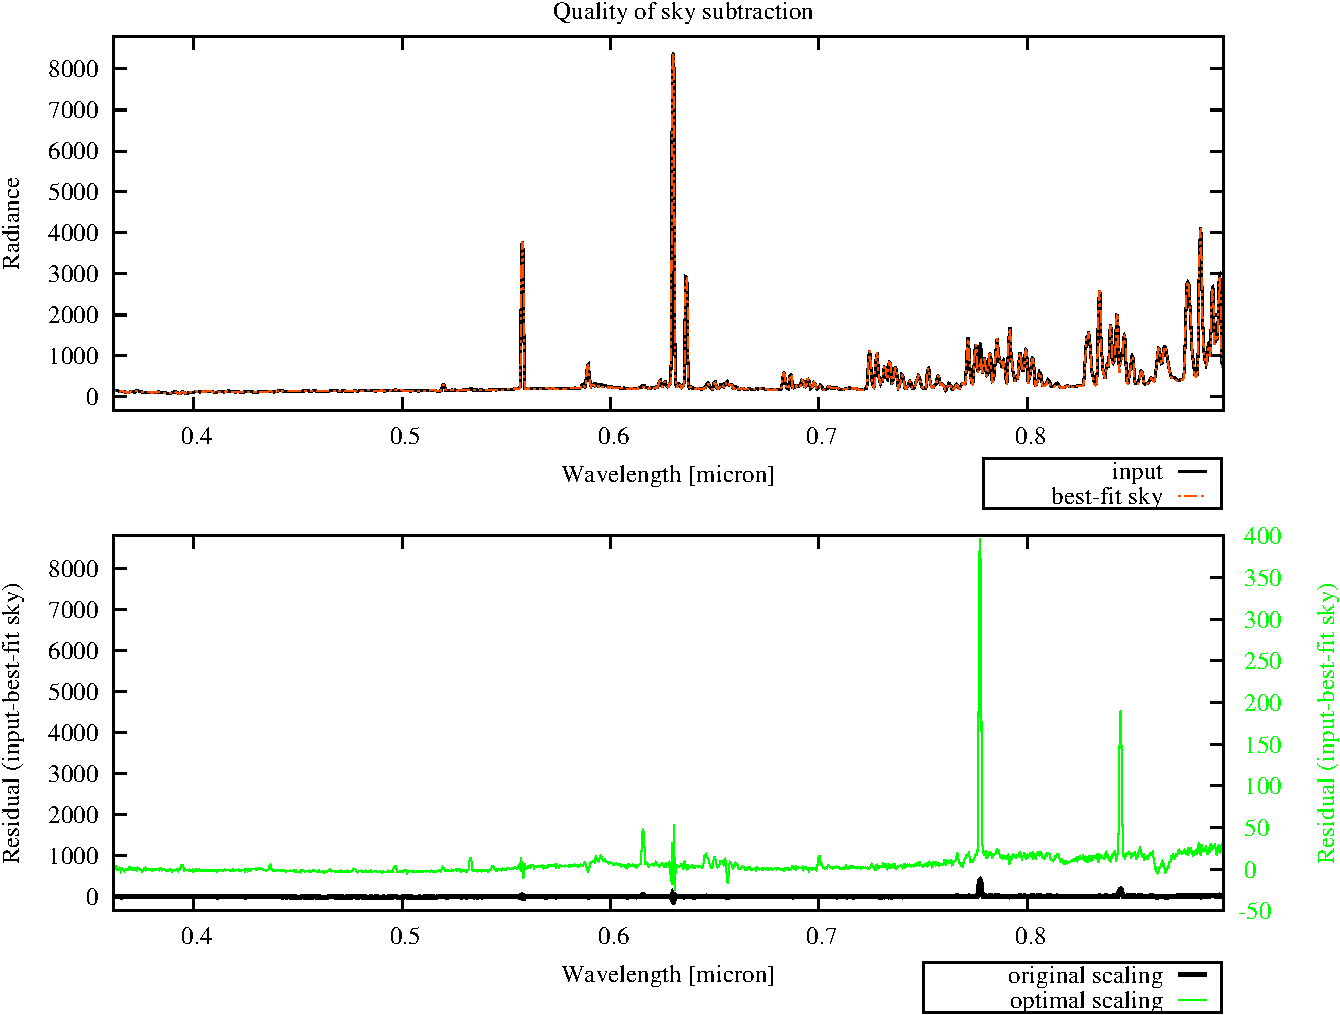
\includegraphics[width=0.7\textwidth,clip=true]{figures/TEST-FORS-1_fit.pdf}
\caption[]{Comparison of fors\_0918 (black) and best-fit fors\_0919 (red). The
upper panel shows the input and the best-fit spectra, the lower panel the
residual in two different scalings (black~=~original scaling, green~=~optimal
scaling).}
\label{fig:fors_1}
\end{figure}

\begin{figure}
\centering
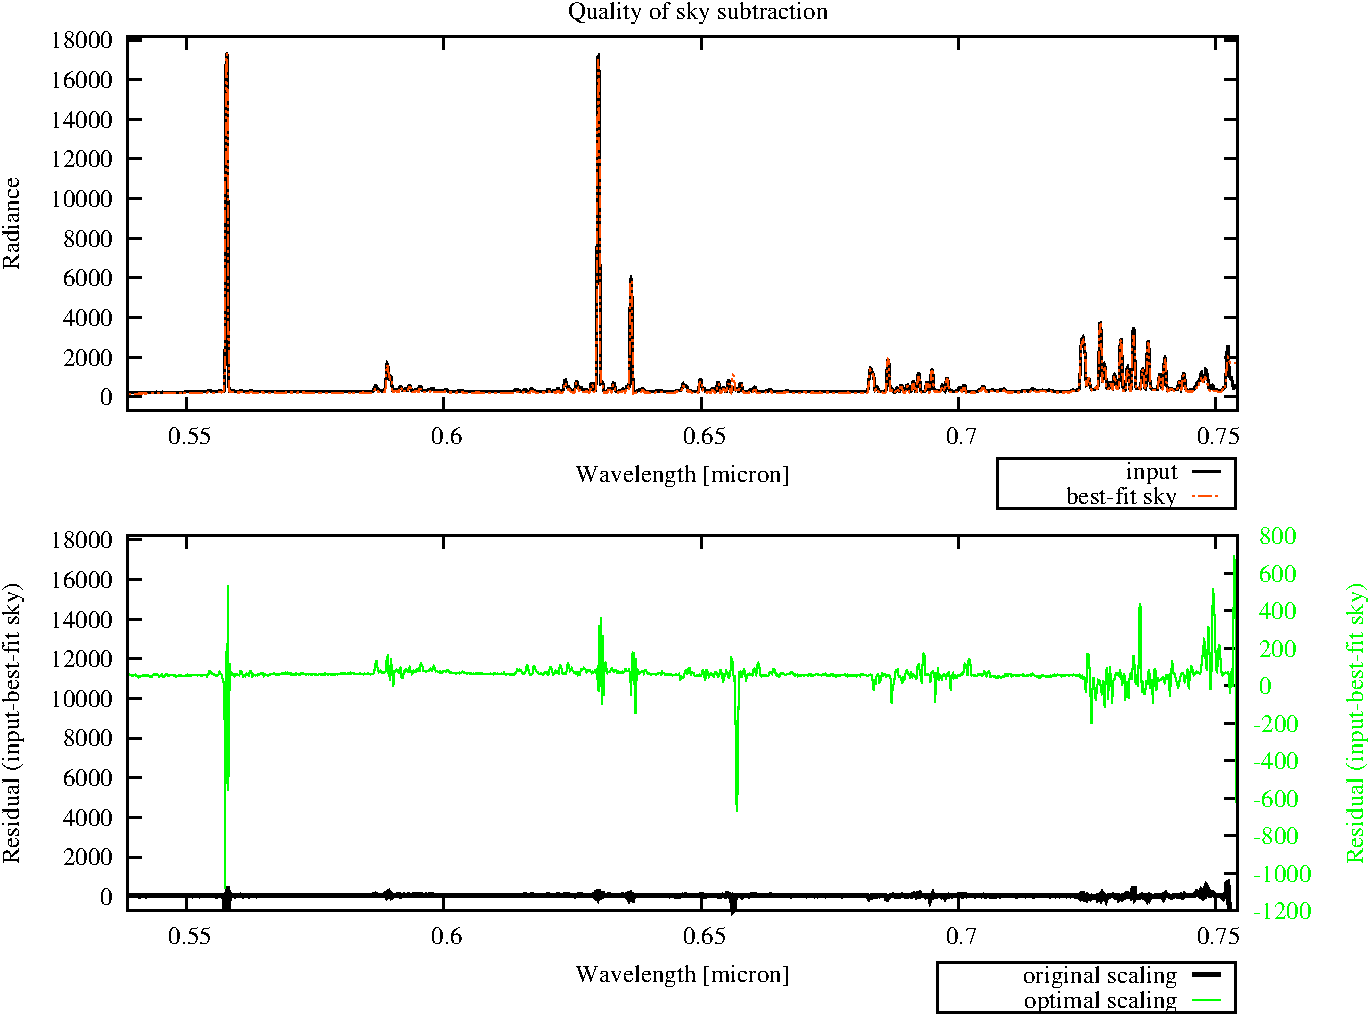
\includegraphics[width=0.7\textwidth,clip=true]{figures/TEST-FORS-4_fit.pdf}
\caption[]{Comparison of fors\_0114 (black) and best-fit fors\_1154 (red). The
upper panel shows the input and the best-fit spectra, the lower panel the
residual in two different scalings (black~=~original scaling, green~=~optimal
scaling).}
\label{fig:fors_4}
\end{figure}

\begin{figure}
\centering
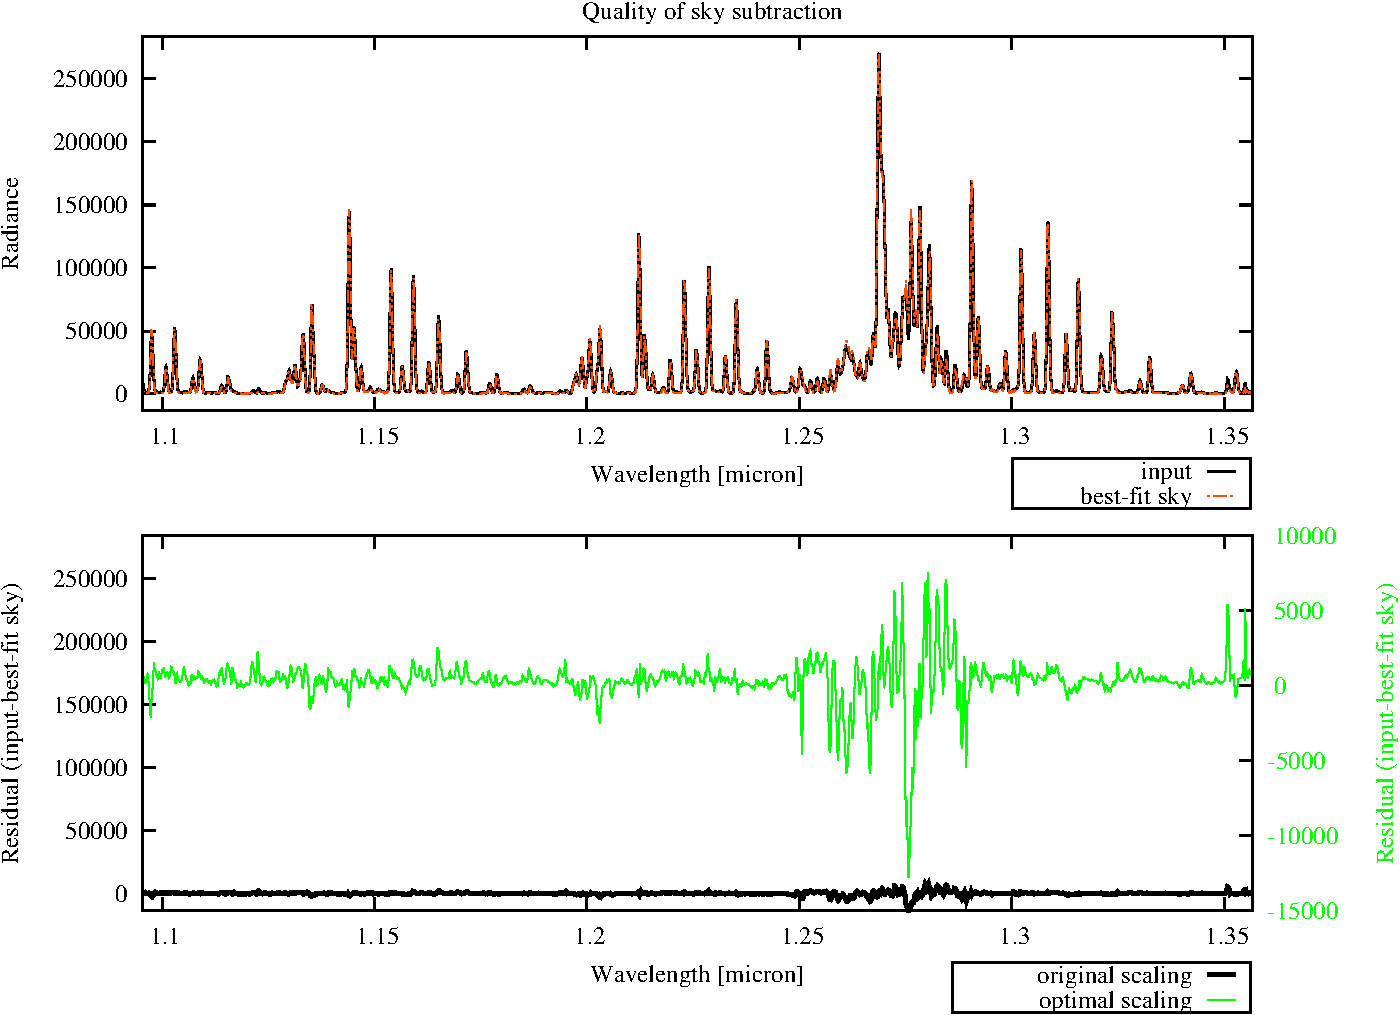
\includegraphics[width=0.7\textwidth,clip=true]{figures/TEST-SINFO-J_fit.pdf}
\caption[]{Comparison of sinfo\_6 (black) and best-fit sinfo\_7 (red). The
upper panel shows the input and the best-fit spectra, the lower panel the
residual in two different scalings (black~=~original scaling, green~=~optimal
scaling).}
\label{fig:sinfo_J}
\end{figure}

\begin{figure}
\centering
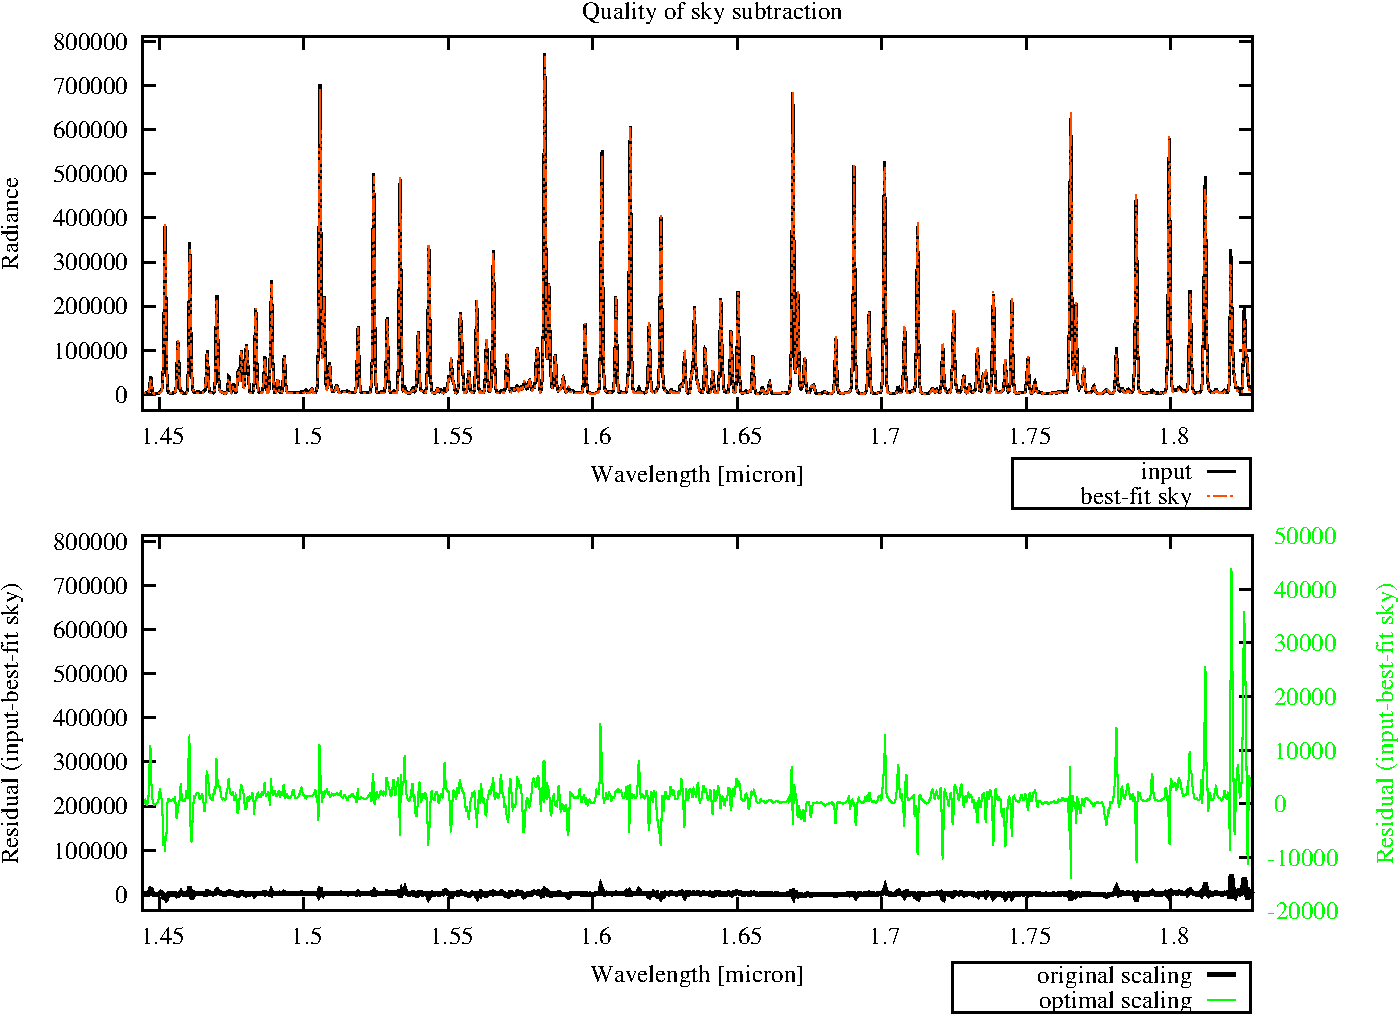
\includegraphics[width=0.7\textwidth,clip=true]{figures/TEST-SINFO-H_fit.pdf}
\caption[]{Comparison of sinfo\_1 (black) and best-fit sinfo\_2 (red). The
upper panel shows the input and the best-fit spectra, the lower panel the
residual in two different scalings (black~=~original scaling, green~=~optimal
scaling).}
\label{fig:sinfo_H}
\end{figure}

\begin{figure}
\centering
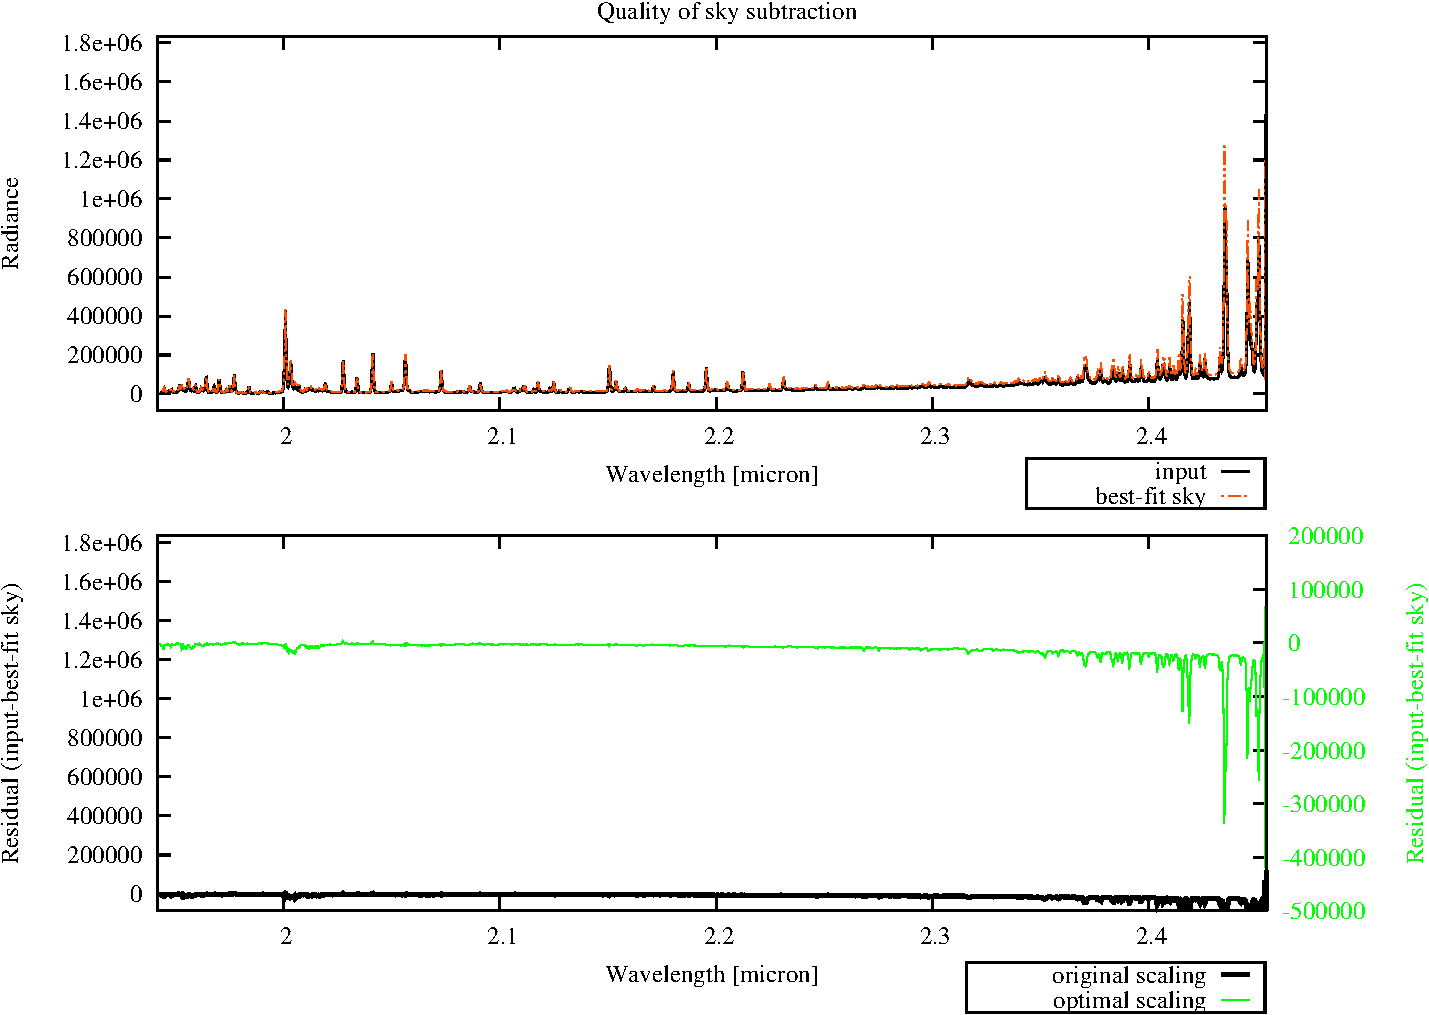
\includegraphics[width=0.7\textwidth,clip=true]{figures/TEST-SINFO-K_fit.pdf}
\caption[]{Comparison of sinfo\_4 (black) and best-fit sinfo\_5 (red). The
upper panel shows the input and the best-fit spectra, the lower panel the
residual in two different scalings (black~=~original scaling, green~=~optimal
scaling).}
\label{fig:sinfo_K}
\end{figure}

\begin{figure}
\centering
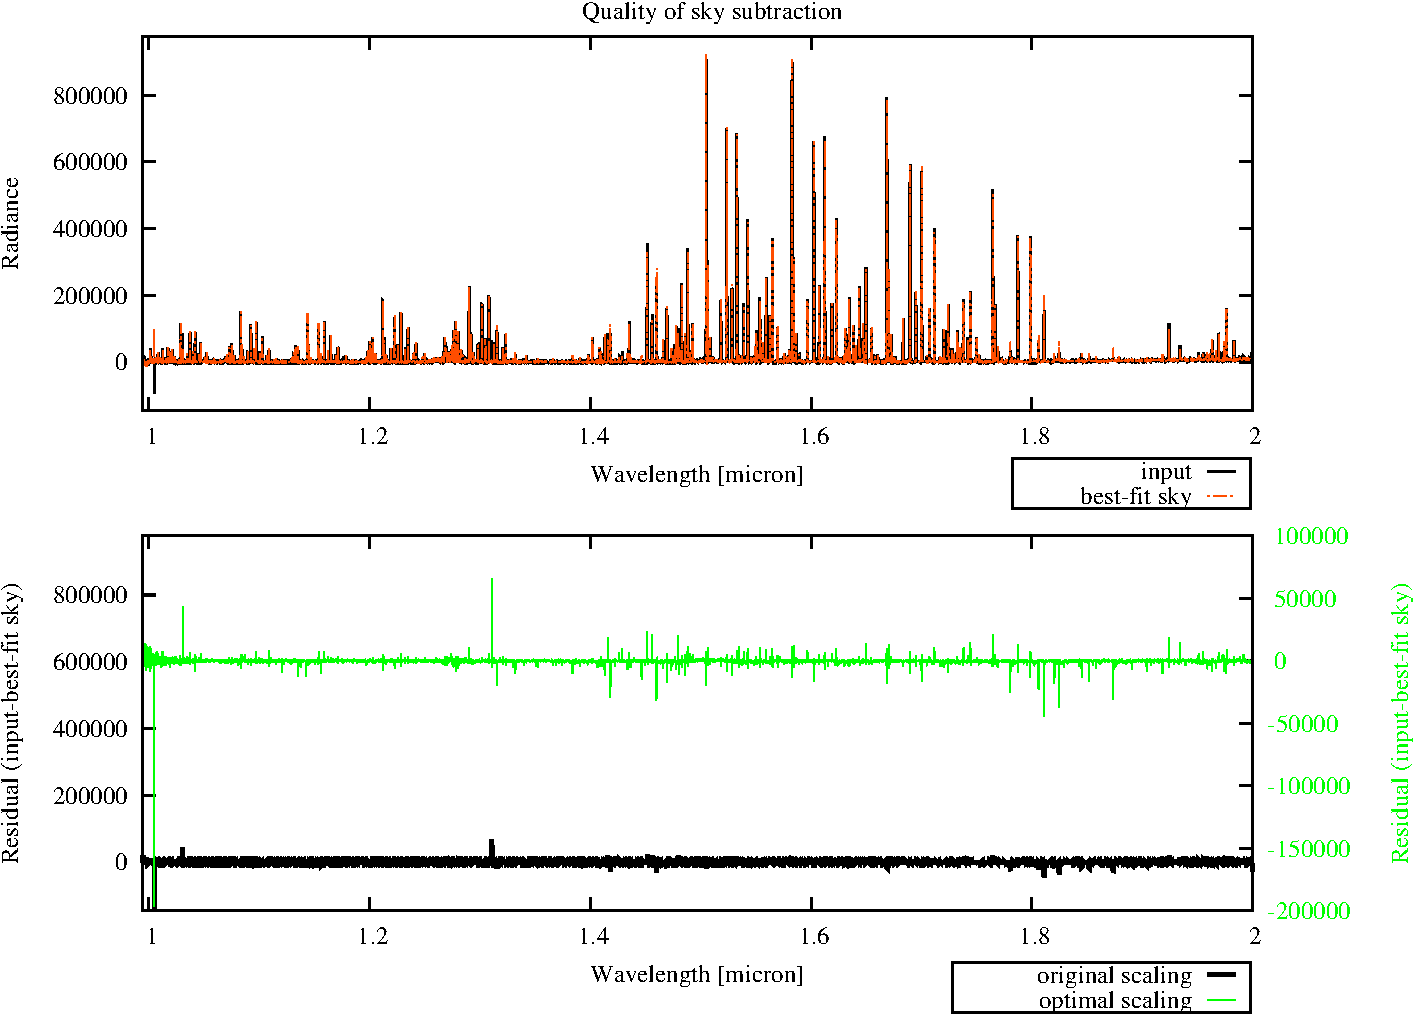
\includegraphics[width=0.7\textwidth,clip=true]{figures/TEST-XSHOO-1_fit.pdf}
\caption[]{Comparison of xshoo\_28 (black) and best-fit xshoo\_29 (red). The
upper panel shows the input and the best-fit spectra, the lower panel the
residual in two different scalings (black~=~original scaling, green~=~optimal
scaling).}
\label{fig:xshoo_1}
\end{figure}

\begin{figure}
\centering
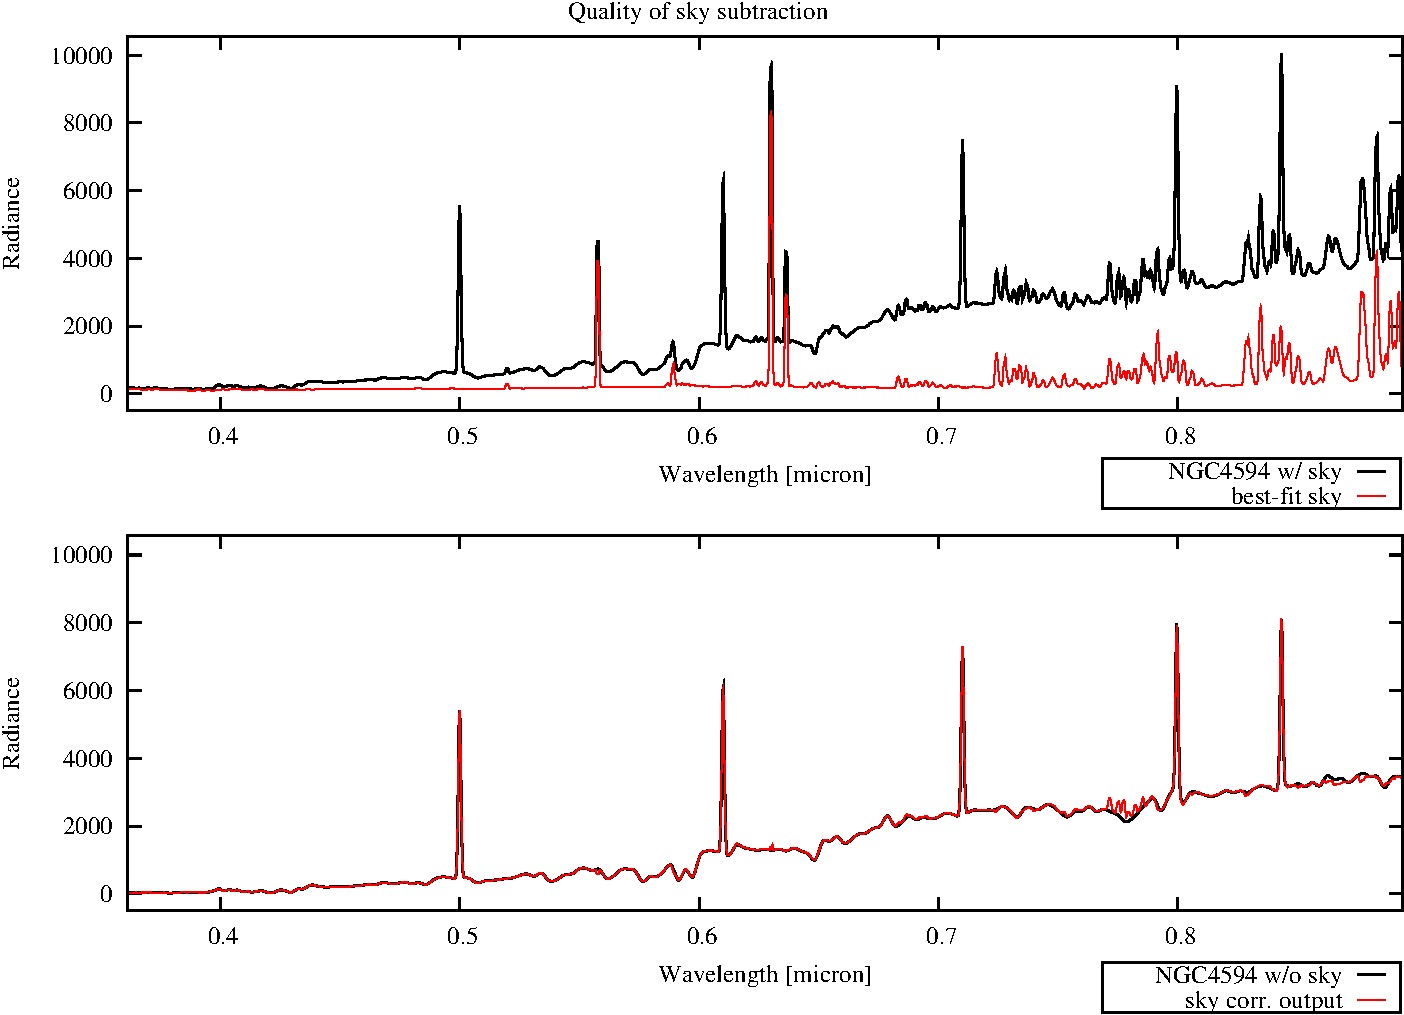
\includegraphics[width=0.7\textwidth,clip=true]
{figures/N4594-FORS_overplot_w_gal.pdf}
\caption[]{Comparison of arbitrarily scaled NGC\,4594 spectrum at $z = 0.5$ +
artificial emission lines of equal intensity at 0.5, 0.61, 0.71, 0.799553,
0.843248\,$\mu$m + fors\_0918 (black) and best-fit fors\_0919 (red). The lower
panel shows the sky subtraction residual (red) and the original, not
sky-affected NGC\,4594 spectrum (black).}
\label{fig:fors_1_n4594}
\end{figure}

\begin{figure}
\centering
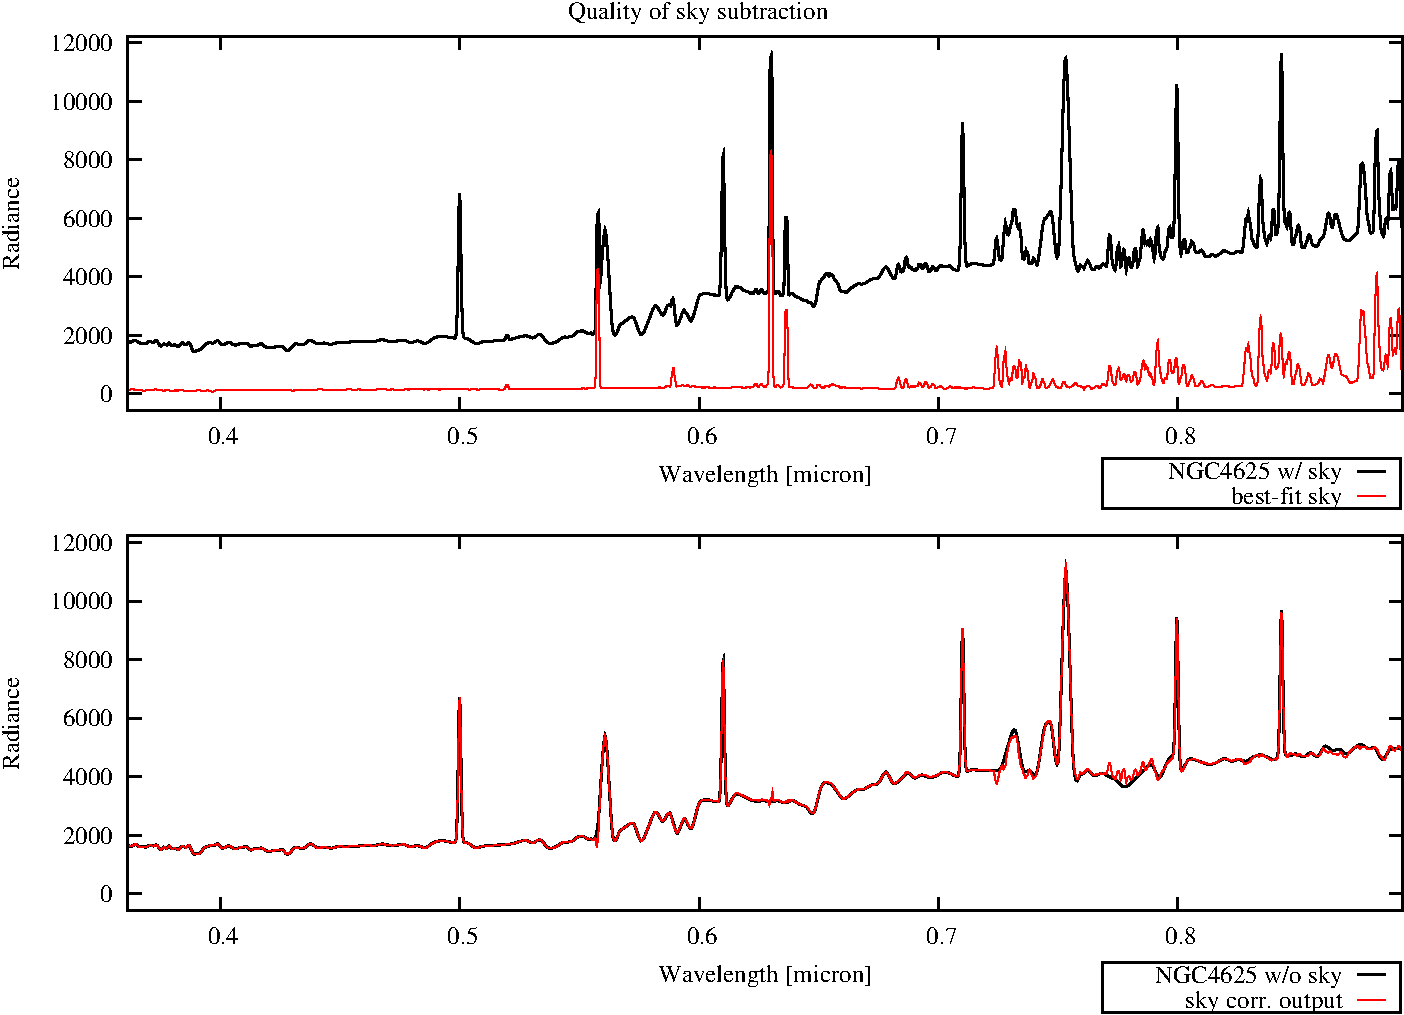
\includegraphics[width=0.7\textwidth,clip=true]
{figures/N4625-FORS_overplot_w_gal.pdf}
\caption[]{Comparison of arbitrarily scaled NGC\,4625 spectrum at $z = 0.5$ +
artificial emission lines of equal intensity at 0.5, 0.61, 0.71, 0.799553,
0.843248\,$\mu$m + fors\_0918 (black) and best-fit fors\_0919 (red). The lower
panel shows the sky subtraction residual (red) and the original, not
sky-affected NGC\,4625 spectrum (black).}
\label{fig:fors_1_n4625}
\end{figure}

\begin{figure}
\centering
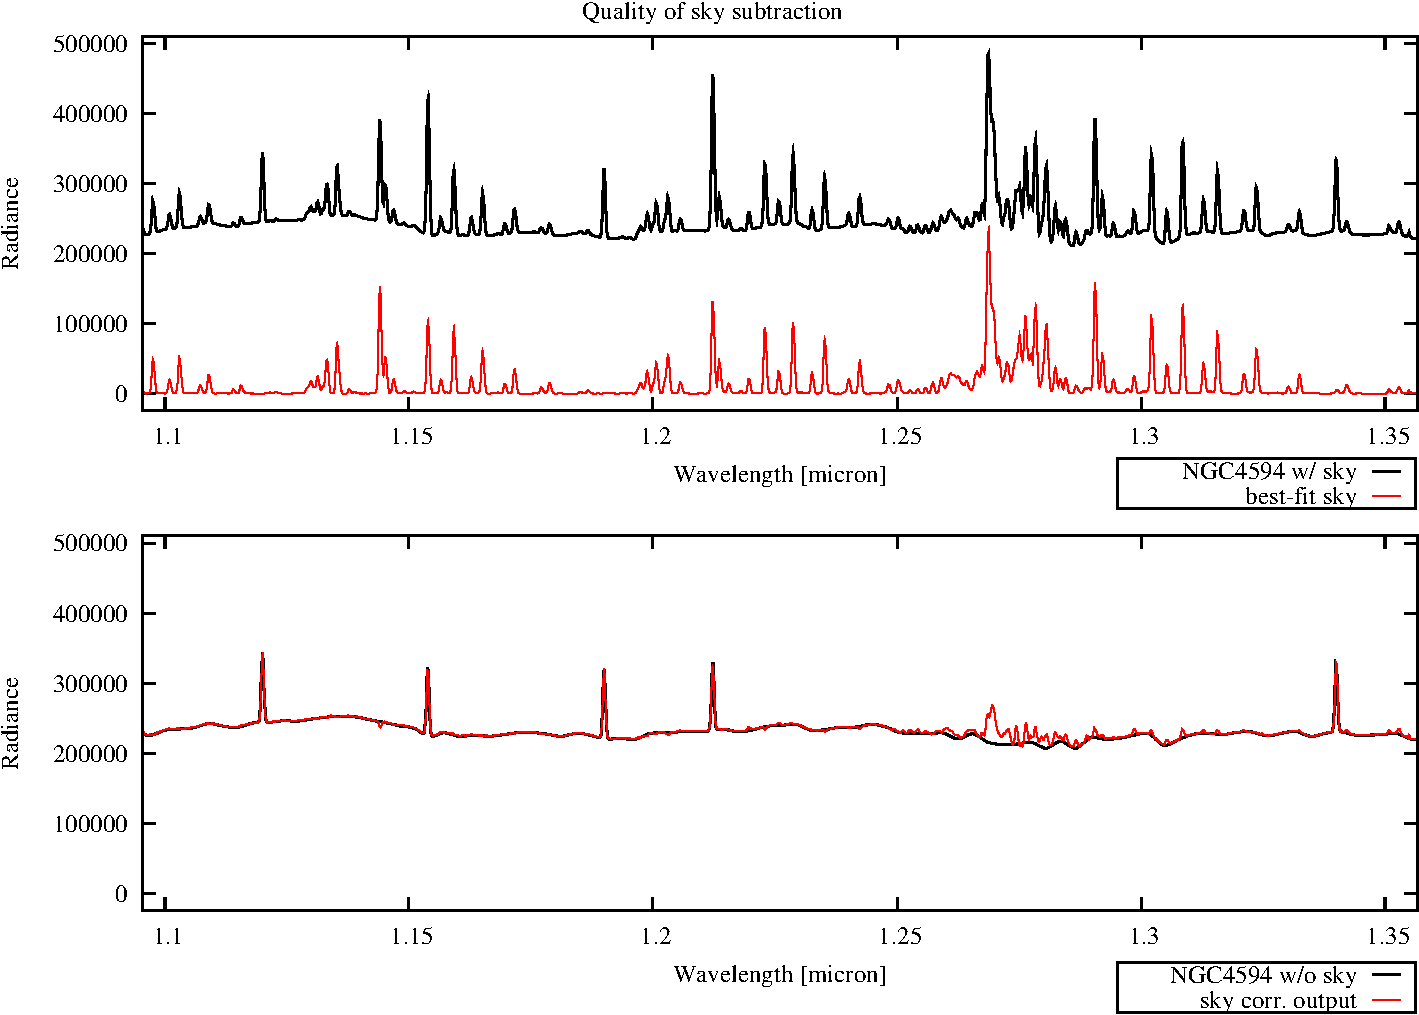
\includegraphics[width=0.7\textwidth,clip=true]
{figures/N4594-SINFO-J_overplot_w_gal.pdf}
\caption[]{Comparison of arbitrarily scaled NGC\,4594 at $z = 0.5$ + artificial
emission lines of equal intensity at 1.12, 1.153871, 1.19, 1.212263, and
1.34\,$\mu$m + sinfo\_6 (black) and best-fit sinfo\_7 (red). The lower panel
shows the sky subtraction residual (red) and the original, not sky-affected
NGC\,4594 spectrum (black).}
\label{fig:sinfo_J_n4594}
\end{figure}

\begin{figure}
\centering
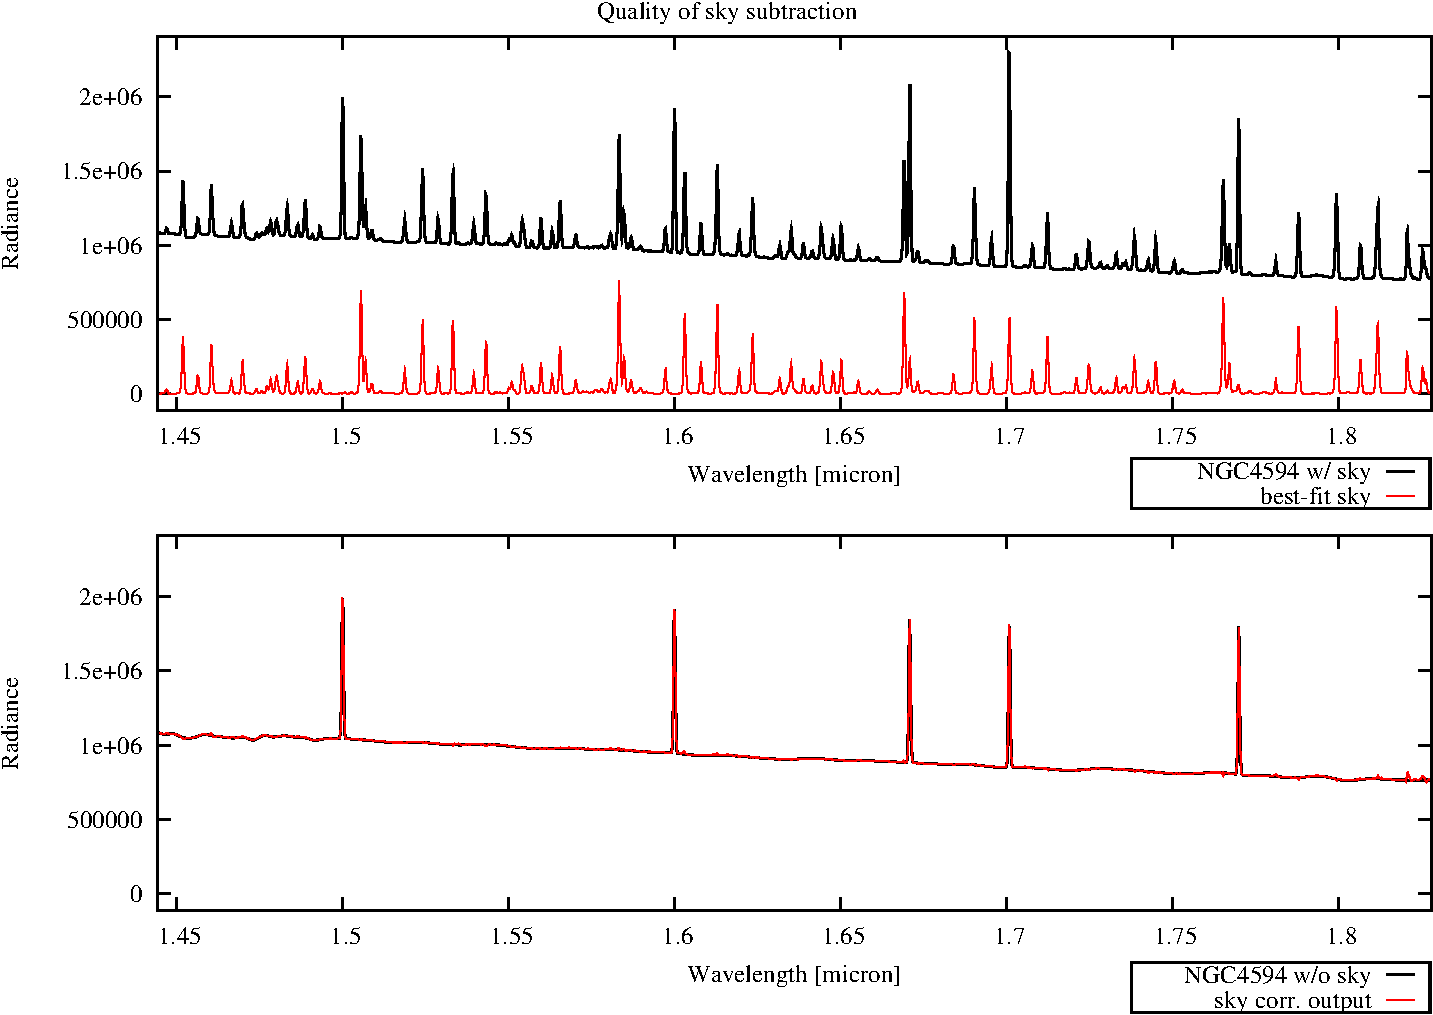
\includegraphics[width=0.7\textwidth,clip=true]
{figures/N4594-SINFO-H_overplot_w_gal.pdf}
\caption[]{Comparison of arbitrarily scaled NGC\,4594 at $z = 0.5$ + artificial
emission lines of equal intensity at 1.50, 1.60, 1.670881, 1.700843, and
1.77\,$\mu$m + sinfo\_1 (black) and best-fit sinfo\_2 (red). The lower panel
shows the sky subtraction residual (red) and the original, not sky-affected
NGC\,4594 spectrum (black).}
\label{fig:sinfo_H_n4594}
\end{figure}

\begin{figure}
\centering
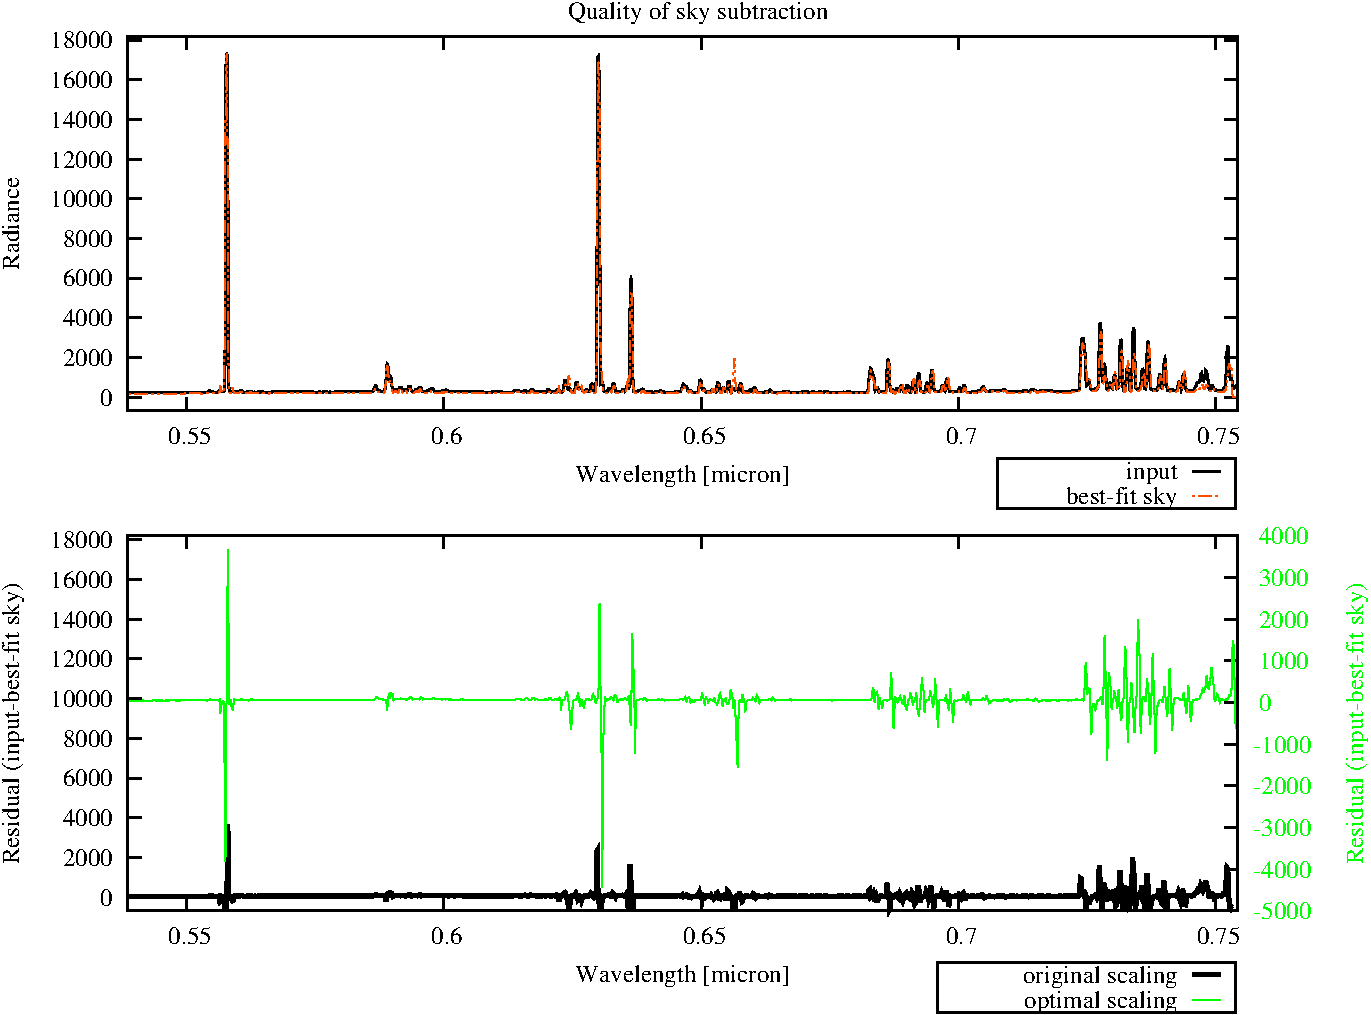
\includegraphics[width=0.7\textwidth,clip=true]{figures/TEST-FORS-4-NC_fit.pdf}
\caption[]{Comparison of fors\_0114 (black) and best-fit fors\_1154 (red) for
no correction of the wavelength grid by the fit of a Chebyshev polynomial. The
upper panel shows the input and the best-fit spectra, the lower panel the
residual in two different scalings (black~=~original scaling, green~=~optimal
scaling).}
\label{fig:fors_4_nc}
\end{figure}

The performance of SKYCORR is discussed in the following.
Section~\ref{sec:testsetup} describes the test set-up. The results are
discussed in Section~\ref{sec:results}. Finally, SKYCORR is compared to the
SINFONI pipeline procedure based on the Davies method
(Section~\ref{sec:compdavies}). Some test data are available in the code
directory {\tt <INST\_DIR>/examples/} (see
Section~\ref{sec:calling_examples}). This folder also contains a set of
X-Shooter spectra, which is extensively discussed in the project's science
report \cite{SM03SR}.

%-------------------------------------------------------------------------------
\subsection{Test set-up}\label{sec:testsetup}
%-------------------------------------------------------------------------------
SKYCORR was applied to sky spectra taken from the sky model verification data
set (see \cite{SM01} User Manual). Spectra from the FORS\,1, SINFONI, and
X-Shooter instruments were used (see Tables~\ref{tab:sample} and
\ref{tab:results_sky}). Davies' \cite{DAV07} method was developed for SINFONI
IR spectra. The present SINFONI data set comprises two $J$-band, two $H$-band,
and three $K$-band spectra. With these data a single test per band was
performed, using one spectrum as input science spectrum and one as reference
sky spectrum. The available SINFONI spectra are challenging for the sky
subtraction procedure, since the spectra of each band show exceptionally
pronounced differences (see \cite{SM01} User Manual). In addition, the $J$-band
spectra were taken about half a year apart. In order to have more realistic
input spectra, we also facilitate four pairs of X-Shooter NIR arm spectra
obtained with $0.9''$ and $1.5''$ slits, respectively. The two combinations for
each instrumental set-up differ in the time difference of both exposures. Short
time periods are in the order of one hour or one night, while long time spreads
are in the order of one month. For long time differences, the available sample
of X-Shooter spectra in not suitable. Finally, we also tested four pairs of
FORS\,1 sky spectra taken with the 300\,V and the 600\,R grism, respectively
(see Patat \cite{PAT08}). Thus, we can also test our code in the optical regime
and for low resolution. The resolution of the FORS spectra is about 500 and
1200, respectively, compared to values between 2000 and 5300 for the IR
spectra. For each grism, the exposure dates and times of the target spectra
were selected to differ from those of the fixed reference sky spectrum by the
order of one hour and several years, respectively. The very long periods
possible for the comprehensive FORS data set allow us to compare airglow
spectra taken during phases of significantly different solar activity.

Since the task of the sky correction procedure is the subtraction of sky
emission from an object spectrum showing a continuum and possible emission
lines, a test that corrects one sky spectrum to fit another one is
insufficient. Therefore, the sky spectra defined as science input were
manipulated by adding an object spectrum (see Table~\ref{tab:results_obj}). For
this, best-fit spectral energy distributions (SEDs) of the nearby galaxies
NGC\,4594 and NGC\,4625 obtained by means of the galaxy SED-fitting code CIGALE
(see Noll et al. \cite{NOL09}) were used. The spectra of the two NGC galaxies
are very different. While NGC\,4594 shows an early-type spectrum without
significant emission lines, NGC\,4625 is a late-type galaxy with strong
emission lines. In order to move more lines and continuum features into a
wavelength range where airglow is strong, the two galaxy SEDs were shifted
to a redshift of $z = 0.5$. The flux of the object spectra was scaled
arbitrarily. The SEDs were scaled such that they exhibit a similar strength as
the airglow emission lines. Since the CIGALE model spectra were optimised to fit
photometry (see Noll et al. \cite{NOL09}), the resolution of the emission lines
in the NGC\,4625 spectrum is significantly lower than the resolution of our
observed test sky spectra. In order to test the code for object emission lines
having the same resolution as the sky lines (and to compensate for the lack of
galaxy emission lines in the near-IR), we added 15 artificial lines of constant
intensity to the NGC\,4594 and NGC\,4625 spectra. Lines were set at 0.5, 0.61,
0.71, 0.799553, 0.843248, 1.12, 1.153871, 1.19, 1.212263, 1.34, 1.50, 1.60,
1.670881, 1.700843, and 1.77\,$\mu$m. Since the positions of 6 lines coincide
with strong OH lines, the conservation of object line strength by the sky
correction procedure can be investigated. The final object spectra were added
to a representative subsample of the 11 target sky spectra defined as science
input (see Table~\ref{tab:results_sky}), which resulted in $2 \times 5$
different test set-ups with object spectrum (see Table~\ref{tab:results_obj}).

For a better comparison of the results and to check the quality of the sky
subtraction with standard parameters, we used identical input parameter files
differing in the input and output file names and the selection of air or
vacuum wavelengths only. The values of the fixed parameters can be found in the
listing of the example parameter file shown in Section~\ref{sec:paramfile}.
The Tables~\ref{tab:results_sky} and \ref{tab:results_obj} exhibit some results
for each test set-up. First, the number of fit parameters is shown. The number
of relevant A and B line group parameters (see Section~\ref{sec:airglow})
depends on the wavelength range covered by the spectra. Moreover, the rejection
of unreliable lines can cause that line groups are not fittable and have to be
scaled by mean factors (see Section~\ref{sec:linefit}). The number of
coefficents of the Chebyshev polynomial for the wavelength grid correction (see
Section~\ref{sec:wavegrid}) is variable, since an automatic search for the best
degree is set by default (see Section~\ref{sec:paramfile}). Then, the ranges of
fitted line group flux correction factors are shown for the A and B groups.
Note that the correction factors for lines groups of OH and O$_2$ can differ
considerably. On the other hand, the range of scaling factors of groups of the
same system (\eg\ OH) can be significantly less spread than implied by the
interval given in the table. As indicator for the quality of the sky correction
procedure, Table~\ref{tab:results_sky} shows the weighted RMS derived from
the difference between best-fit reference sky and input science line peak flux
(no continuum) relative to the mean line peak flux in the science spectrum.
Values in the order of a few per cent can be considered as good. Moreover, the
mean ratio $\langle \frac{\Delta f_\mathrm{peak}}{f_\mathrm{peak}} \rangle$ of sky
correction residual and line flux for a $\sigma$-clippped selection of fitted
line peaks in the science spectrum is exhibited. This second quality measure
can be compared to the relative RMS values. If it is distinctly lower, the
RMS appears to be dominated by a few very strong residuals, since
$\langle \frac{\Delta f_\mathrm{peak}}{f_\mathrm{peak}} \rangle$ is relatively
insensitive to residuals that are much stronger than the average. For a visual
inspection of the fit quality Figures~\ref{fig:fors_1} to
\ref{fig:sinfo_H_n4594} show several representative comparisons between
best-fit sky and input science spectra. Finally, the results tables present the
execution times of the sky line fit and the entire code for each set-up. For
comparing the execution times, it should be noted that the X-Shooter spectra
used have 16766 pixels, which is about an order of magnitude higher than the
2048, 1741, 1921, and 2041 pixels of the FORS, SINFONI $J$-band, SINFONI
$H$-band, and SINFONI $K$-band spectra, respectively. Moreover, a degree of the
optimal Chebyshev polynomial above the minimum degree of 3 of the iterative
polynomial searching algorithm is related to a relatively long execution time,
since for each additional degree the line fitting procedure has to be repeated
(see Section~\ref{sec:wavegrid}).

%-------------------------------------------------------------------------------
\subsection{Results}\label{sec:results}
%-------------------------------------------------------------------------------
In general, the results of the sky correction procedure are satisfying. If only
the results for sky spectra (without science object) as shown in
Table~\ref{tab:results_sky} and Figures~\ref{fig:fors_1} to \ref{fig:xshoo_1}
are compared, the best fits are obtained for the first and third FORS set-up
for which the tabulated RMS is below 1\%. For these set-ups the time
difference between both exposures is very short, \ie\ in the order of one hour
(see Table~\ref{tab:sample}). However, even for combinations of spectra taken
with several years in between the fits are good. The relatively low
S/N of the X-Shooter spectra prevent better RMS values than those given in
the table. Significant systematic residuals are rare. An example are the
insufficently corrected O\,I multiplets at 777 and 845\,nm of the first FORS
set-up (see Figure~\ref{fig:fors_1}). Usually these ionospheric lines are weak
and difficult to detect among the strong OH lines. However, in the case of the
target sky spectrum, a strong amplification of these lines occurred, which was
much stronger than for the other ionospheric lines that mainly determine the
correction of the A\,3 group (see Table~\ref{tab:Agroups}). Consequently, there
are certain situations which impede a good correction of atomic lines
originating in the thermosphere. However, the potentially affected wavelength
ranges are very narrow. Another wavelength range which is difficult to correct
is at about 1.27\,$\mu$m. Figure~\ref{fig:sinfo_J} indicates conspicuous
residuals there. The reason is the presence of a strong O$_2$ band (see
Figure~\ref{fig:o2a00band}) with many overlapping lines at the resolution of
SINFONI in the $J$-band. Hence, the continuum determination and the line group
flux correction is very difficult in this wavelength range. For the case of the
SINFONI example the correction was particularly challenging, since the
intensities of the O$_2$(a-X)(0-0) band in the two input spectra differ by an
extreme factor of about 7 (see Table~\ref{tab:results_sky}). In contrast, the
O$_2$ band correction worked much better for the X-Shooter spectra. The example
shown in Figure~\ref{fig:xshoo_1} only indicates minor residuals. Reasons for
the improved results are probably the lower correction factors ($< 4$) and
the higher resolution (see Table~\ref{tab:sample}). Finally,
Figure~\ref{fig:sinfo_K} exhibiting the results of the SINFONI $K$-band set-up
shows relatively strong residuals beyond 2.3\,$\mu$m. Sky lines in the
remaining spectrum are corrected very well. The emission lines at long
wavelengths (beyond 2.3\,$\mu$m) cannot be corrected by our sky subtraction
code, since these are caused by thermal emission in the lower atmosphere and
not airglow emission in the upper atmosphere. Consequently, the code does not
scale line fluxes in the thermal IR. Note that a high degree of the Chebyshev
polynomial for the wavelength grid correction could be a problem in this
regime because of the required strong extrapolation. The example in
Figure~\ref{fig:sinfo_K} does not seem to be affected by this issue. However,
it shows that the subtracion of the strong thermal continuum, which is mainly
caused by the telescope main mirror and cannot be fitted, can be a problem if
the mirror temperature changes between the science and sky exposures.

Adding an object to the input science frame --quite expectedly-- usually causes
a decrease in the fit quality (see Table~\ref{tab:results_obj}). Nevertheless,
in general, the resulting sky-subtracted spectra are good. Examples are shown
in Figures~\ref{fig:fors_1_n4594} to \ref{fig:sinfo_H_n4594}. Due to a strong
and complex continuum, it can happen that the line group correction factors
become less reliable if the continuum has to be interpolated over a relatively
wide wavelength range. This appears to be the reason for the relatively poor
correction of the OH(9-4) band in the object FORS spectra shown in
Figure~\ref{fig:fors_1_n4594} and \ref{fig:fors_1_n4625} and the
O$_2$(a-X)(0-0) band in the object SINFONI $J$-band spectra (see
Figure~\ref{fig:sinfo_J_n4594}). The X-Shooter spectra complemented by an
object spectrum are much better corrected in this wavelength regime as a
comparison of Tables~\ref{tab:results_obj} and \ref{tab:results_sky} implies.
Here, the relatively high resolution has probably helped to better constrain
the continuum. Figures~\ref{fig:fors_1_n4594} to \ref{fig:sinfo_H_n4594}
illustrate the efficiency of SKYCORR in conserving the flux of object emission
lines. The relatively broad lines of the galaxy spectra and the 5 narrow
artificial lines (with FWHM matching that of the spectral set-up) are well
conserved. Even lines directly positioned on top of airglow lines are regained
almost perfectly. A requirement for such a good fit is that the object lines
are masked by the $\sigma$-clipping approach described in
Section~\ref{sec:linefit}. At least for the tested spectra the algorithm works
very well.

The repeated fitting of airglow lines for different degrees of the Chebyshev
polynomial for the wavelength grid correction (see Section~\ref{sec:wavegrid})
imposes a penalty on the code execution times. Run times from 4 to 97\,s are
tabulated in Tables~\ref{tab:results_sky} and \ref{tab:results_obj}. Most of
this time is consumed by the iterative line fitting procedure. The code can be
accelerated considerably by setting the parameter {\sc cheby\_max} to -1 (see
Section~\ref{sec:paramfile}). In this case, no wavelength correction is
performed. This may be an option for spectra with very good wavelength
calibration. However, if the wavelengths grids of two spectra indicate
significant deviations, it is much better to perform the default fitting
procedure. This is demonstrated by Figure~\ref{fig:fors_4_nc} which shows the
results of the fourth FORS set-up (see Table~\ref{tab:results_sky}) without any
wavelength correction. Compared to Figure~\ref{fig:fors_4} which exhibits the
sky-subtracted spectrum for the standard run, the residuals in
Figure~\ref{fig:fors_4_nc} are extremely strong. The spectrum fors\_0114, which
was taken about four and a half years before the reference spectrum fors\_1154
does not appear to be well calibrated. For example, the central wavelength of
the O\,I line at 557.7\,nm differs by about half a pixel. In this case a good
wavelength grid correction is mandatory. This result justifies the choice
of {\sc cheby\_max}~=~7 and {\sc cheby\_min}~=~3 for the standard run, which
aims at providing acceptable sky-corrected spectra for all kinds of input data.

%-------------------------------------------------------------------------------
\subsection{Comparison to Davies' code}\label{sec:compdavies}
%-------------------------------------------------------------------------------
For a concluding evaluation of the performance of SKYCORR, it is required to
compare the present results to those of Davies' code, which is part of the
SINFONI data reduction pipeline (see Section~\ref{sec:davies}).

%-------------------------------------------------------------------------------
\subsubsection{Results for the test set-up}\label{sec:restest}
%-------------------------------------------------------------------------------
\begin{table}
\caption[]{Comparison of SKYCORR and Davies' code}
\label{tab:davies}
\centering
\vspace{5pt}
\begin{tabular}{l c c c c}
\hline\hline
\noalign{\smallskip}
Sample$^\mathrm{a}$ &
$\frac{RMS_\mathrm{SKYCORR}}{\langle f_\mathrm{peak} \rangle}$$^\mathrm{b}$ [\%] &
$\frac{RMS_\mathrm{Davies}}{\langle f_\mathrm{peak} \rangle}$$^\mathrm{b}$ [\%] &
$\frac{RMS_\mathrm{SKYCORR}}{RMS_\mathrm{Davies}}$ [\%] &
$\frac{\langle|\Delta|\rangle_\mathrm{SKYCORR}}
{\langle|\Delta|\rangle_\mathrm{Davies}}$$^\mathrm{c}$ [\%] \\
\noalign{\smallskip}
\hline
\noalign{\smallskip}
Pure sky & $3.9 \pm 2.9$ & $9.7 \pm 8.0$ & $47.4 \pm 21.0$ & $41.0 \pm 15.4$ \\
Object + sky & $4.8 \pm 5.3$ & $7.6 \pm 7.8$ & $60.4 \pm \ \, 9.0$ &
$46.1 \pm \ \, 6.2$ \\
All & $4.4 \pm 4.2$ & $8.6 \pm 7.7$ & $54.3 \pm 16.6$ & $43.7 \pm 11.3$ \\
\noalign{\smallskip}
\hline
\end{tabular}
\footnotesize
\begin{list}{}{}
\item[$^\mathrm{a}$] FORS spectra are not considered, since Davies' code cannot
handle wavelengths below 1\,$\mu$m.
\item[$^\mathrm{b}$] RMS (and its scatter) from difference between residual
flux of sky correction by SKYCORR or Davies' code and pure object spectrum
(zero line for pure sky spectra) relative to mean flux of science spectrum line
peaks (flag~$\ge 2$; see Section~\ref{sec:linesearch}). For the RMS, all
pixels are considered except for wavelengths beyond 2.3\,$\mu$m, where emission
from the lower atmosphere dominates the spectra.
\item[$^\mathrm{c}$] Ratio of results of SKYCORR and Davies' code for mean
absolute difference between residual flux of sky correction and pure object
spectrum. Only wavelengths up to 2.3\,$\mu$m are considered.
\end{list}
\end{table}

\begin{figure}
\centering
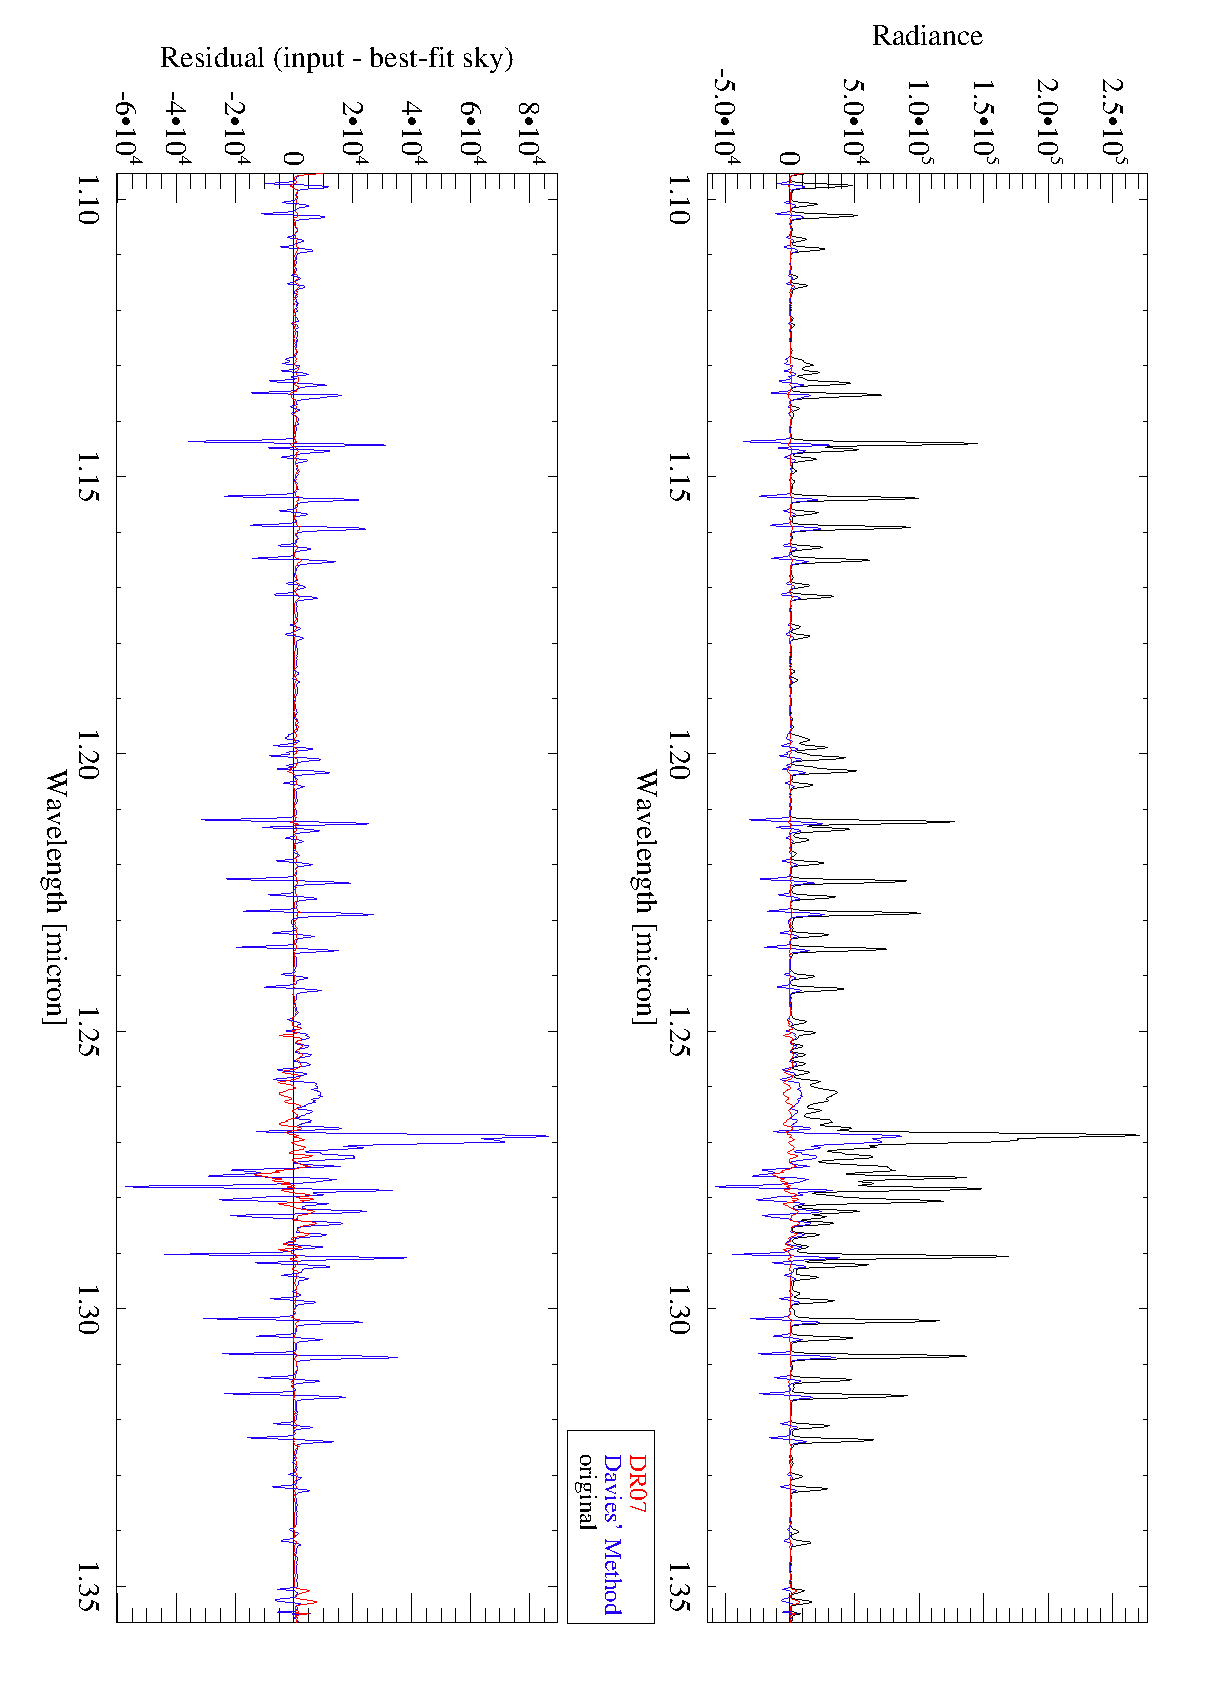
\includegraphics[width=8.8cm,clip=true,angle=90]
{figures/TEST-SINFO-J_comp.eps}
\caption[]{Comparison of SKYCORR (red) and Davies' code results (blue) for the
SINFONI $J$-band set-up without object spectrum (cf. Figure~\ref{fig:sinfo_J}).
Apart from the residuals of the sky correction procedure the upper panel also
shows the input science spectrum (black).}
\label{fig:sinfo_J_comp}
\end{figure}

\begin{figure}
\centering
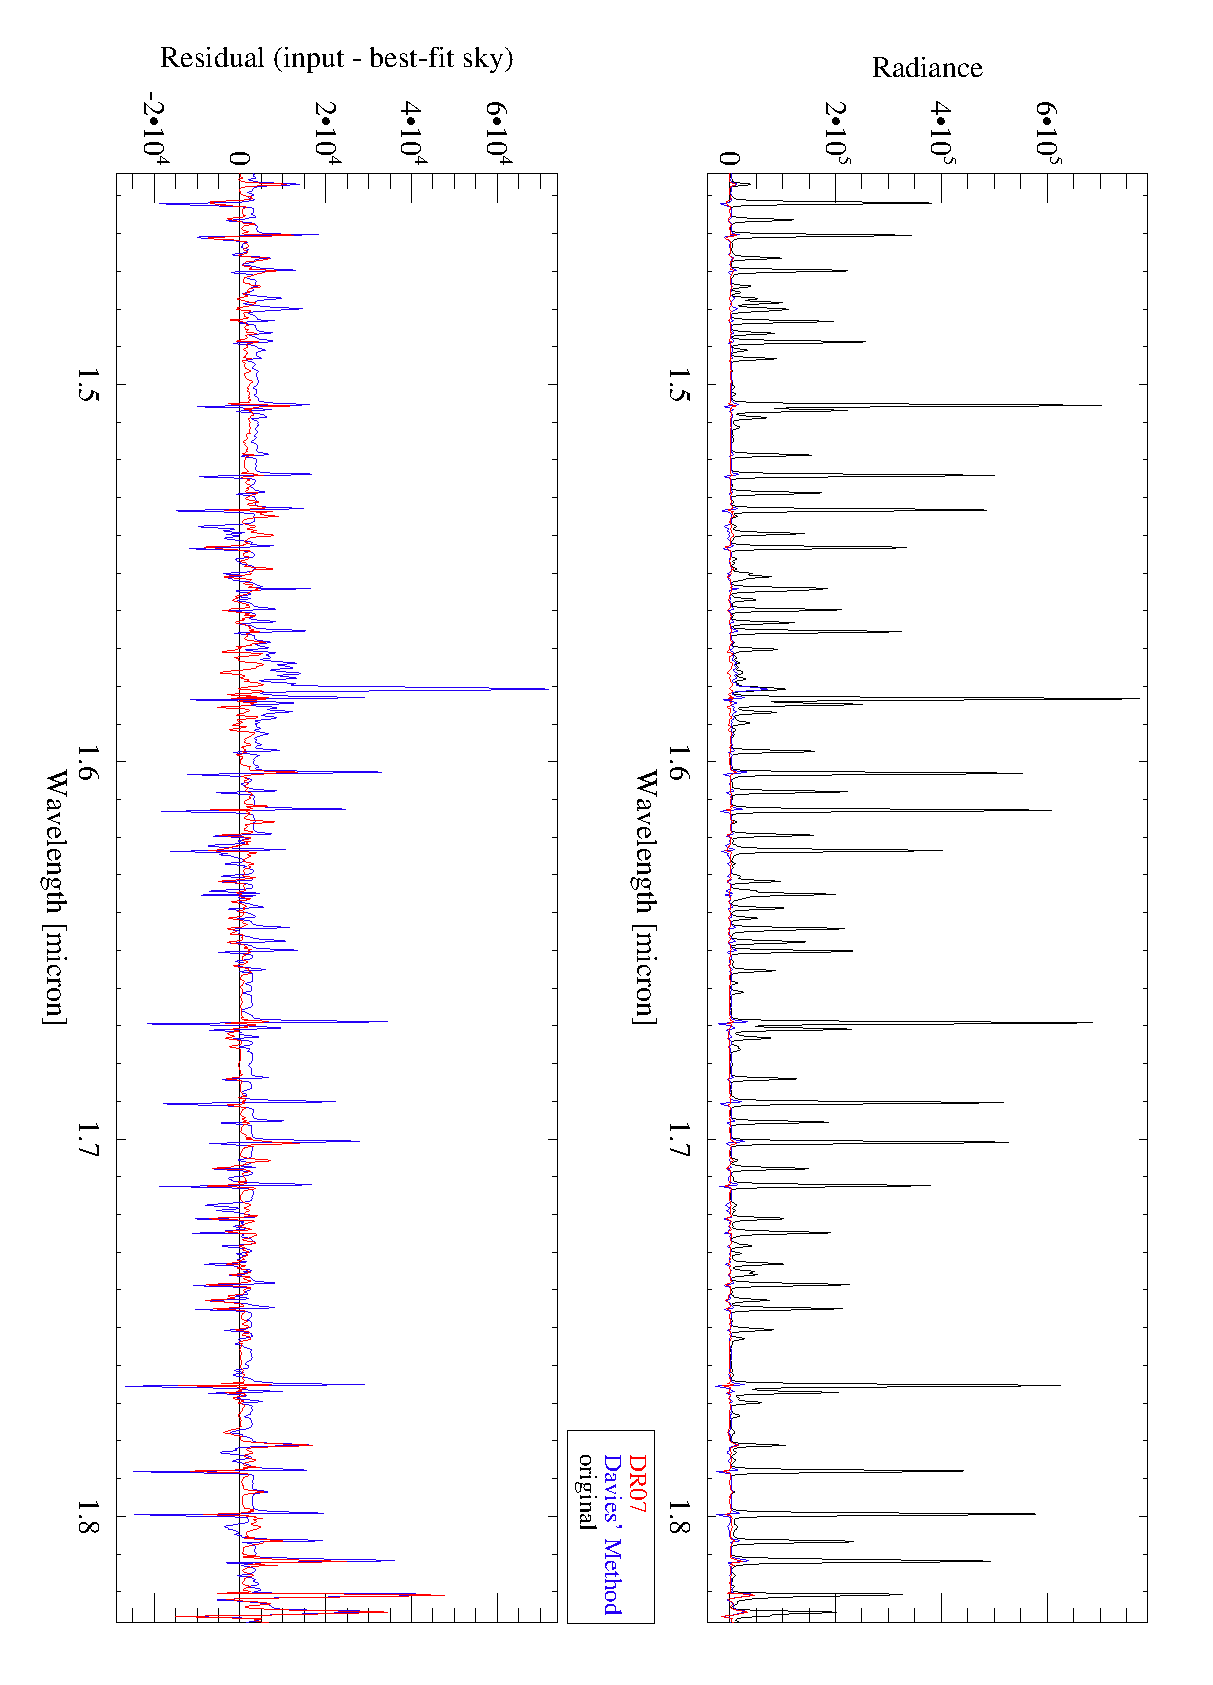
\includegraphics[width=8.8cm,clip=true,angle=90]
{figures/TEST-SINFO-H_comp.eps}
\caption[]{Comparison of SKYCORR (red) and Davies' code results (blue) for the
SINFONI $H$-band set-up without object spectrum (cf. Figure~\ref{fig:sinfo_H}).
Apart from the residuals of the sky correction procedure the upper panel also
shows the input science spectrum (black).}
\label{fig:sinfo_H_comp}
\end{figure}

\begin{figure}
\centering
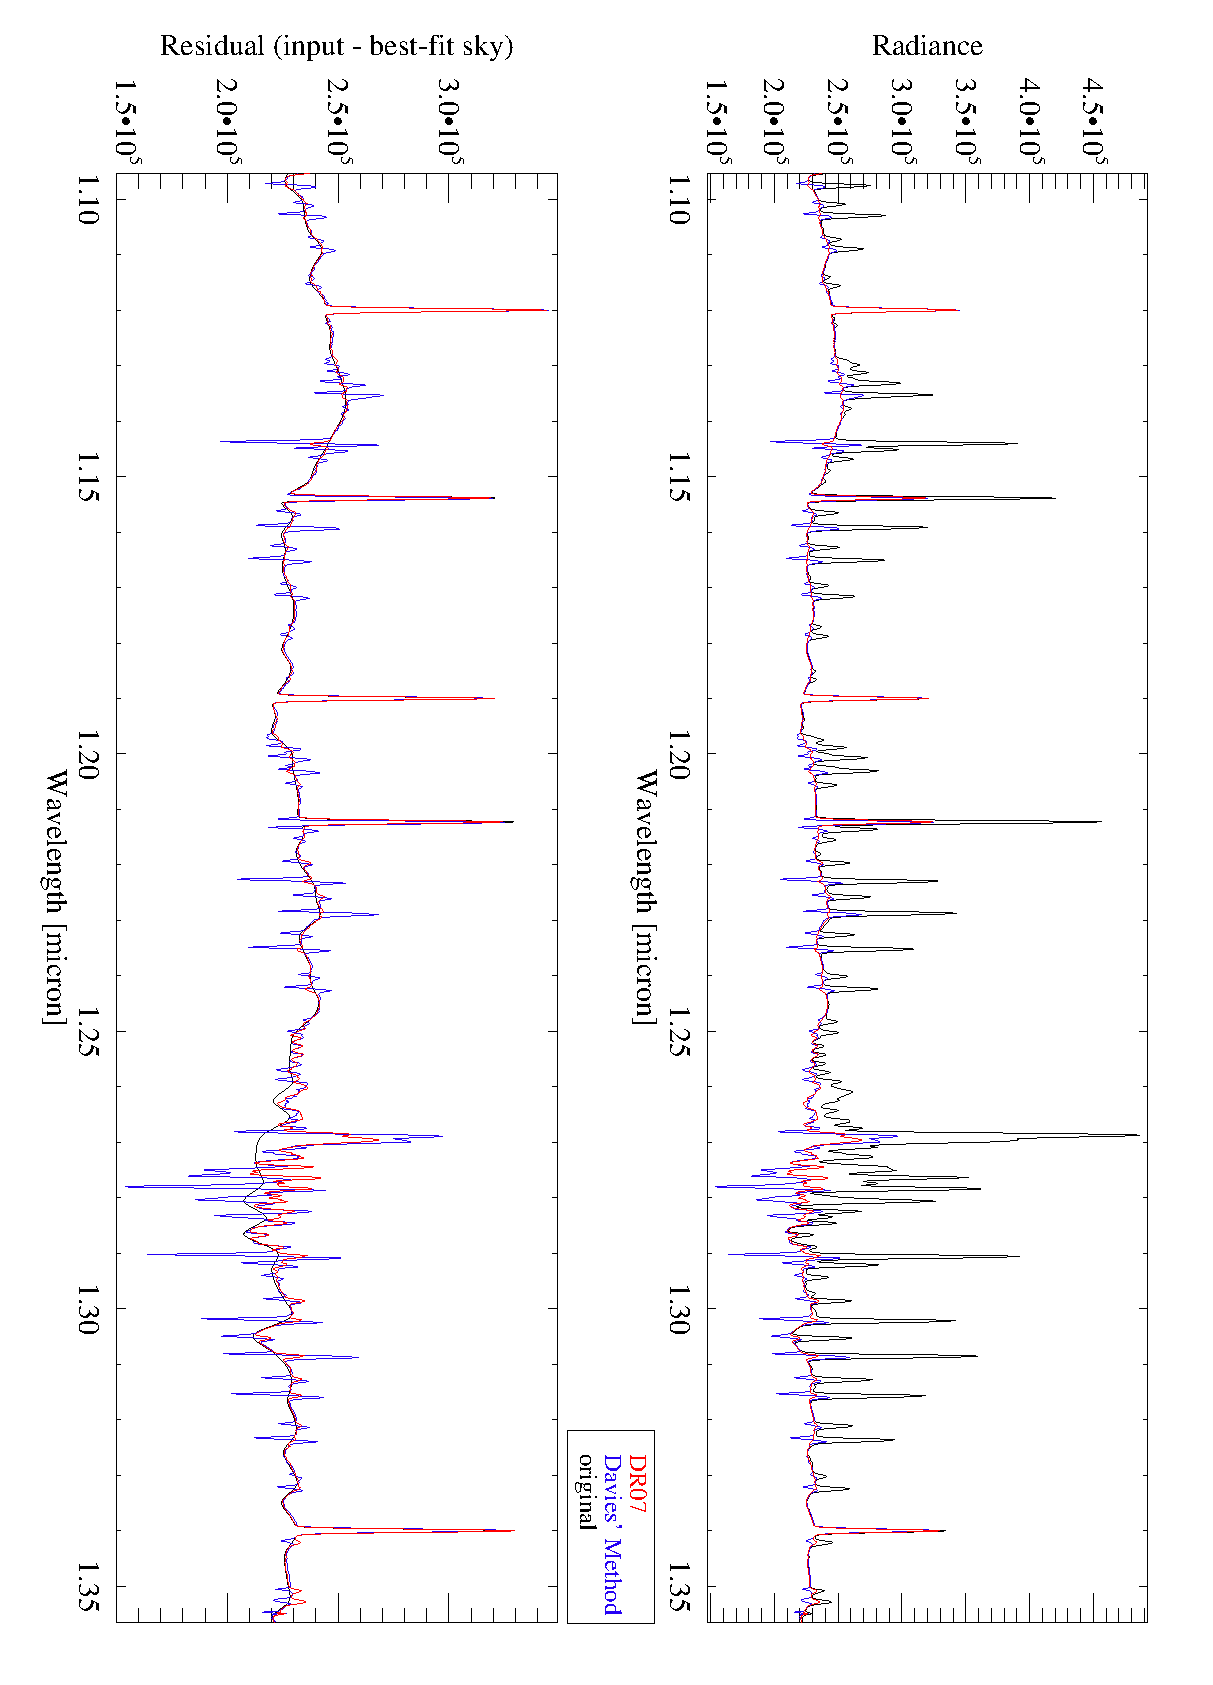
\includegraphics[width=8.8cm,clip=true,angle=90]
{figures/N4594-SINFO-J_comp.eps}
\caption[]{Comparison of SKYCORR (red) and Davies' code results (blue) for the
SINFONI $J$-band set-up with object spectrum (cf.
Figure~\ref{fig:sinfo_J_n4594}). Apart from the residuals of the sky correction
procedure the upper panel also shows the input science spectrum (black).}
\label{fig:sinfo_J_n4594_comp}
\end{figure}

A slightly adapted version of Davies' code was run on our test data set
described in Section~\ref{sec:testsetup}. The FORS set-ups have not been
tested, since Davies' code is not able to correct airglow lines at wavelengths
below 1\,$\mu$m. Consequently, the resulting test data set consists of 7 pure
sky and 8 object + sky set-ups. The results of the runs of both codes are
summarised in Table~\ref{tab:davies}. The listing exhibits the relative RMS
mean values and their scatter for the subsample of pure sky spectra, the
subsample of object spectra, and the total sample of 15 set-ups. In contrast to
Tables~\ref{tab:results_sky} and \ref{tab:results_obj}, the RMS was computed
for all pixels of the spectrum. Moreover, the RMS calculation is related to the
difference between the residual of the sky correction and the input object
spectrum which is a zero line for pure sky spectra. The RMS values of both
codes are provided relative to the mean line peak flux in the input science
spectrum. In order to simplify the comparison of the results of both codes, the
ratio of both RMS values is shown as well. Finally, a corresponding ratio for
the mean absolute difference between sky correction residual and pure object
spectrum is indicated. In comparison to the RMS ratio, the latter quantity is
less sensitive to very strong residuals that affect a few pixels only. For this
reason, a high RMS compared to the mean absolute difference suggests that
strong residuals affect a relatively narrow range of the spectrum only.
Examples for the differences in the results of both codes are presented in
Figures~\ref{fig:sinfo_J_comp} to \ref{fig:sinfo_J_n4594_comp}.

Table~\ref{tab:davies} indicates that SKYCORR has an improved performance in
comparison to Davies' code. In the tested set-ups, the RMS of SKYCORR is
lower. On average the RMS ratio is about 54\%. For pure sky spectra, the
results tend to be better than for science spectra incorporating an object
(47\% versus 60\%). This discrepancy is not observed for the mean absolute
difference, where the results for the two subsamples differ from the mean of
44\% only slightly. The differences in the results for both quantities can be
explained --as already mentioned above-- by the dominance of the contribution
to the RMS by a few residual pixels. Such a situation is shown in
Figure~\ref{fig:sinfo_J_n4594_comp}, which indicates relatively strong
residuals for the O$_2$ band at 1.27\,$\mu$m. Apart from the O$_2$ band, where
both codes are comparable, the SKYCORR performance is superior (by a factor of
2 on average). However, this particular band cannot be corrected very well,
since the density of strong lines is very high requiring interpolation of the
continuum over a relatively wide wavelength range. As already discussed in
context of Figure~\ref{fig:sinfo_J}, the interpolation, the complex object
continuum, and the extreme difference in the properties of the two sky spectra,
prevent a good sky correction in this wavelength range.

%-------------------------------------------------------------------------------
\subsubsection{Results for SINFONI pipeline data}\label{sec:ressinfo}
%-------------------------------------------------------------------------------
\begin{figure}
\centering
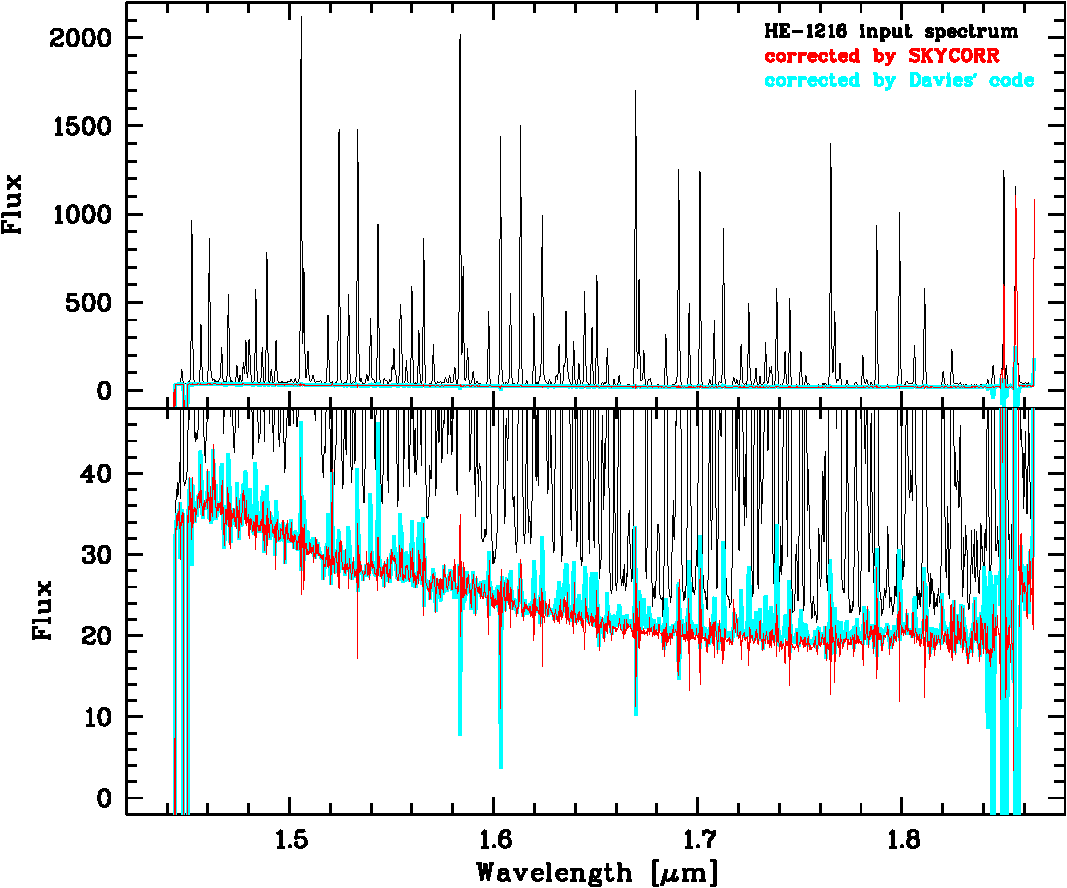
\includegraphics[width=0.7\textwidth,clip=true]
{figures/scr_comp_sinfo_H_ex1.pdf}
\caption[]{Comparison of SKYCORR (red) and Davies' code results (cyan) for a
SINFONI $H$-band pipeline product. While the upper panel shows the full input
spectrum of HE\,1216, the lower panel focuses on the sky subtraction results.}
\label{fig:sinfo_H_ex1}
\end{figure}

\begin{figure}
\centering
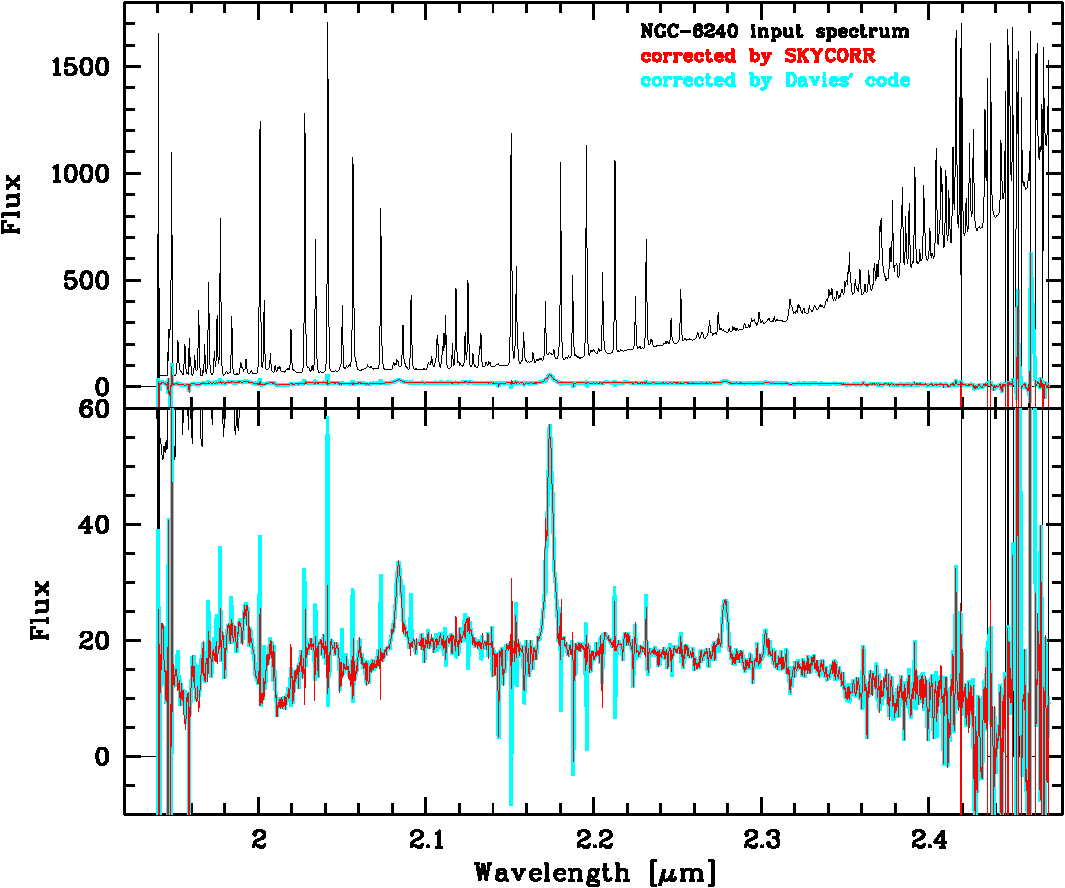
\includegraphics[width=0.7\textwidth,clip=true]
{figures/scr_comp_sinfo_K_ex1.pdf}
\caption[]{Comparison of SKYCORR (red) and Davies' code results (cyan) for a
SINFONI $K$-band pipeline product. While the upper panel shows the full input
spectrum of NGC\,6240, the lower panel focuses on the sky subtraction results.}
\label{fig:sinfo_K_ex1}
\end{figure}

\begin{figure}
\centering
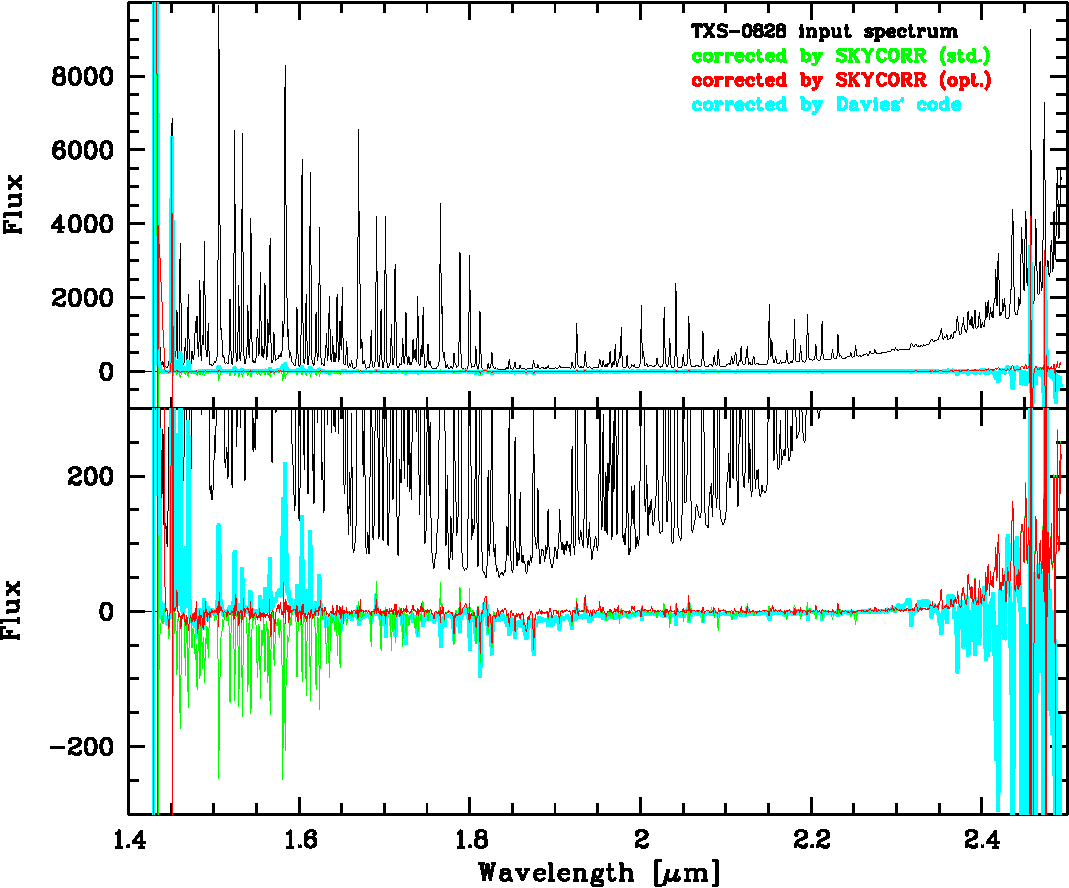
\includegraphics[width=0.7\textwidth,clip=true]
{figures/scr_comp_sinfo_HK_ex1.pdf}
\caption[]{Comparison of SKYCORR (green/red) and Davies' code results (cyan)
for a SINFONI $HK$-band pipeline product. SKYCORR was run for the default
parameter set (green; see Section~\ref{sec:paramfile}) and an optimised
set-up (red), which only differs from the standard by
{\sc min\_line\_dist}~=~12.5. While the upper panel shows the full input
spectrum of TXS\,0828, the lower panel focuses on the sky subtraction results.}
\label{fig:sinfo_HK_ex1}
\end{figure}

For the code evaluation by means of sky model verification data and simulated
object spectra (see Section~\ref{sec:restest}), Davies' code was modified to
handle data that was not processed with this routine before. In order to get a
better idea how SKYCORR would perform if it was used in the SINFONI pipeline
(Modigliani et al.~\cite{MOD07}) instead of the Davies method, one could also
modify the SINFONI pipeline products to allow an application of SKYCORR. For
this purpose, suitable object and reference sky 1D data derived from SINFONI
data cubes for spectroscopic observations in different bands were provided by
A. Modigliani from ESO.

In Figures~\ref{fig:sinfo_H_ex1} to \ref{fig:sinfo_HK_ex1}, we illustrate the
performance of SKYCORR for this realistic data set comprising observations in
the $H$, $K$, and $HK$-band modes. The results are superb for $H$ and $K$ with
relative residuals of about three orders of magnitude weaker than the original
airglow lines. Moreover, the comparison to the Davies code indicates a
significantly better sky subtraction by SKYCORR, which is in agreement with the
results of Section~\ref{sec:restest}. The results of the $HK$ mode are worse
for both codes with residuals up to several per cent. For the default parameter
set-up, the quality of the SKYCORR sky-subtracted spectrum is relatively
similar to the one produced by Davies' code. However, the wavelength position
and shape of the residuals are very different. As demonstrated by
Figure~\ref{fig:sinfo_HK_ex1}, an optimisation of the SKYCORR input parameter
set can distinctly improve the results. To achieve the convincing sky
subtraction, only the {\sc min\_line\_dist} parameter (see
Section~\ref{sec:params}) was set from 2.5 to 12.5. Likewise, another good
result was obtained by changing {\sc fluxlim} from -1 to 0.08. These changes
affect the line finder (Section~\ref{sec:linesearch}) and the separation of
lines and continuum (Section~\ref{sec:contsub}). This makes sense, since the
resolution of the SINFONI $HK$-band mode is relatively low (about 1500;
cf.~Table~\ref{tab:sample}), which causes enhanced line blending. Hence,
the line detection and continuum separation becomes difficult if pseudo
continua consisting of line blends cover large parts of the investigated
spectrum. In particular, the $H$ band around the O$_2$ band at 1.58\,\mum{}
characterised by a high line density (see Figure~\ref{fig:o2a01band}) appears
to be affected by this issue.

Summarising the evaluation section, we can conclude that the SKYCORR sky
correction code produces convincing results for various kinds of data even if
the time period between the object and reference sky exposures is very long. In
general, the results are better than those produced by Davies' code. In most
cases, good sky subtraction can be achieved with a minimum of interaction. If
this is not sufficient, the user can try to fine-tune the sky subtraction by
varying the procedure's input parameters (see Section~\ref{sec:params}). Also,
this will influence the code run time.

\cleardoublepage
\section*{Acronyms}
\begin{acronym}
\acro{ASCII}{American Standard Code for Information Interchange}
\acro{CPL}{Common Pipeline Library}
\acro{ESO}{European Southern Observatory}
\acro{FITS}{Flexible Image Transport System}
\acro{FORS}{FOcal Reducer and low dispersion Spectrograph}
\acro{FWHM}{full width at half maximum}
\acro{GUI}{Graphical User Interface}
\acro{HITRAN}{High-resolution transmission molecular absorption database}
\acro{IDL}{Interactive Data Language}
\acro{IR}{infrared}
\acro{ISAAC}{Infrared Spectrometer and Array Camera}
\acro{LBLRTM}{Line-by-line Radiative Transfer Model}
\acro{RMS}{root mean square}
\acro{SED}{spectral energy distribution}
\acro{sfu}{solar flux units}
\acro{SINFONI}{Spectrograph for INtegral Field Observations in the Near
Infrared}
\acro{S/N}{signal-to-noise ratio}
\acro{UVES}{Ultraviolet and Visual Echelle Spectrograph}
\acro{VIMOS}{Visible Multi-Object Spectrograph}
\acro{VLT}{Very Large Telescope}
\end{acronym}


\begin{thebibliography}{99}

\section*{{\hspace{-\leftmargin}}References}

\bibitem[2005]{CLO05}
Clough, S.A, Shephard, M.W., Mlawer. E.J., et al. 2005, J. Quant. Spectrosc.
Radiat. Transfer, 91, 233

\bibitem[2006]{COS06}
Cosby, P.C., Sharpee, B.D., Slanger, T.G., Huestis, D.L., \& Hanuschik, R.W.
2006, J. Geophys. Res., 111, A12307

\bibitem[2007]{DAV07}
Davies, R.I. 2007, MNRAS, 375, 1099

\bibitem[1998]{GOL98}
Goldman, A., Schoenfeld, W.G., Goorvitch, D., et al. 1998, J. Quant. Spectrosc.
Radiat. Transfer, 59, 453

\bibitem[2003]{HAN03}
Hanuschik, R.W. 2003, A\&A, 407, 1157

\bibitem[2008]{KHO08}
Khomich, V.Y, Semenov, A.I., \& Shefov, N.N. 2008, Airglow as an Indicator of
Upper Atmospheric Structure and Dynamics, Springer, Berlin

\bibitem[1974]{MIE74}
Mies, F.H. 1974, J. Molec. Spectrosc., 53, 150

\bibitem[2007]{MOD07}
Modigliani, A., Hummel, W., Abuter, R., et al. 2007, The SINFONI pipeline,
arXiv:astro-ph/0701297

\bibitem[2010]{MOD10}
Modigliani. A., Goldoni, P., Royer, F., et al. 2010, Proc. SPIE, 7737, 773728

\bibitem[1980]{MOR80}
Mor\'e, J.J., Garbow, B.S., \& Hillstrom, K.E. 1980, User Guide for MINPACK-1,
Argonne National Laboratory Report ANL-80-74, Argonne, Ill.

\bibitem[2009]{NOL09}
Noll, S., Burgarella, D., Giovannoli, E., et al. 2009, A\&A, 507, 1793

\bibitem[2012]{NOL12}
Noll, S., Kausch, W., Barden, M., et al. 2012, A\&A, 543, A92

\bibitem[2008]{PAT08}
Patat, F. 2008, A\&A, 481, 575

\bibitem[2009]{ROT09}
Rothman, L.S., Gordon, I.E., Barbe, A., et al. 2009, J. Quant. Spectrosc.
Radiat. Transfer, 110, 533

\bibitem[2000]{ROU00}
Rousselot, P., Lidman, C., Cuby, J.-G., Moreels, G., \& Monnet, G. 2000, A\&A,
354, 1134

\bibitem[SM-01]{SM01}
SM-01 User Manual, VLT-MAN-ESO-19550-5770\\[0.5cm]

\bibitem[MOLECFIT]{MOLECFIT}
MOLECFIT User Manual, VLT-MAN-ESO-19550-5772\\[0.5cm]

\bibitem[SM-SoW]{SM-SoW}
Statement of Work for SM projects, VLT-SOW-ESO-19550-5223\\[0.5cm]

\bibitem[SM-03-SR]{SM03SR}
SM-03 Science Report, VLT-TRE-ESO-19550-5775 \\[0.5cm]

\bibitem[Reflex-UM]{reflex}
Reflex User Manual, VLT-MAN-ESO-19000-5037 \\[0.5cm]

\subsection*{{\hspace{-\leftmargin}}Links}

\bibitem[1]{CMPFIT}
\texttt{http://www.physics.wisc.edu/~craigm/idl/cmpfit.html}

\bibitem[2]{AER}
\texttt{http://www.aer.com/}

\bibitem[3]{HITRAN}
\texttt{http://www.cfa.harvard.edu/HITRAN/}

\bibitem[4]{SINC}
\texttt{http://www.astro.washington.edu/docs/idl/htmlhelp/slibrary30.html}

\bibitem[5]{huber}
AMC Technical Briefs - ISSN 1757-5958, No.6, Royal Society of Chemistry,
2001, \texttt{http://www.rsc.org/images/brief6\_tcm18-25948.pdf}

\bibitem[6]{LBLRTM}
\texttt{http://rtweb.aer.com/lblrtm\_frame.html}

\bibitem[7]{CPL}
\texttt{http://www.eso.org/sci/software/cpl}

\end{thebibliography}

\centerline{--- End of document ---}            % only if that's an even page

\end{document}
